\documentclass[11pt]{article}

\usepackage{times}
\usepackage{subfig}
\usepackage{amsfonts}
\usepackage{epsfig}
\usepackage{wrapfig}
\usepackage{graphicx}
\DeclareGraphicsExtensions{.pdf,.png,.jpg}
\usepackage{verbatim}
\usepackage{amsmath}
\usepackage{amssymb}
\usepackage{pifont}
\usepackage{array}
\usepackage{paralist}
\usepackage{multirow}
\usepackage{subcaption} % add this in the preamble
\usepackage{subfigure}
\usepackage[table,xcdraw]{xcolor}

\usepackage[pagebackref=true,breaklinks=true,colorlinks,bookmarks=false]{hyperref} 

\usepackage{jacobsn}

\setcounter{tocdepth}{2}

\newcommand{\ditem}[1]{\item {\sc #1}\hspace{.1in}}
\newcommand{\todo}[1]{\textbf{TODO:} \textsf{#1}}

\usepackage{geometry}

\author{Aayush Dhakal}
\title{Learning Powerful Deep Representations for Geospatial Multimodal Data}
% \title{Soundscape Mapping with Satellite and Audio}


%\includeonly{newwork}

\begin{document}

\maketitle

\begin{abstract}
Learning models that can extract meaningful representations from raw data is a fundamental problem in deep learning. The quality of these learned representations largely determines performance on downstream tasks. Representation learning, a key subfield of machine learning, develops algorithms to learn such representations. However, generic methods often fail to fully exploit the unique properties of different data modalities. In this work, we focus on designing representation learning methods for geospatial data that leverage modality-specific inductive biases and structural properties to produce richer and more effective representations. We explore multimodal data sources such as satellite imagery, and geospatial coordinates. By tailoring algorithms to the characteristics of geospatial data, we demonstrate that we can construct highly efficient learning frameworks that yield stronger and more generalizable representations. 

\end{abstract}

\newpage

{\tableofcontents }

\section{Introduction}
\label{sec:intro}

%talk about representation learning and why it is important
Representation Learning is a fundamental problem in the field of deep learning. Most modern deep learning models follow a two-step process: 1) Pre-training: train models to extract powerful representations from raw data, and 2) Fine-tuning: use the representations to learn models that solve a specific downstream task. The pre-training stage is also known as Representation Learning, as the fundamental goal of this stage is to learn a transformation that converts raw input into meaningful representations in some vector space. Many state-of-the-art models in various domains, including image classification~\cite{oquab2024dinov2}, text-to-image generation~\cite{ramesh2022hierarchical}, and image segmentation~\cite{oquab2024dinov2}, have demonstrated that proper pre-training is crucial for achieving good performance on the desired downstream task. As a result, developing effective algorithms for pre-training has become a critical problem in deep learning. 

\subsection{Motivation}
While pre-training has proven highly effective, many strategies are often transferred directly across different data modalities. For example, SimCLR~\cite{chen2020simple} introduced contrastive pretraining for images, which was later adopted for audio~\cite{elizalde2023clap}, video~\cite{sun2022long}, and medical images~\cite{wang2022medclip} with minimal adaptation. Although a direct adaptation approach can yield reasonable results, it frequently overlooks opportunities to incorporate modality-specific properties that could enrich the learned representations. Moreover, pre-training algorithms sometimes have assumptions about the input data that may not hold in a new modality. For example, masked modeling as a pre-training strategy proved to be highly effective in the language domain but remained relatively inferior in the image domain. One key reason for this was the difference in information density between the two data modalities. Language, being a human-generated signal, is highly information dense, and predicting a few missing words required models to develop strong language understanding. Images, on the other hand, are natural signals with huge redundancy, and therefore, predicting a few missing image patches becomes a trivial task that can be solved without the model developing any visual understanding. Thus, a key motivation when designing pre-training methods should be not only to generalize across modalities, but also to exploit the unique structures and inductive biases inherent to each data type.% Why are we motivated to automate this problem, maybe compare with existing methods to the proposed one, maybe also availability of large scale imagery and crowd-sourced geotagged data.

%gap in existing literature?

%The availability of overhead imagery for any location in the world, along with geotagged audios hosted on various open-sourced platforms, enables us to address such a multi-modal correspondence problem and design appropriate methods.


\subsection{Problem Statement}
% Problem formulation, primary challenges to address
We propose developing data-aware representation learning methods for geospatial data. Learning representations for geospatial data can be formulated as a problem of learning a neural field over the earth. More specifically, we want to learn an implicit representation for the entire earth, such that, for any point on earth $(lat,lon)$, we learn a function $R=F_\theta(lat,lon)$, where $R$ is a vector representation of the query location. Depending on the training design, $R$ can capture different information about the query location, such as visual semantics, text descriptions, ecological properties, etc. In this disseratation, first, we will develop a framework to learn general-purpose neural representation field over the earth. We will examine the existing representation learning strategies for geospatial coordinates and demonstrate existing methods are incompatible with coordinate data. To that end, we will propose a new framework that addresses the existing limitations. Second, we will develop a specialized neural field of text representations using satellite images as a proxy for location. We will exploit the cross-view relationship between satellite images and ground-level images, enabling us to train this model without requiring any text data.  Finally, we will examine the potential benefits and risks of geospatial generative models from the perspective of representation learning. We will design methods to better understand the risks associated with current generative models and propose solutions to mitigate those risks. We will utilize the findings to enhance geospatial generative models and leverage them to further refine representation learning pipelines. In summary, my dissertation will broadly be aimed at the following:
\begin{itemize}
     \item Propose a general-purpose neural representation field for geolocation. Understand the limitations of directly adapting existing methods.
    \item Learn a specialized neural field of textual representations using satellite images as input. Use modality-specific properties to circumvent issues. 
    \item Understand the potential risks and benefits of geospatial generative models for representation learning. 
    \begin{itemize}
        \item Propose a new metric to evaluate existing geospatial generative models.
        \item Propose SimLBR, a new fake image detection strategy that learns a tight decision boundary around the real image distribution, enabling detection of generated images from unseen generators in real-world scenarios.
        \item Use the findings of deepfake detection experiments to improve geospatial generative models. Use the improved generative models to generate synthetic data and scale representation learning pipelines.
    \end{itemize}
\end{itemize}


\section{Related Work}
\label{sec:relatedWork}
This section provides an overview of previous work on representation learning, retrieval-augmented learning, and generative models.
\label{sec:litreview}
\subsection{Representation Learning}
Deep learning models have achieved superior performance across a wide range of tasks when trained on large collections of well-labeled data. However, the reliance on supervision is often constrained by the cost and difficulty of acquiring large-scale labeled datasets. Representation Learning (RL) provides an effective solution to this challenge. The central idea is to leverage abundant unlabeled or weakly labeled data to learn general-purpose representations that can then be fine-tuned with comparatively few labeled examples.

Contrastive learning approaches, such as SimCLR~\cite{chen2020simple}, demonstrated that powerful visual representations can be obtained by encouraging consistency between augmented views of the same image while distinguishing them from other images. Similarly, Masked Autoencoders (MAE)~\cite{he2022masked} revealed that randomly masking a large portion of an image and training a model to reconstruct the missing content from the visible context can yield highly effective representations. More recently, pre-training using multimodal data, eg: image/text, image/geolocation, audio/satellite-image) has emerged as a powerful RL strategy. 

\subsubsection{Vision-Language Pre-training}
Vision-Language (VL) models have shown great promise in their ability to model complex relationships between the vision and text space. ConVIRT~\cite{zhang2022contrastive} and VirTex~\cite{desai2021virtex} both introduced methods that used image-text pairs to learn rich visual representations. CLIP~\cite{radford2021learning} demonstrated the results of VL pretraining on a large-scale dataset (400M pairs) and validated the efficacy of large-scale VL pretraining for several downstream tasks. Florence~\cite{yuan2021florence} and ALIGN~\cite{jia2021scaling} further increased the scale of data by training on 900M and 1.8B pairs, respectively. Other works~\cite{li2021align,yao2021filip,yang2022unified,yang2022vision} have since focused on learning a better VL embedding space. With the existence of these powerful pretrained VL models, many researchers have utilized their embedding spaces to solve specific downstream tasks. CLIPCap~\cite{mokady2021clipcap} and~\cite{cho2022fine} used CLIP space to generate image captions. Models like~\cite{ramesh2022hierarchical,nichol2021glide,wang2022clip} utilized the CLIP space for text-to-image generation. 

Recently, there has been work in creating image-text datasets of overhead images and captions for VL pertaining of geospatial models. ChatEarthNet~\cite{yuan2024chatearthnet} created a dataset with paired image and text captions using ChatGPT. Similarly, SkyScript~\cite{wang2023skyscript} used OpenStreetMap (OSM) data to create overhead image and text-paired datasets for VL pretraining. However, both approaches only gather coarse textual information for a given location using either the low-resolution visual cues from an overhead image or fixed preset tags from OSM data.

Our approach fundamentally differs from prior work as we try to capture the more intricate concepts occurring at the ground-level of a given location by leveraging the corresponding crowdsourced images. Utilizing the ground-level images uploaded from a location allows us to access extremely fine-grained information of that location that is not distillable solely from satellite images or OSM data.  

\subsubsection{Learning Representations for Geolocation}
Learning effective representations for geolocation is valuable for diverse downstream geospatial tasks, such as geolocalization~\cite{vivanco2024geoclip}, canopy height prediction~\cite{lang2023high}, fine-grained species classification~\cite{Aodha_2019_ICCV,sastry2024birdsat}, species distribution modeling~\cite{cole2023spatial, sastry2024birdsat}, geographical question answering \cite{mai2020se}, soundscape mapping~\cite{khanal2024psm}, etc. Geolocation in these tasks can be represented using either non-parametric~\cite{gaolearning, russwurm2023geographic} or parametric~\cite{mai2023csp,vivanco2024geoclip,klemmer2023satclip} methods.
Ru{\ss}wurm \textit{et al.}~\cite{russwurm2023geographic} represents geolocation using spherical harmonic basis functions, and Aodha \textit{et al.}~\cite{Aodha_2019_ICCV} uses a sine and cosine encoding of geolocation that removes discontinuity at the dateline.

In recent years, learned representations for geolocation, typically parameterized by neural networks, have been popularized. Some of these methods learn geolocation representations by using contrastive pre-training strategies that align location information with visual information from either co-located overhead~\cite{klemmer2023satclip,mai2023csp} or ground-level images~\cite{mai2023csp,vivanco2024geoclip}. The location encoders trained by these methods have demonstrated utility across various downstream geospatial tasks. We use the representations from these location encoders as baselines for our model.

\subsubsection{Multimodal Contrastive Learning}
Contrastive learning is an efficient and scalable pre-training strategy for learning a shared embedding space across multiple modalities~\cite{radford2021learning,yang2022vision,yaofilip,li2021align,girdhar2023imagebind,elizalde2023clap,Dhakal_2024_CVPR,khanal2024psm,huynh2024contrastive,zheng2023exif}. As demonstrated by CLIP~\cite{radford2021learning} and more recent works~\cite{li2021align,yaofilip,yang2022vision} in vision-language learning, the shared embedding space can be utilized for zero-shot classification and leveraged across a variety of downstream tasks. Contrastively trained multimodal embedding spaces between geolocation and satellite imagery~\cite{klemmer2023satclip, mai2023csp} or ground-level imagery~\cite{vivanco2024geoclip}, have also demonstrated impressive transferability of both location and visual representations to various geospatial tasks.

However, despite the success of contrastive pre-training, recent work highlights the limitations of multimodal contrastive learning. One such study~\cite{liang2023factorized} shows that contrastively trained representations capture the shared information between the two modalities and thus only work best under certain assumptions. Similarly, another work~\cite{gupta2022understanding} demonstrates that the final layers of encoders in the contrastive learning framework preserve only the information necessary for solving the alignment objective, discarding other modality-specific details. We argue that some of the underlying assumptions of multimodal contrastive training do not hold true in the image-location setting. Therefore, the resulting location representations from these methods are sub-optimal for downstream tasks. To address this issue, we propose a method to approximate the image-specific information for a given location.


\subsection{Retrieval Augmented Methods}
There has been a recent surge in retrieval-augmented generation (RAG) methods, primarily focused on generative tasks~\cite{chenre, blattmann2022retrieval, kirstain2023x, lewis2020retrieval, borgeaud2022improving, siriwardhana2023improving, seoretrieval, koizumi2020audio, wangretrieval}. These methods generally consist of three main components: a retriever, an external database, and a generator. For a given query, the retriever selects a set of documents from the database and provides them, along with the original query, to the generator to produce the desired output. RAG has been successfully employed to improve text generation for large language models (LLMs)~\cite{lewis2020retrieval, borgeaud2022improving, siriwardhana2023improving}, text-to-image generation~\cite{chenre, blattmann2022retrieval, kirstain2023x}, text-to-3D generation~\cite{seoretrieval}, audio captioning~\cite{koizumi2020audio}, and more. Within the RAG framework, one could also replace the generator with another task-specific component, such as a classifier~\cite{long2022retrieval}, to enhance performance by leveraging the rich information from the retrieved documents. Inspired by these retrieval-augmented methods, we design our framework, RANGE, which retrieves rich visual information from our database for a given geolocation query and utilizes it for various downstream geospatial tasks.

\subsection{Deepfake Generation and Detection}
There has been significant progress in the field of image generative models over the last five years. Earlier approaches were dominated by Generative Adversarial Networks~\cite{goodfellow2020generative}. Recently, however, Diffusion Models~\cite{ho2020denoising} have emerged as the state-of-the-art framework for generative modeling. Several works have demonstrated the ability of diffusion models to generate highly photorealistic images using various input conditions, including text, bounding boxes, and edge maps~\cite{rombach2022high, saharia2022photorealistic, peebles2023scalable,zhang2023adding}. While there has been a tremendous amount of work on general-purpose diffusion models, several researchers have also focused on training specialized diffusion models to generate images in specific data domains such as satellite images~\cite{khanna2023diffusionsat, sastry2024geosynth, tang2024crs}, medical images~\cite{khader2023denoising, yoon2023sadm}, spectrograms~\cite{majumder2024tango, ghosal2023text}, etc. In our work, we aim to understand the efficacy and limitations of specialized generative models for satellite images using powerful pre-trained models.    

As generative models become increasingly powerful, there is a growing need for robust deepfake detection methods. However, several challenges need to be addressed to get deep-fake detectors with practical applications. Many methods tend to overfit to models present in their training set, learning trivial solutions. As deepfake models typically require generated images for training, they also lag behind the introduction of new generative models, which can be fatal in mission-critical scenarios such as detecting deep-fake satellite images. We aim to propose deep-fake detectors that generalize well outside the training set models, under limited training data settings. 
\section{Chapter 1: Learning General-purpose Neural Field Over the Earth}
\label{sec:sat2cap}
Dhakal, Aayush, et al. ``RANGE: Retrieval Augmented Neural Fields for Multi-Resolution Geo-Embeddings." \textit{Proceedings of the Computer Vision and Pattern Recognition Conference. 2025.}
\subsection{Overview}
Our primary objective is to learn a neural field, $R=F_\theta(lat, lon)$, where $R$ is a powerful general-purpose representation. After learning this neural field, we aim to utilize $R$ to solve various geospatial downstream tasks more effectively.  

Geolocation is a vital modality that possesses highly unique characteristics, such as low dimensions and circular input. In this chapter, we will explore methods for learning effective representations for geolocation. Previous work~\cite{russwurm2023geographic} has shown that using location directly (represented as two floating point numbers of latitude and longitude) as an input to a machine learning model yields poor performance. Therefore, several works have attempted to find better ways to represent location data. A common approach used by state-of-the-art models~\cite{vivanco2024geoclip,mai2023csp,klemmer2023satclip} involves learning visual cues associated with a given geolocation. Two recent state-of-the-art models, GeoCLIP~\cite{vivanco2024geoclip} and SatCLIP~\cite{klemmer2023satclip}, use contrastive training to align geo-embeddings with co-located images; the former aligns them with ground-level images while the latter aligns them with satellite images. In this work, we argue that the current approaches to learning geo-embeddings using images, while powerful, still fail to preserve all the relevant visual information. To address this issue, we propose a retrieval-augmented
strategy that approximates the unique visual information
present in a location. We formally define the problem in Section~\ref{sec:multi-view}, and propose our solution in Section~\ref{sec:range-method}
 \begin{figure*}[!t]
\begin{center}
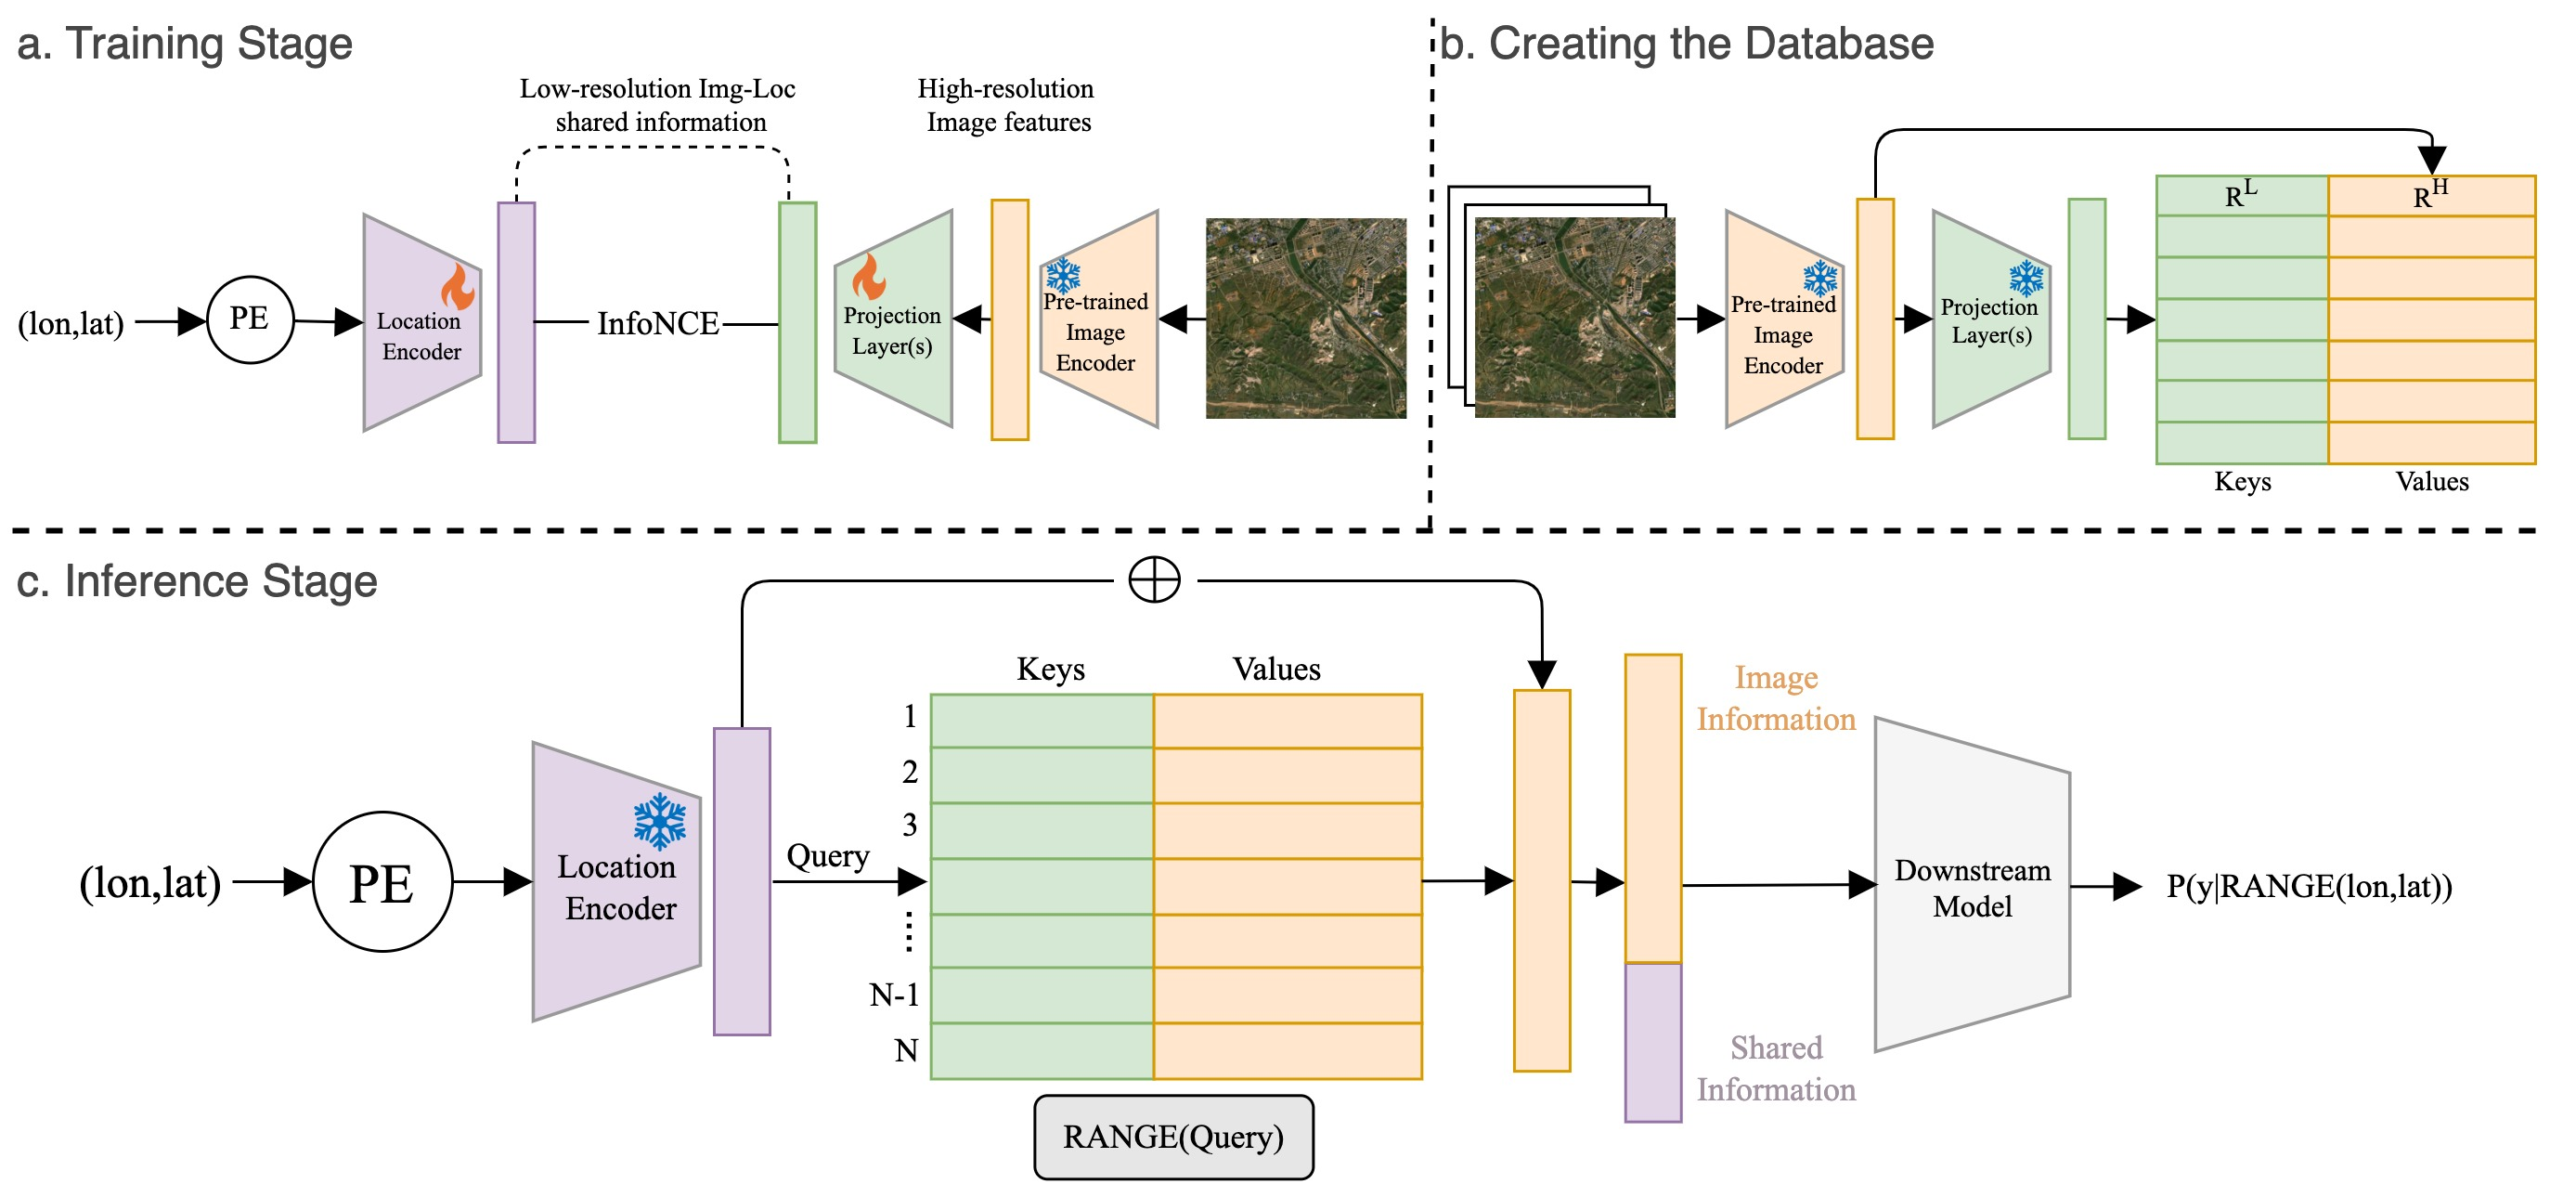
\includegraphics[width=\linewidth, scale=0.3]{proposal/images/framework_cam.jpg}
\end{center}
    \caption{Framework of RANGE. (a) In the training stage, a shared embedding space is learned between locations and images. (b) We create a database of low-resolution and high-resolution image embeddings using the trained projection layer and a powerful pretrained image model, respectively. (c) During inference, we use a location as the query, low-resolution image embeddings as keys, and high-resolution image embeddings as values. Using our retriever function, we compute the approximate high-resolution embeddings for the query. We concatenate ($\oplus$) the approximated visual feature with our query embedding.} 
\label{fig:framework}
\end{figure*}
\subsection{Aligning Location and Image is a Multi-View Non-Redundancy Problem}
\label{sec:multi-view}
Let (L,H,T) represent location modality, image modality, and geospatial task, respectively. Models like SatCLIP and GeoCLIP align co-located images and locations by minimizing the infoNCE objective. Solving the multimodal infoNCE objective maximizes the lower bound on the mutual information, preserving the shared information within the learned representations~\cite{oord2018representation}. As such, the final learned representations of these models contain only information that is shared across both location and image. This property is useful under the multi-view redundancy assumption, which states that the information shared between the two modalities is exactly relevant to solve the underlying task~\cite{tosh2021contrastive}. However, this assumption does not hold in the location-image learning setting, as there is high unique information contained in the image modality that is useful for solving downstream tasks. Formally, we argue that location-image learning falls under the multi-view non-redundancy setting: there is \textit{unique} information in the image modality that is not shared with the location modality, and that information is relevant for solving our geospatial task T. In this case, contrastive training discards valuable task-relevant information from the image, leading to poor downstream performance~\cite{liang2023factorized}.

\subsection{Method}
\label{sec:range-method}
We consider a dataset with paired geolocations and co-located satellite images $\{g_i, s_i\}$. The goal is to learn a meaningful representation for $g_i$ by aligning it with $s_i$, which can be done by minimizing the clip objective \cite{klemmer2023satclip, vivanco2024geoclip, radford2021learning}. We have a trainable geolocation encoder $E$, a frozen pretrained image encoder $I$, and a projection layer $P$. Let $G_i = E(g_i)$ represent the location embedding, $S_i = {I(s_i)}$ represent the frozen image embedding, and $P_i = P(I(s_i))=P(S_i)$ represent the image embedding obtained from the projection layer for the i$^{th}$ sample. We minimize the objective:
%
\begin{align}
&L_{i}^{loc} = \frac{-1}{k}\sum_{i=1}^{k} \log\frac{\exp(G_i \cdot P_i / \tau)}{\sum_{j=1}^{k} \exp(G_i \cdot P_j) / \tau) } \\
&L_{i}^{img} = \frac{-1}{k}\sum_{i=1}^{k} \log\frac{\exp(G_i \cdot P_i / \tau)}{\sum_{j=1}^{k} \exp(G_j \cdot P_i) / \tau) } \\
&L_i = (L_i^{loc} + L_i^{img})/2 
\end{align}
%
The training process is shown in Figure~\ref{fig:framework}-(a). We contrastively align the geolocations and satellite images by minimizing their CLIP objective. This formulation is identical to SatCLIP~\cite{klemmer2023satclip}, so we use the pretrained SatCLIP image and location encoders for simplicity. For query location $g_i$, $S_i$ encodes the high-resolution visual features since $I$ is a powerful pre-trained image encoder. Both $P_i$ and $G_i$ encode low-resolution shared information between $g_i$ and $s_i$. The resulting geo-embedding, $G_i$, is sub-optimal as it loses unique visual information crucial for many downstream tasks. To solve this, we propose a retriever function $R_\tau$ that allows us to approximate the high-resolution information $S_i$ given $g_i$. Let $\epsilon$ denote the deviation from the true visual embedding. We can then explicitly add the approximate visual information $\hat{S_i}$ to our location embedding $G_i$:
    \begin{align}
    &R_\tau(g_i) = \hat{S_i} = S_i + \epsilon \\
    &RANGE(g_i) = \hat{S_i} \oplus G_i 
    \end{align}

\begin{table}
\centering    

% \hspace*{-1.3cm}
\resizebox{\linewidth}{!}{
\begin{tabular}{l|ccc|ccccc}
\hline
                        & Biome & EcoRegions & Country   & Temperature & Elevation & Population & Cali-Housing   \\ \hline
Direct                      & 29.1 & 0.6 & 66.9& 0.381  & 0.025  &  0.053  & 0.238      \\
Cartesian\_3D                      & 30.2 & 1.8 &66.9 & 0.362  & 0.030  &  0.162  & 0.240      \\
Wrap~\cite{Aodha_2019_ICCV}                      & 34.4 & 1.1 & 69.7& 0.861  & 0.085  &  0.328  & 0.239      \\
Theory~\cite{gaolearning}                      & 33.5 & 1.0 &72.5 & 0.849  & 0.093  &  0.330  & 0.254      \\
SphereM~\cite{mai2023sphere2vec}                      & 36.4 & 27.3 & 72.7 & 0.629  & 0.139  &  0.302  & 0.423      \\
SphereM$^{+}$~\cite{mai2023sphere2vec}                      & 58.7 & 50.1 & 76.1 & 0.886  & 0.294  &  0.421  & 0.543      \\
SphereC~\cite{mai2023sphere2vec}                     & 36.3 & 52.9 & 72.9 & 0.461  & 0.185  &  0.335  & 0.496      \\
SphereC$^+$~\cite{mai2023sphere2vec}  & 53.2 & 61.6 & 73.6 & 0.842  & 0.260  &  0.392  & \underline{0.544}      \\

\hline


CSP-INat~\cite{mai2023csp}                      & 61.1 & 57.1 & 75.9 & 0.717  & 0.388  &  0.554  & 0.462      \\
CSP-FMoW~\cite{mai2023csp}                    & 61.4 & 58.0 & 81.3& 0.865  & 0.399  &  0.580  & 0.541      \\
SINR~\cite{cole2023spatial}                    & 67.9 & 54.9 & 88.3 & \textbf{0.942}  & 0.644  & 0.726 & 0.420      \\
GeoCLIP~\cite{vivanco2024geoclip}                & \underline{70.2} & 71.6 & 81.3 & 0.916  &  0.604  &  0.698  & \textbf{0.708}      \\
SatCLIP~\cite{klemmer2023satclip}  & 68.9 & 69.3 & 82.8 & 0.825       & 0.666     & 0.684 & 0.400   \\ \hline


RANGE  & \textbf{83.3} & \textbf{75.7} & \underline{93.7} &0.895 & \underline{0.844} & \underline{0.799} & 0.422  \\ 


RANGE$^+$                      & \textbf{83.3} & \underline{75.3} & \textbf{94.7} &\underline{0.931} & \textbf{0.851} & \textbf{0.811} & 0.336 &    \\ 
\end{tabular}
}
\caption{Our model shows improvements over a variety of tasks compared to state-of-the-art models. The first 3 columns are classification tasks with accuracy metrics and the last 4 columns are regression tasks with R$^2$ metric. We show improvements with significant margins across many of the tasks. Our model underperforms in the Cali-housing dataset. We further analyze this behavior in our discussions.}
\label{table:main}
\end{table}

\subsubsection{Retrieval Augmented Neural Fields}
\noindent \textbf{Creating the Retrieval Database: }Once the contrastive training is done, we create a retrieval database as shown in Figure~\ref{fig:framework}-(b). We take $\{g_i, s_i\}$ sampled uniformly across the globe using the SatCLIP~\cite{klemmer2023satclip} dataset. For every location $g_i$ in our data, we compute: a) the shared-information image embedding $R_i{^L}=P(I(s_i))$, and b) the high-resolution image embedding $R_i{^H}=\bar{I}(s_i))$; we refer to these sets of embeddings as low-resolution embeddings and high-resolution embeddings, respectively, in the rest of the paper. In practice, $\bar{I}$ can differ from $I$; the only condition is that $\bar{I}$ is a pretrained image feature extractor. For our purposes, we use SatMAE~\cite{cong2022satmae} as $\bar{I}$. 
\\
\\
\noindent \textbf{Retriever Function: }
Let $R^L=\{R_{1}^L, R_{2}^L,...R_{N}^L\}$, and $R^H=\{R_{1}^H, R_{2}^H,...R_{N}^H\}$ represent the set of all low-resolution and high-resolution image embeddings in our database. After creating the database, we need a method to sample appropriate high-resolution image information for a query location. Naively, we can set this as a lookup operation, where $G_i$ is the query, $R^L$ is the set of all keys, and $R^H$ is the set of all values. We have a function $sim(G_i, R_{j}^{L})$, which gives the alignment scores between i and j. In our setting, this similarity function is a simple cosine similarity. For a query $G_i$, we find $R_{j}^{L}$ with the highest alignment score and return the key $R_{j}^{H}$. 
In practice, $R_{j}^{H}$ is noisy. The semantically closest image in the database can contain additional information that is irrelevant to the location. Therefore, naively adding $R_{j}^{H}$ has the potential of introducing incorrect information to our geo-embeddings. 



We instead use a soft selection criteria. First, we compute the query's alignment score with each key in the database using cosine similarity. We use a softmax function to convert the alignment scores to probabilities. We also use a temperature parameter $\tau$ to slightly reshape the probability distribution; $\tau$ is extremely robust as it does not need to be fine-tuned for different tasks or for databases with different distributions. We use the resulting probabilities to compute a weighted average across all values, i.e., high-resolution image embeddings in the database. The resulting embedding is an approximation of $S_i$, where the information contributed by each image is weighted by its alignment score with the query. We concatenate this approximate high-resolution image embedding with our original location embedding $G_i$ to obtain the multi-resolution RANGE embedding $RANGE_i$. A high-level view of this process is shown in Figure~\ref{fig:framework}-(c). 

\begin{equation}
    RANGE_i = R_{\tau}(G_i) \oplus G_i 
= \frac{1}{N}\sum_{k=1}^{N}{\frac{e^{sim(G_i,R_{k}^L)/\tau}}
{\sum_{j=1}^{N}{e^{sim(G_i,R_{j}^L)/\tau}}}} * R_{k}^H \oplus G_i
\end{equation}
\noindent $\text{, where}\ G_i\in \mathbb{R}^M,\ R_{k}^L \in \mathbb{R}^M,\ R_{k}^H \in \mathbb{R}^{N}.$
%
\\
\\
\noindent \textbf{Adding smoothness constraints: }We also propose another version of our model called $RANGE^+$. Here, we additionally use geodesic similarity to approximate the visual features of the location. We convert our query location to 3D cartesian coordinates and use angular distance to find the spatially closest image in the database. This spatial retrieval allows us to impose spatial smoothness on our embeddings since locations close to each other are forced to have similar retrieval, irrespective of the semantics.  The spatially retrieved embedding is added to the semantically retrieved embedding and weighted using a $\beta$ parameter, which controls the level of spatial smoothness enforced on the $RANGE$ embeddings. Let $g{_i}^{3D}$ be the query location, $l$ be the set of all database locations in 3D cartesian coordinates, and $sim(g{_i}^{3D}, l_k)$ be their angular similarity:   
\begin{multline}
\label{eq:rangep}
RANGE^+_{i} = \frac{1}{N}(\beta*\sum_{k=1}^{N}{\frac{e^{sim(G_i,R_{k}^L)/\tau_{1}}}{\sum_{j=1}^{N}{e^{sim(G_i,R_{j}^L)/\tau_{1}}}}} * R_{k}^H+ \\ 
     (1-\beta)\sum_{k=1}^{N}{\frac{e^{sim(g{_i}^{3D},l_{k})/\tau_{2}}}{\sum_{j=1}^{N}{e^{sim(g{_i}^{3D},l_{j})/\tau_{2}}}}} * R_{k}^H
     )\oplus G_i \\
\end{multline}
$\text{, where } G_i \in \mathbb{R}^M, \ g{_i}^{3D} \in \mathbb{R}^3, \ l_k \in \mathbb{R}^3$
\begin{table}[]
\centering
\begin{tabular}{l|c|ccccc}
\textbf{} & $\beta$ & \begin{tabular}[c]{@{}c@{}}100\\ \footnotesize 19.21$^\circ$\end{tabular} & \begin{tabular}[c]{@{}c@{}}500\\ \footnotesize 8.72$^\circ$\end{tabular} & \begin{tabular}[c]{@{}c@{}}1000\\ \footnotesize 6.11$^\circ$\end{tabular} & \begin{tabular}[c]{@{}c@{}}1500\\ \footnotesize 5.06$^\circ$\end{tabular} & \begin{tabular}[c]{@{}c@{}}2000\\ \footnotesize 4.34$^\circ$\end{tabular} \\ \hline

SatCLIP &  & 36.0 & 26.4 & 25.5 & 25.5 & 21.7 \\
GeoCLIP &  & 64.1 & 22.8 & 15.7 & 14.4 & 13.8 \\
CSP-INat &  & 44.9 & 27.1 & 24.0 & 21.9 & 18.5 \\
CSP &  & 67.8 & 33.8 & 26.8 & 23.9 & 21.1 \\
SINR &  & 87.6 & 58.4 & 34.3 & 22.6 & 19.0 \\
\hline
 & 0       & \textbf{94.0}                                                                            & \textbf{73.2}                                                                           & 50.0                                                                                     & 43.1                                                                                     & 37.8                                                                                     \\
          & 0.25    & \underline{93.3}                                                                               & \underline{72.6}                                                                              & \underline{55.8}                                                                               & 50.7                                                                                     & 45.3                                                                                     \\
   RANGE$^+$       & 0.5     & 92.3                                                                                     & 70.0                                                                                    & \textbf{56.4}                                                                            & \textbf{52.3}                                                                            & \textbf{47.2}                                                                            \\
          & 0.75    & 89.4                                                                                     & 65.1                                                                                    & 54.5                                                                                     & \underline {50.6}                                                                               & \underline {46.3}                                                                               \\
          & 1       & 65.7                                                                                     & 53.6                                                                                    & 50.5                                                                                     & 46.6                                                                                     & 42.6                                                                                    
\end{tabular}
\caption{We quantitatively show that controlling the beta parameter allows us to generate optimal embeddings depending on the resolution of the task. We evaluate on the checkerboard task~\cite{russwurm2023geographic} and change the number of grid cells in the Fibonacci lattice to simulate tasks with different spatial resolutions. Lower $\beta$ yields better embeddings for low-resolution tasks, whereas higher $\beta$ yields better embeddings for high-resolution tasks. We see that we outperform all the baselines across all spatial resolutions.}
\label{table:beta}

\end{table}
\subsection{Results}
\subsubsection{Quantitative Evaluation on Downstream Tasks}
We evaluate the efficacy of RANGE and RANGE$^+$ embeddings on a wide variety of downstream applications. We choose 3 classification tasks (biome, ecoregion, and country classification) and 4 regression tasks (population density estimation, temperature, elevation, and housing price prediction) for this experiment, as used by prior work~\cite{klemmer2023satclip}. We compare our method with SoTA parametric~\cite{klemmer2023satclip, vivanco2024geoclip, cole2023spatial, mai2023csp, mai2023sphere2vec} and non-parametric~\cite{Aodha_2019_ICCV,gaolearning} representations. The results of this experiment are shown in Table~\ref{table:main}. The results show that our method outperforms all state-of-the-art models in the classification tasks with significant margins. Among the regression tasks, we achieve SoTA performance for elevation and population density prediction with significant gains and narrowly come second in the air temperature prediction task. Furthermore, RANGE$^+$, on average, outperforms RANGE by a small margin, which can be attributed to the spatial smoothness constraint.

\begin{figure*}[!t]
\begin{center}
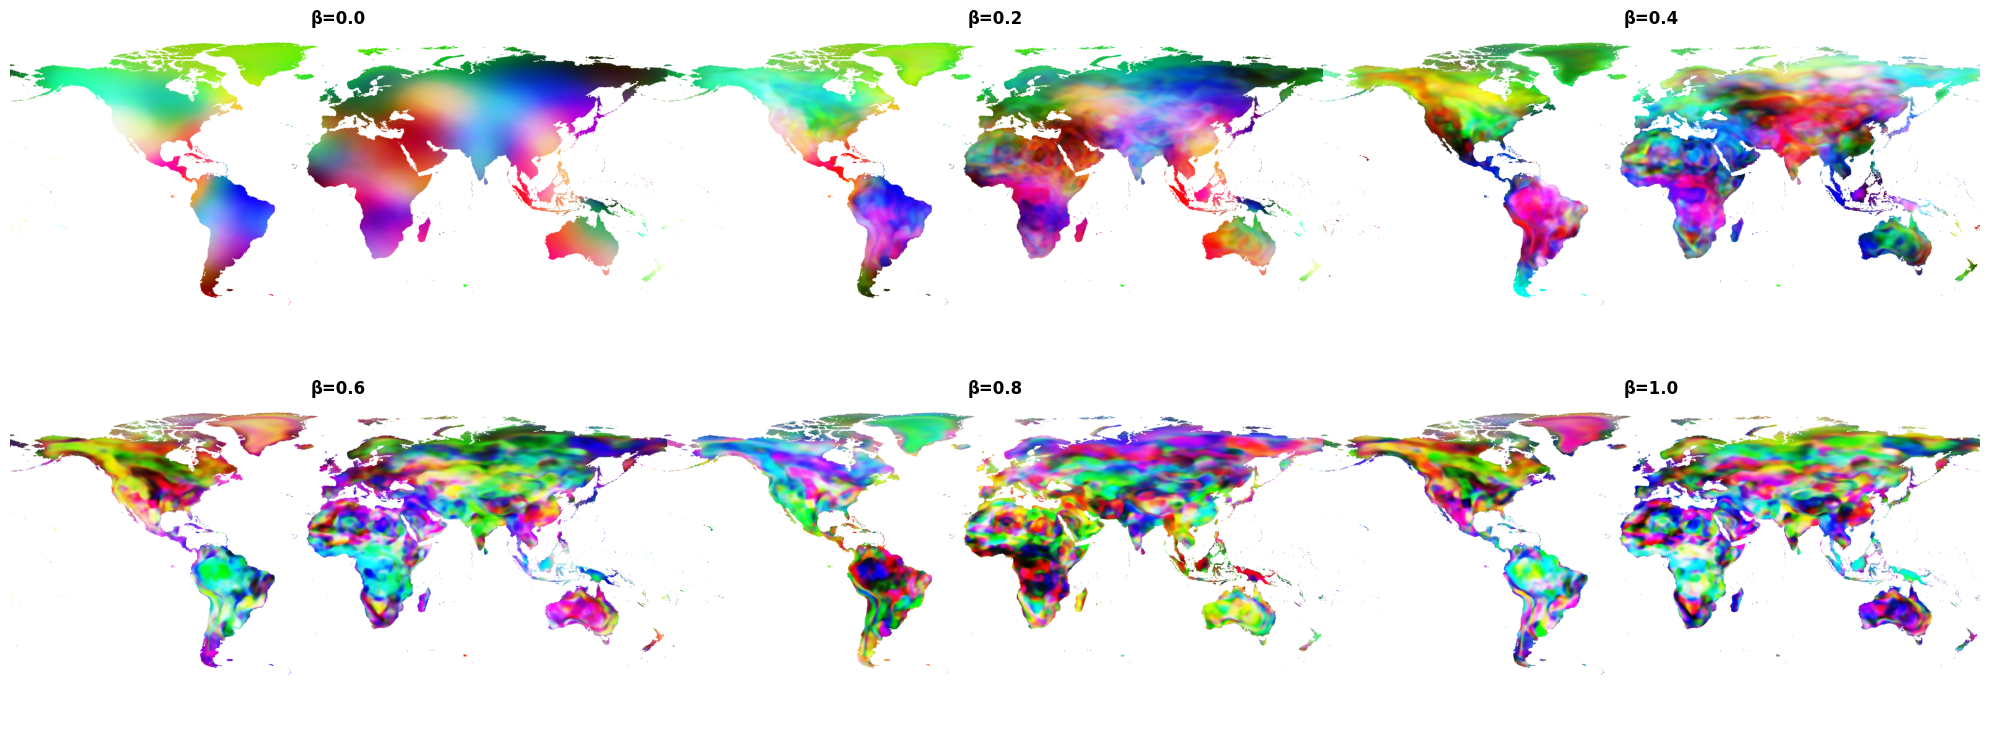
\includegraphics[width=\linewidth, scale=0.3]{proposal/images/beta_interpolation_2.png}
\end{center}
   \caption{Interpolating the $\beta$ parameter in RANGE$^+$ allows us to control the spatial smoothness of our embeddings. The results show that RANGE$^+$ can be used to generate neural fields of geo-embeddings at multiple frequencies.} 
\label{fig:beta}
\end{figure*}

\subsubsection{Understanding the Impact of $\beta$ parameter}
We attempt to understand the impact of the $\beta$ parameter in equation~\eqref{eq:rangep}. First, we perform a quantitative evaluation of varying $\beta$. Our results in Table~\ref{table:beta} show that a lower beta is optimal for low-resolution tasks, whereas a higher beta is usually better for high-resolution tasks. We also compute the ICA of the embeddings at different $\beta$ and plot them over the map of the world to qualitatively assess the differences. The results in Figure~\ref{fig:beta} show that
RANGE+ can be used to generate neural fields of geo-embeddings at multiple frequencies. 

\subsection{Proposed Direction}
We showed the utility of RANGE embeddings across a large number of downstream tasks such as population density estimation, biome prediction, fine-grained species classification etc. However, all our evaluations were limited to discriminative tasks. We will work towards understanding the utility of our general purpose neural field for solving generative tasks. Specifically, we will use RANGE embeddings to improve existing geospatial generative models. Geospatial generative models try to generate realistic looking satellite images. Our RANGE embeddings contain high-resolution information, and conditioning the generative models using these embeddings can enable improved location conditioned generation.   

\subsection{Chapter Conclusion}
In this chapter, we proposed a new framework for general purpose neural field over the earth. We showed the limitations of directly adapting generic representation learning methods for geospatial data. Specifically, we showed that using contrastive training for geolocation representation learning violates assumptions of multi-view redundancy, resulting in sub-optimal representations. We proposed a retrieval-augmented strategy for estimating visual features from an auxiliary database of visual embeddings. Our approach results in significant improvements for a variety of tasks as compared to purely parametric embedding strategies with only a modest increase in storage requirements. Hence, we highlighted the importance of designing data-specific representation learning strategies and understanding the assumptions and limitations of existing approaches. 
\section{Chapter 2: Learning a Neural Field of Text Representations using Satellite Images}
\label{sec:sat2cap}
Dhakal, Aayush, et al. ``Sat2cap: Mapping fine-grained textual descriptions from satellite images." \textit{IEEE/ISPRS Workshop: Large Scale Computer Vision for Remote Sensing (Best Paper EARTHVISION) 2024.}
\subsection{Overview}
In the previous chapter, we proposed a framework to learn a general-purpose neural field over the earth. In this chapter, we will learn a specialized neural field of text-aligned representations. For any location $(lat,lon)$, we want to learn a function $R= F_\theta(lat,lon)$, where $R$ captures the fine-grained text describing the query location. Instead of directly using the geolocation coordinates as input to the neural field, we use a satellite image as a proxy for the location, i.e., $ R = F_\theta(Img(lat, lon))$.

Modeling the relationship between text and images is a well-studied problem in deep learning. Models such as CLIP~\cite{radford2021learning} and ALBEF~\cite{li2021align} are trained on a large database of captioned images to learn a multimodal embedding space that unifies vision and text. However, we observe that directly using these models on satellite imagery leads to the collapse of representations into a few coarse textual concepts, such as city, beach, and island. Satellite images capture a broad perspective of a geolocation but offer limited insight
into the intricate concepts and dynamics within the location. Hence, directly using overhead images with such models would only allow us to learn coarse-level textual concepts.

One solution is to train a model using satellite images and fine-grained captions of those locations. However, such datasets do not exist in large-scale. To address this issues, we exploit the cross-view relation of satellite images with corresponding ground-level images. Specifically, we propose a weakly-supervised
cross-view approach for learning fine-grained textual concepts for geographic locations by leveraging co-located ground-level images. We create a large-scale dataset with paired overhead and ground-level images. We then train a model that aligns overhead images with ground-level images in the CLIP space. Our training leverages an emergent behaviour, where aligning the overhead images with ground-level images, as a by-product, aligns them with the corresponding text descriptions of the ground-level images. This allows us to learn a fine-grained vision-language representation space for satellite images in the absence of text data.  

\begin{equation}
    G_i = f_\theta{(g_i)}
\end{equation}
\begin{equation}
    O_i = g_\theta{(o_i)}
\end{equation}    

To align the overhead image embeddings with the ground-level CLIP embeddings, we contrastively train our model using the InfoNCE~\cite{oord2018representation} loss as follows:
%
\begin{equation}
    L = \frac{1}{k}\sum_{i=0}^{k} -\log\frac{exp(O_i \cdot G_i / \tau)}{\sum_{j=0}^{k} exp(O_i \cdot G_j / \tau) }
\end{equation}

\begin{figure*}[!t]
\begin{center}
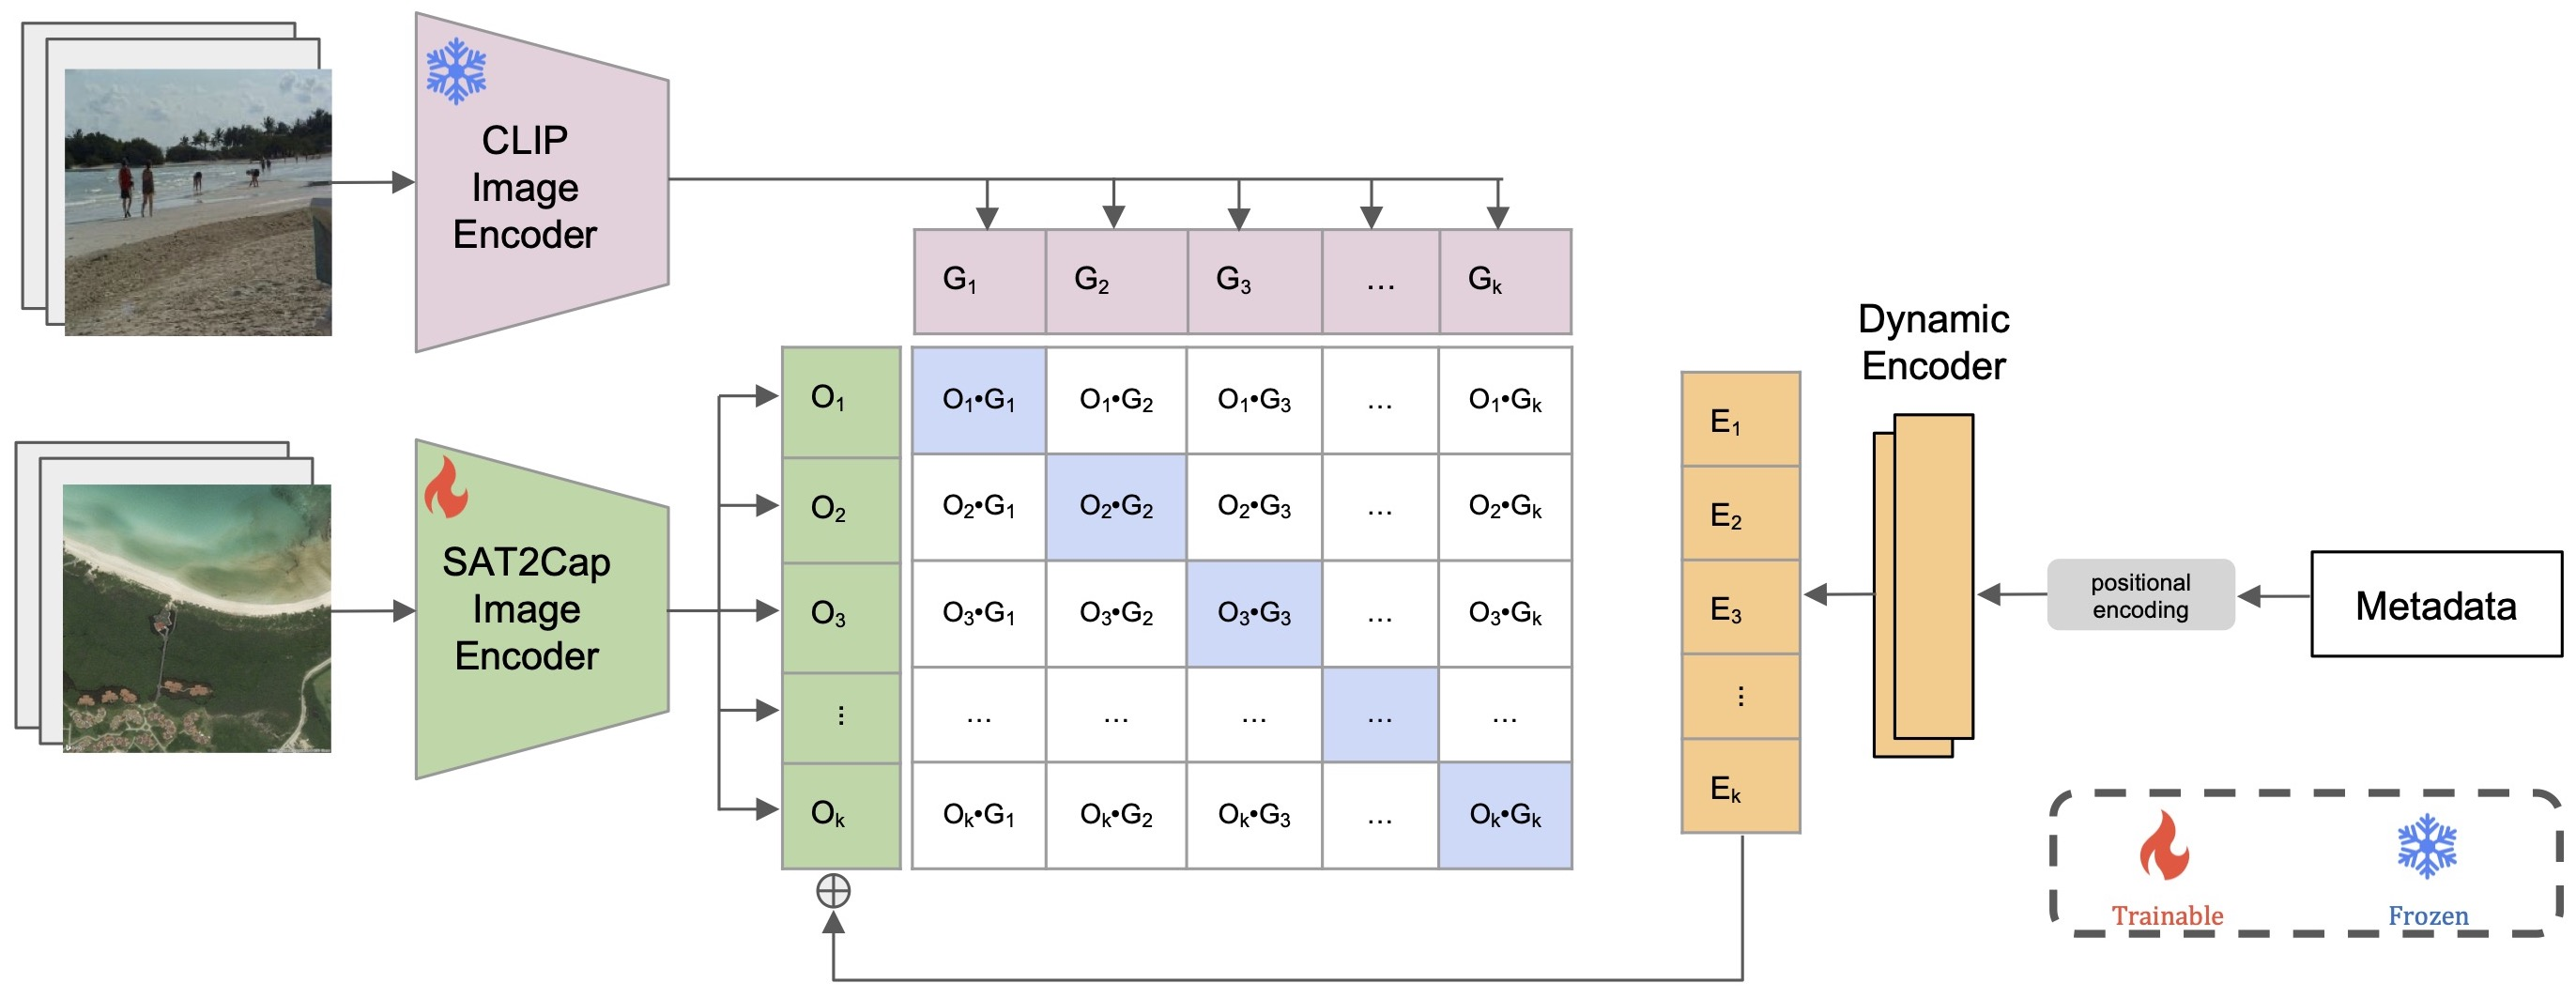
\includegraphics[width=\linewidth, scale=0.3]{proposal/images/framework.jpg}
\end{center}
   \caption{\textbf{Sat2Cap Framework:} The frozen CLIP Image Encoder takes as input the ground-level images and generates their CLIP embeddings. The trainable Sat2Cap Image Encoder takes as input the overhead images, and the Dynamic Encoder takes as input the date, time, and location information. The respective overhead image embeddings and meta-information embeddings are added element-wise, and the resulting embeddings are contrastively trained with the CLIP embeddings of the ground-level images.}  
\label{fig:Sat2Cap}
\end{figure*}
\subsection{Method}
\label{sec:method}
Our objective is to learn an embedding space that describes the expected ground-level scene given a geographic location and an overhead image. We have ground-level images $\{g_1, g_2, ...g_n\}$, corresponding overhead images $\{o_1, o_2, ...o_n\}$, and respective metadata for the ground-level images $\{e_1, e_2, ...e_n\}$. Each $e_i$ contains the latitude and longitude information of the sample, as well as the date and time for when the ground-level image was captured. We also have a CLIP image encoder $f_{\theta}$ that generates CLIP embeddings for a given ground-level image.

\subsubsection{Dataset}
\label{dataset}
We created a large-scale cross-view dataset to train our model. The ground-level images in the dataset are taken from the YFCC100M~\cite{thomee2016yfcc100m} dataset. The YFCC100M dataset contains 99.3 million images, which are collected from Flickr. Our cross-view dataset uses a smaller sample from this collection which excludes all US imagery. We filter out all images that are not geotagged. The resulting dataset contains 6.1M images. Each of these images has a geolocation, timestamp, and other meta-information. For each image, we download an overhead image centered at its location. Specifically, we use the Bing Maps API to download $800$x$800$ patch satellite images at $0.6m/px$ resolution. We randomly sampled 100k images to be used for testing.

\newcommand{\cmark}{\ding{51}}%
\newcommand{\xmark}{\ding{55}}%

\begin{table}
 \begin{center}
 \small
 \resizebox{\linewidth}{!}{
    \begin{tabular}{c c c c |c c c|c c c}
 \hline
 \multicolumn{4}{c|}{Method} &
 \multicolumn{3}{c|}{Overhead2Ground (10K)} &
 \multicolumn{3}{c}{Ground2Overhead (10K)} \\
 
 \hline
 Model &Meta/Training &Dropout & Meta/Inference & R@5$\uparrow$ & R@10$\uparrow$ & Median-R$\downarrow$ & R@5$\uparrow$ & R@10$\uparrow$ & Median-R$\downarrow$\\
 \hline
 CLIP & - &- & - & 0.007 & 0.013 & 1700 & 0.108 & 0.019 & 2857 \\
 \hline
 \multirow{4}{2em}{ours} & \xmark & \xmark & \xmark & 0.398 & 0.493 & 15 & 0.356 & 0.450 & 11\\
 & \cmark & \xmark & \xmark & 0.322 & 0.413 & 34 & 0.254 & 0.343 & 20\\
 & \cmark& \xmark & \cmark & 0.368 & 0.467 & 23 & 0.298 & 0.398 & 13\\
 & \cmark& \cmark & \xmark & 0.467 & 0.564 & 13.5 & 0.366 & 0.462 & 7\\
 & \cmark& \cmark & \cmark & \textbf{0.493} & \textbf{0.591} & \textbf{12} & \textbf{0.390} & \textbf{0.482} & \textbf{6}\\


\end{tabular}
}
\end{center}
  \caption{\textbf{Cross-view retrieval performance of Sat2Cap model:} The table shows that CLIP performs poorly for the task of cross-view retrieval. Moreover, we study the performance of our model under various settings. The \textbf{Meta/Training} column ablates the impact of adding meta-information in training. The \textbf{Dropout} column ablates the impact of randomly dropping out the Dynamic Encoder in training. The \textbf{Meta/Inference} column ablates the impact of adding meta-information in inference. Our experiments show that using all three achieves the best performance.}
\label{table:retrieval}
\end{table}

\subsubsection{Approach}
We initialize our Sat2Cap image encoder $g_\theta$ with the weights of $f_\theta$. A batch of ground-level images $\{g_1, g_2, ..., g_k\}$ is passed through the CLIP encoder to get the ground-level CLIP embeddings. These embeddings serve as the target for alignment. A batch of corresponding overhead images $\{o_1, o_2, ..., o_k\}$ is passed through the Sat2Cap image encoder to obtain the respective embeddings:  
%
We also keep a queue $Q$ and fill it with CLIP embeddings of ground images. Here, $|Q|>>k$ and the embeddings from the queue are used as additional negative samples for our contrastive objective. As in MoCo~\cite{he2020momentum}, the queue is continuously updated during the training with the most recent batch. Minimizing this objective minimizes the distance between co-located overhead and ground-level images in the CLIP space. It is worth noting that throughout the training process, the CLIP image encoder is frozen. Hence, with our training procedure, we allow the overhead images to move close to images from their respective ground-level scene in the CLIP space. As a byproduct, the overhead images also move closer to the textual descriptions of ground-level images, which we are ultimately interested in mapping.

\begin{figure*}[!t]
\begin{center}
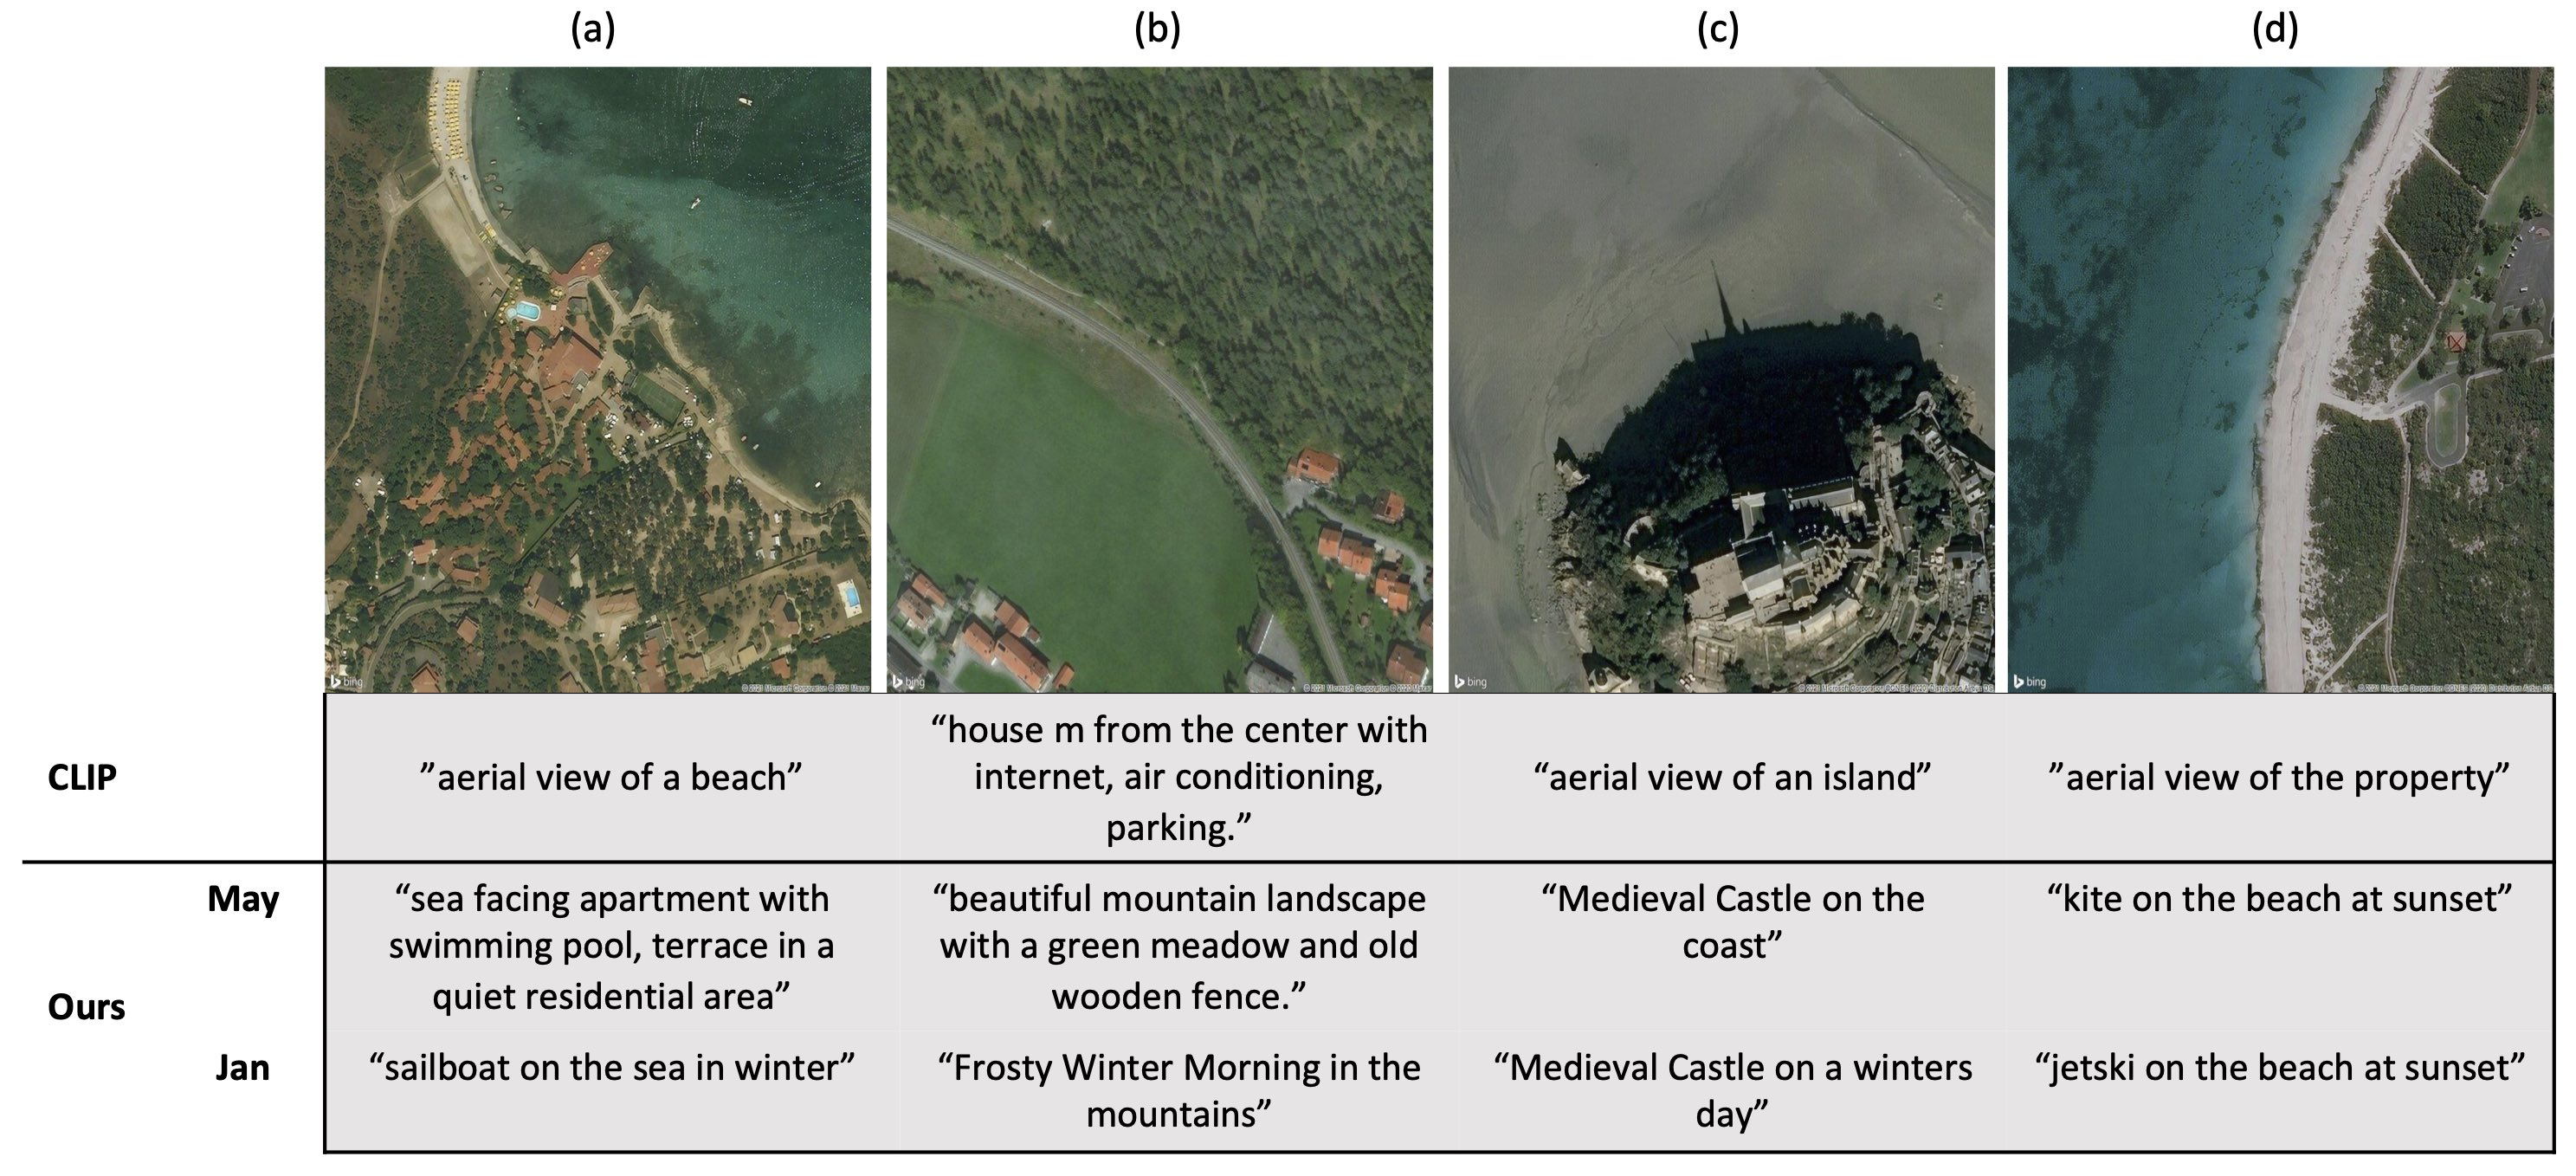
\includegraphics[width=0.95\linewidth]{proposal/images/caption_gen_2.jpg}
\end{center}
   \caption{Captions generated by the CLIPCAP model \cite{mokady2021clipcap} using CLIP embeddings vs.\ Dynamic Sat2Cap embeddings. (Row-1) shows the results from CLIP embeddings, which produce many generic descriptions. (Row-2 and 3) show the results from our Sat2Cap embeddings for the month of May and January, respectively. The captions generated using Sat2Cap embeddings are more fine-grained and dynamic. While (d) does not add any winter properties for the January query, this behavior is expected as the image is over Australia, where January falls in the middle of summer.}    
\label{fig:img1}
\end{figure*}

\begin{figure*}[!t]
    \centering
    % First subfigure
    \begin{subfigure}{}
        \centering
        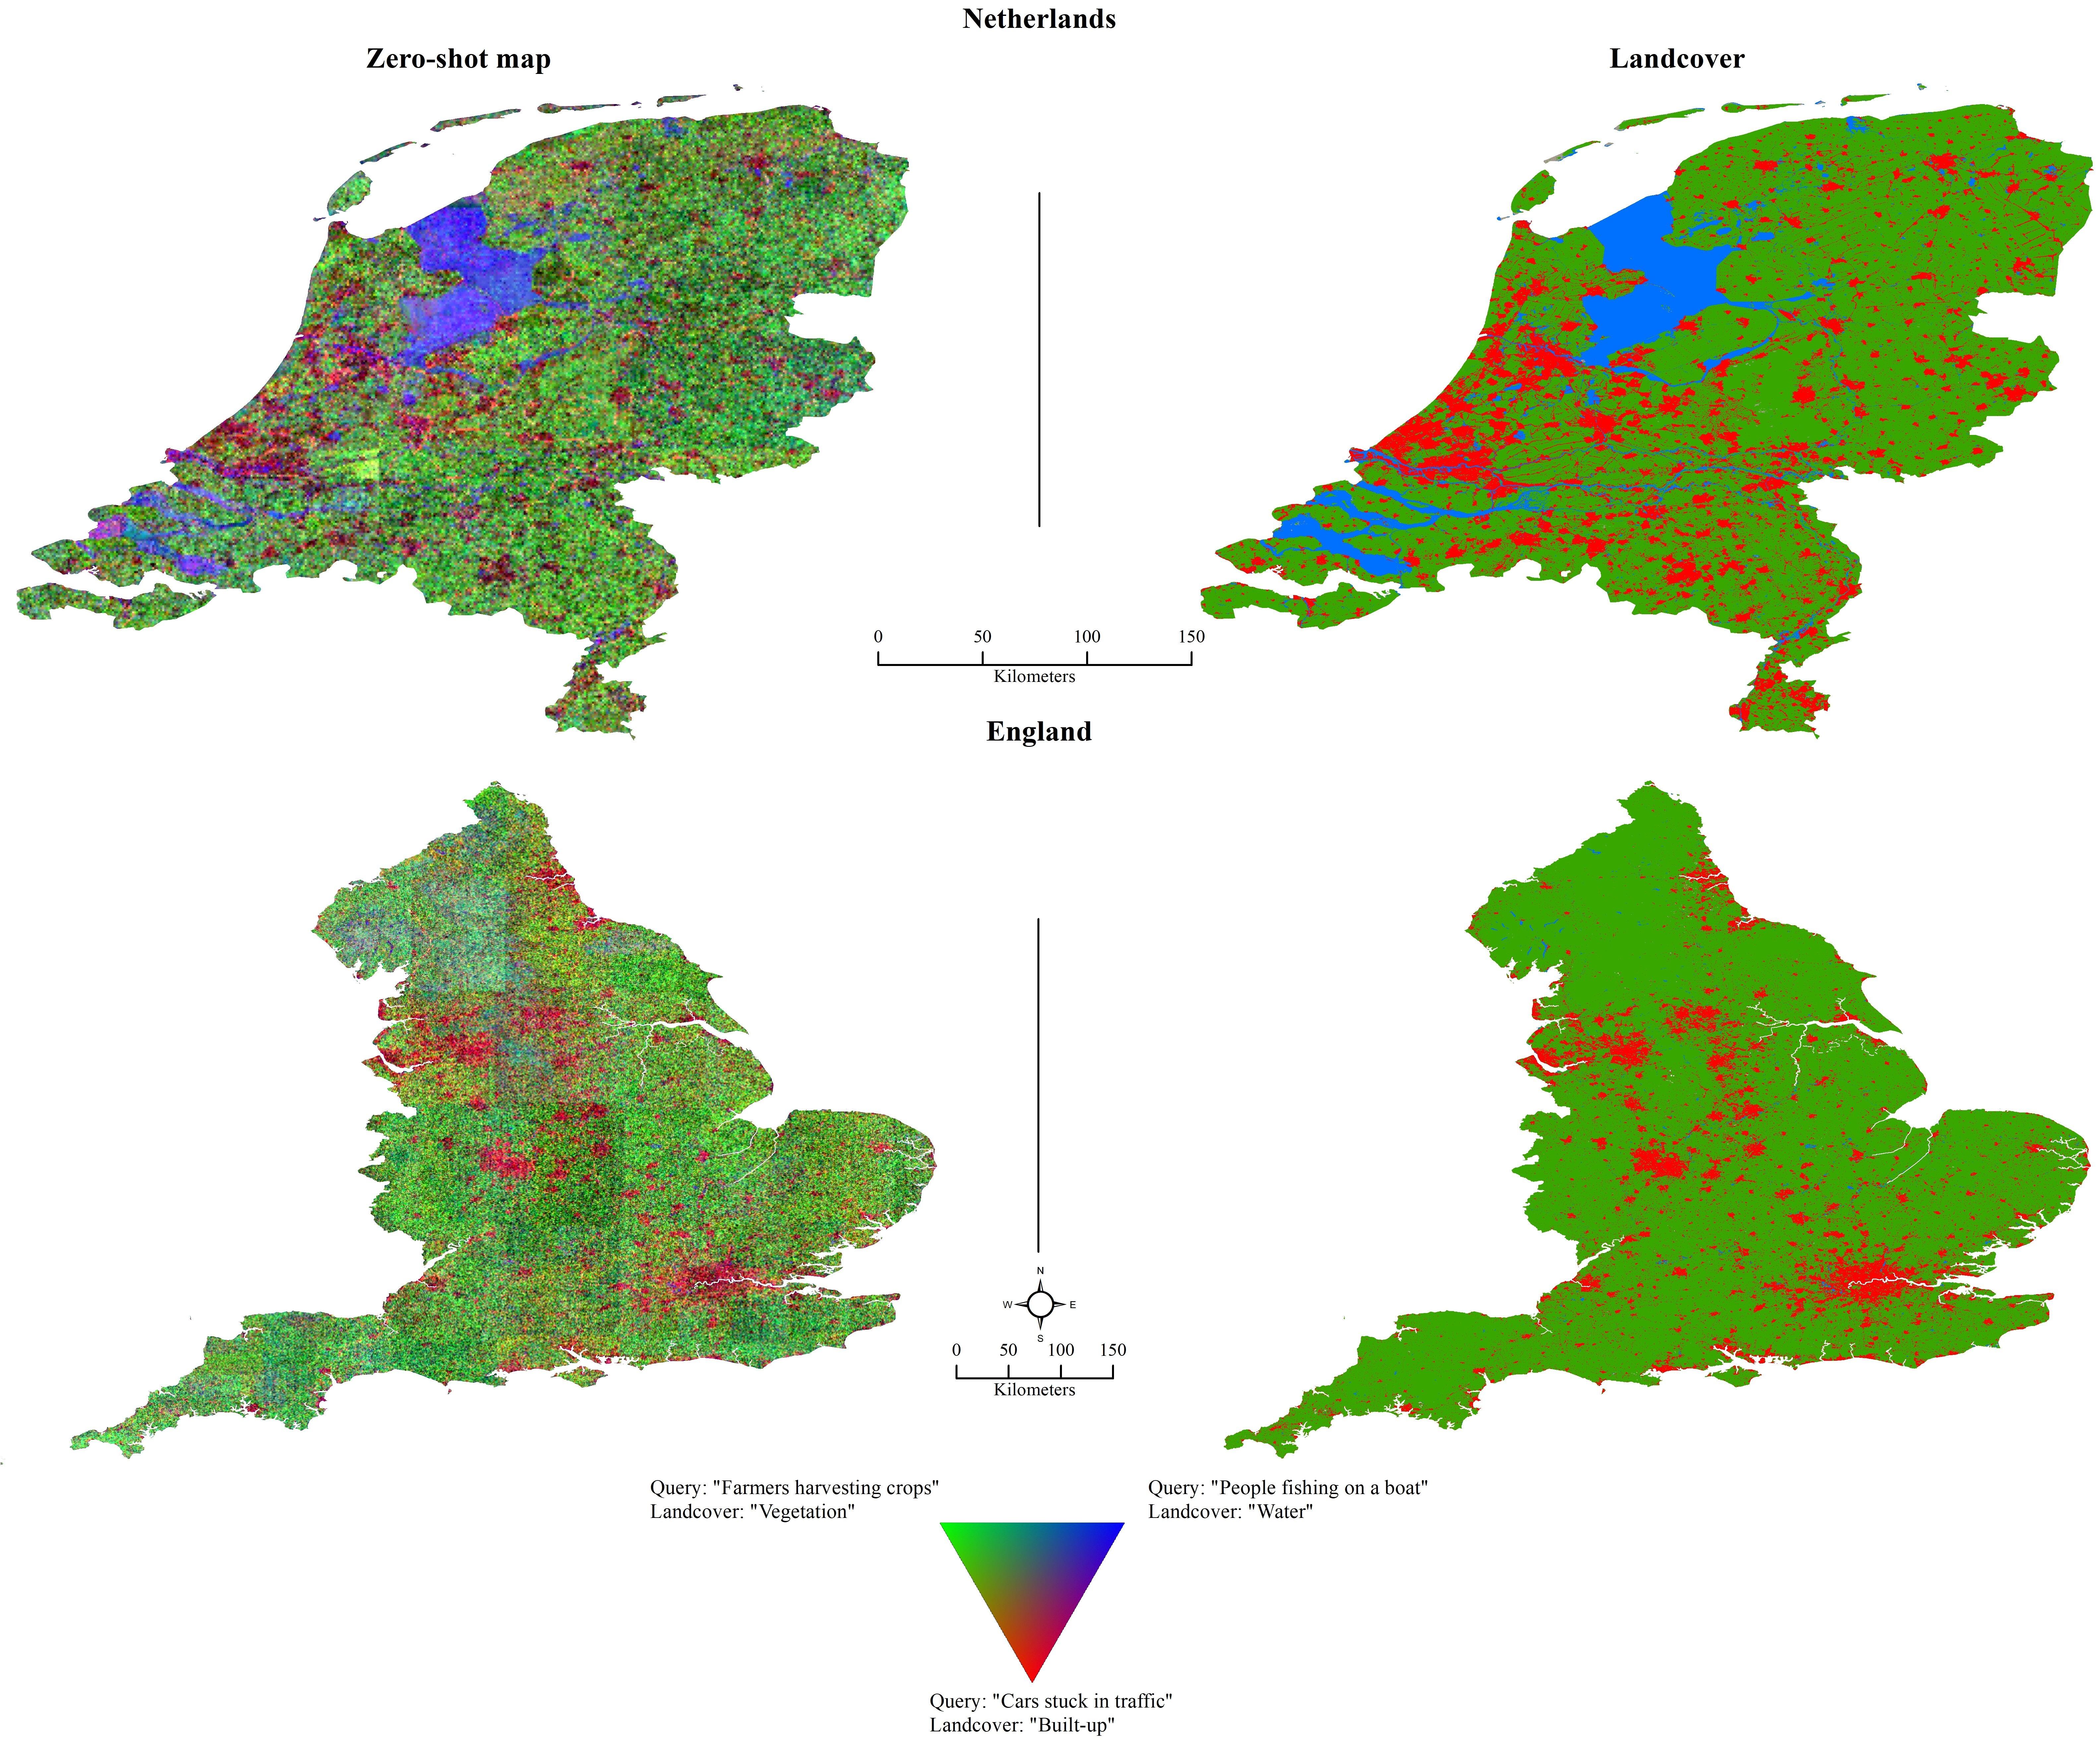
\includegraphics[width=\linewidth,height=0.5\textheight,keepaspectratio]{proposal/images/rgb_map.jpg}
        \caption{\textbf{Country-level maps of textual descriptions}: (Col 1-2) shows the country-level maps created using Sat2Cap for three prompts: ``Cars stuck in traffic," ``People fishing on a boat," and ``Farmers harvesting crops." We compare the predicted zero-shot maps with landcover maps of the region.}
        \label{fig:generic_maps}
    \end{subfigure}
    \vskip 0.5em
    % Second subfigure
    \begin{subfigure}{}
        \centering
        \includegraphics[width=\linewidth,height=0.4\textheight,keepaspectratio]{proposal/images/ams_road.jpg}
        \caption{\textbf{Fine-grained maps CLIP vs Sat2Cap:} We create zero-shot maps on a city level using CLIP and Sat2Cap for two prompts: ``Heavy trucks transporting goods" and ``People waking in the streets of downtown." Compared to CLIP, Sat2Cap activations are more localized to the appropriate regions for a given prompt. Sat2Cap is better at distinguishing between fine-grained concepts like \textbf{highway} and \textbf{downtown street}.}
        \label{fig:fg_maps}
    \end{subfigure}
    \label{fig:maps_combined}
\end{figure*}
\subsubsection{Learning Dynamic Concepts of Places}

Many ground-level concepts are temporally dependent. Concepts like ``crowded street", or ``snowy place" can dramatically vary based on the exact time we query about them. To model such dynamic concepts, we condition Sat2Cap on the timestamps of the ground-level images.

For each sample, we extract the year, month, day, and hour in which the ground image was taken. We also add the geolocation information to provide a stronger signal to the model. We encode this meta-information using sin-cos encoding and pass it through a shallow, fully connected network, which we call the Dynamic Encoder $(h_\theta)$. The output from $h_\theta$ is added element-wise to the output from the Sat2Cap encoder before computing the objective.

\begin{equation}
    S_i = O_i + E_i
\end{equation}
where $O_i$ is the output from the Dynamic Encoder. Now the objective function changes to:
\begin{equation}
\label{eq:finaleq}
   L_{dynamic} = \frac{1}{k}\sum_{i=0}^{k} -\log\frac{exp(S_i \cdot G_i / \tau)}{\sum_{j=0}^{k} exp(S_i \cdot G_j / \tau) } 
\end{equation}
where $S_i$ is the sum of outputs from the Image Encoder and Dynamic Encoder 

Our complete framework is shown in Figure~\ref{fig:Sat2Cap}. To prevent overfitting to the meta-information, we implement random dropout of the Dynamic Encoder during training. Our experiments from Section~\ref{sec:sat2cap_results} show that this addition significantly improves the performance of our model.

\subsection{Results}
\label{sec:sat2cap_results}
Our model learns a powerful geo-text embedding space that can be used for a variety of applications. We describe three experiments to demonstrate the efficacy of our model.
\subsubsection{Cross-View Image Retrieval}
In this experiment, we show that our model learns a strong relationship between co-located overhead images and ground images in the CLIP space. We randomly sample 10,000 image pairs from the test set for this experiment. First, we predict the Sat2Cap embeddings for all overhead images and the corresponding CLIP embeddings for all the ground-level images in the test set. We then compute top-k (or R@k) and median rank metrics between the Sat2Cap overhead embeddings and the CLIP ground embeddings. The top-k metric measures how often the ground truth falls within the top-k closest images for a given query image. Table~\ref{table:retrieval} shows the cross-view retrieval results.

Our results highlight that CLIP space, in itself, is remarkably poor at learning the relationship between a location and the corresponding ground-level scene. The low cross-view retrieval scores imply that we cannot accurately reason about ground-level scene using the CLIP embeddings of co-located overhead images. On the other hand,  the high cross-view retrieval scores of Sat2Cap suggest that the Sat2Cap embedding of a location approximates the CLIP embeddings of the images at the ground-level. This ultimately results in an emergent alignment between location and textual descriptions of the ground level.
\subsubsection{Fine-grained and Dynamic Caption Generation}
To generate captions from our embeddings, we use the CLIPCap~\cite{mokady2021clipcap} model. CLIPCap allows us to generate captions by learning a mapping from the CLIP space to the text space. Figure~\ref{fig:img1} shows qualitative examples of captions generated by passing CLIP embedings vs Sat2Cap embeddings as input for a given overhead image. We observe that when using CLIP embeddings of the overhead images as input, the captions generated by CLIPCap mostly describe generic concepts of a location like a beach, island, property, etc. In contrast, our Sat2Cap embeddings produce more fine-grained and aesthetically pleasing captions. Furthermore, we use the dynamic encoder to generate captions in two different months, for the same location.

\subsubsection{Zero-Shot Map of Fine-grained Concepts}
We use Sat2Cap embeddings to create zero-shot maps using fine-grained prompts. To do this, we choose a region and download high-resolution satellite images $(0.6m/px)$ over the region. We precompute the Sat2Cap embeddings for all the images. At inference time, for a given text query, we predict the CLIP embedding and compute its similarity with the overhead image embeddings. The process of computing the similarities only takes about 4 seconds. Figure~\ref{fig:generic_maps} and Figure~\ref{fig:fg_maps} show zero-shot maps at country-scale and city-scale data.

\subsection{Proposed Direction}
We are also working on follow-up of Sat2Cap. Sat2Cap leveraged pre-trained vision-language models to learn the correspondence between satellite images and ground-level image descriptions. One key limitation of this approach is that it learns a single ground-level concept/embedding/descriptor for a given satellite image, resulting in coarse-grained information. We are currently working on Sat360, a framework that learns the correspondence between satellite image and ground-level image descriptions conditioned on a viewing direction. More specifically, Sat360 allows learning fine-grained text for specific regions within a satellite image, which was not possible using Sat2Cap. Our key insight is that explicitly aligning viewing orientation by pairing directional crops from street view panoramas with their corresponding masked regions in overhead imagery, achieves pixel-level correspondence without manual annotations. By leveraging the joint vision-language space, Sat360 enables zero-shot tasks such as fine-grained cross-view retrieval, orientation estimation, and open-vocabulary aerial segmentation. We are currently working on Sat360 and plan to submit a paper on November. 

\subsection{Chapter Conclusion}
In this chapter, we proposed a specialized neural field of textual representations. We presented a weakly supervised framework for learning a semantically rich embedding space between geolocation and fine-grained text. For this task, we leveraged the unique property of satellite images i.e. relation of satellite images with corresponding ground-level images. By leveraging this property, we were able to learn a foundational vision-language model without using any text. We demonstrated that our framework can efficiently generate high-quality zero-shot maps from fine-grained text prompts. Thus, we demonstrated that it is possible to develop efficient learning algorithms, by understanding the unique properties of the input modality and incorporating those insights into our models. 



\section{Chapter 3: Understanding the Risks and Benefits of Generative Models from the Perspective of Representation Learning}

\subsection{Overview}
In the first two chapters, we explore how powerful representations of data allow us to solve downstream tasks with greater efficiency and efficacy. We posed the geospatial representation learning problem as a neural field problem where we want to learn $R=F_\theta(lat, lon)$. Generative models pose a double-edged role in this landscape. On the positive side, they can be used to expand datasets through synthetic augmentation and unlock new possibilities for representation learning. The efficacy of representation learning scales with data and generative models can provide an easy alternative to scale pretraining. However, generative models also introduce the risk of contaminating training pipelines with low-quality data. Such contamination can mislead models into capturing spurious correlations, amplify existing biases, and ultimately yield representations that diverge from the true structure of the data. From this perspective, generative models are not simply tools for data creation but also potential vectors for introducing noise, bias, and adversarial artifacts into our neural representation fields. Understanding and mitigating these risks is, therefore, essential for building trustworthy and robust downstream models.

In Chapter 3, we will examine the potential risks and limitations of deep-generative geospatial models. First, we will demonstrate that current generative geospatial models introduce strong artifacts in the generated images. Second, we will propose a new metric that measures the strength of these artifacts in a given generative model. Third, we present SimLBR, a simple and efficient solution for detecting fake images in a real-world black-box setting, where the source of an image is unknown. SimLBR learns a tight decision boundary around the real image distribution using latent blending regularization, and generalizes to unseen generators on both natural-image and satellite-image benchmarks. We further extend SimLBR with structured latent blending strategies that improve its reliability on the hardest, most out-of-distribution generators. Finally, we will use the findings to propose better generative models that can feed into representation learning pipelines while maintaining the integrity and fidelity of the learned representations. By doing so, we aim to ensure that generative augmentation enhances rather than compromises the quality of downstream tasks, paving the way for robust, trustworthy, and scalable geospatial AI systems.

\subsection{Do Geospatial Generative Models Introduce Strong Artifacts in their Images?}
\label{sec:few-shot}
In this section, we will examine various geospatial generative models and assess the quality of the generated fakes. We will do this by using few-shot learning. Images that exhibit strong artifacts will be easier to detect compared to images that do not contain such artifacts. Hence, it should be possible to learn a good deepfake detector for models with strong artifacts, even when we only have access to a few samples.
\\
\\
\noindent \textbf{Dataset:}
We will use the RSFAKE-1M data, a large-scale dataset for detecting diffusion-generated remote sensing forgeries~\cite{tan2025rsfake}. The dataset contains 500,000 real and 500,000 forged satellite images. The forged images are obtained from 10 different diffusion models that are trained on remote sensing images. 
\\
\\
\noindent\textbf{Experimental Setup:} 
Assume we have real images from set $R$, and fake images from set $F$. All images in $F$ are generated from the same model. We want to understand if it is possible to identify all samples in $F$, if we only have access to a subset of $F$, $G$ with n fake images during training (where n is very small).

During training, we have access to $R=\{r_1, r_2, ..., r_k\}$, and $G=\{g_1, g_2, ...g_n\}$. All the real images are passed through a powerful, pre-trained satellite image encoder $I$, which produces the set of real features $R_f$. Since $\lvert R \lvert >> \lvert G \lvert$, we apply multiple augmentations to $g_i$, and artificially increase the number of fake samples. All of the fake samples are then passed through the pre-trained satellite image encoder $I$, which produces the set of generated image features $G_f$. We then train a simple linear binary classifier to distinguish between real and fake images.
\\
\\
\begin{table*}[]
\resizebox{\linewidth}{!}{
\begin{tabular}{llll|lll|lll|lll}
\multicolumn{1}{r}{} & \multicolumn{3}{c|}{100 samples} & \multicolumn{3}{c|}{10 samples} & \multicolumn{3}{c|}{2 samples} & \multicolumn{3}{c}{1 sample} \\ \hline
                     & Acc   & Auc   & \multicolumn{1}{l|}{F1} & Acc   & Auc   & \multicolumn{1}{l|}{F1} & Acc   & Auc   & \multicolumn{1}{l|}{F1} & Acc   & Auc   & F1 \\ \hline
Geosynth         & 0.999 & 0.999 & 0.999 & 0.998 & 0.999 & 0.998 & 0.979 & 0.997 & 0.979 & 0.969 & 0.995 & 0.969 \\
Geosynth-SAM     & 0.999 & 0.999 & 0.999 & 0.997 & 0.999 & 0.997 & 0.986 & 0.999 & 0.986 &    0.986   &    0.999   &   0.986   \\
Rsinpaint        & 0.969 & 0.997 & 0.969 & 0.931 & 0.986 & 0.928 & 0.877 & 0.964 & 0.863 & 0.775 & 0.908 & 0.725 \\
GeoRSSD (fmow)       & 0.997 & 0.999 & 0.997 & 0.992 & 0.999 & 0.992 & 0.988 & 0.999 & 0.988 & 0.979 & 0.998 & 0.979 \\
MapSat           & 0.999 & 0.999 & 0.999 & 0.996 & 0.999 & 0.996 & 0.995 & 0.999 & 0.995 & 0.845 & 0.979 & 0.819 \\
DiffusionSat-512 (fmow) & 0.994 & 0.999 & 0.994 & 0.986 & 0.999 & 0.985 & 0.943 & 0.991 & 0.941 & 0.890 & 0.976 & 0.881 \\
DiffusionSat-256 (fmow) & 0.995 & 0.999 & 0.995 & 0.989 & 0.999 & 0.989 & 0.967 & 0.994 & 0.967 & 0.854 & 0.967 & 0.836 \\
CrsDiff (fmow) & 0.997 & 0.999 & 0.997 & 0.968 & 0.997 & 0.968 & 0.908 & 0.989 & 0.900 & 0.606 & 0.831 & 0.368 \\
SDFRS            & 0.999 & 0.999 & 0.999 & 0.999 & 0.999 & 0.999 & 0.978 & 0.998 & 0.977 & 0.982 & 0.999 & 0.981 \\


\end{tabular}
}
\caption{A linear classifier with few-shot examples yields good results in detecting geospatial deepfakes.}
\label{table:few-shot}
\end{table*}
\noindent\textbf{Preliminary Results:}
We conduct this experiment for each model in the RSFAKE-1M dataset. We report the results for $n=\{100,10,2,1\}$. The results are reported in Table~\ref{table:few-shot}. The preliminary results show that it is possible to learn a strong binary classifier with access to as few as one fake sample from a generative model. This leads us to make two crucial hypotheses:
\begin{enumerate}
    \item Every image generated from a model contains artifacts that are, in part or in whole, shared by any other images generated from the same model.
    \item Including images with such strong artifacts for training new models will result in biased models and biased representations.
\end{enumerate}
We will design methods to validate these hypotheses experimentally.

\subsection{A New Metric to Understand the Presence of Artifacts in Geospatial Deepfakes}
\label{sec:seperability}
Based on our findings in Section~\ref{sec:few-shot}, we will propose a new metric to measure the performance of a geospatial generative model. Our metric measures, ``for a generative model $G$, how many randomly-sampled fake images are needed to learn a linear classifier that gets an accuracy of K on an unseen test set". The linear classifier is learned using the protocol described in Section~\ref{sec:few-shot}. When comparing different models, the same feature extractor must be used for a fair comparison. For a generative model, a lower value of Separability indicates that the model introduces trivial artifacts in all images that it produces. In contrast, a higher value suggests that artifacts are less prevalent. We will compute the Separability value for the state-of-the-art generative models to have a better understanding of which models can be used to generate synthetic data with minimal risks. 

\subsection{SimLBR: Learning to Detect Fake Images by Learning to Detect Real Images}
\label{sec:simlbr}
The few-shot experiments in Section~\ref{sec:few-shot} show that a detector can be trained to recognize the fakes of a \textit{known} generator from only a handful of samples. In practice, however, the source of an image is unknown, and the generator that produced a fake image may not have existed when the detector was trained. While it is relatively easy to train a detector that performs well on fakes produced by a specific generative model, real-world deployment demands detectors that generalize to unseen and more advanced generators~\cite{ojha2023towards,yansanity,zhong2023patchcraft}. Unfortunately, most existing detectors overfit, learning superficial cues that are specific to the training generator rather than generalizable differences between real and fake images, and their performance collapses on images synthesized by novel generators. In this section, we present SimLBR~\cite{dhakal2026simlbr}, a simple and efficient framework for generalizable fake image detection using Latent Blending Regularization (LBR). Although our motivation comes from geospatial generative models, the problem of cross-generator generalization is not specific to satellite imagery. We therefore develop and evaluate SimLBR on standard natural-image benchmarks, and additionally evaluate it on the RSFake-1M benchmark of generated satellite images~\cite{tan2025rsfake}.

\noindent\textbf{From SimDLR to SimLBR:}
Our preliminary formulation of this idea, SimDLR, aimed to prevent overfitting by \textit{diversifying the artifacts} seen during training: each fake embedding was linearly combined with the embedding of another randomly sampled real or fake image, and the combination was labeled as fake. While this improved cross-generator generalization on RSFake-1M, it still asks the detector to model the \textit{fake} distribution, which is a moving target. In SimLBR, we reverse the role of the two classes. Instead of enlarging the region of the latent space that is covered by fake samples, we perturb \textit{real} samples with small amounts of fake information and label them as fake. This forces the detector to learn a tight decision boundary around the real image distribution and to treat the fake category as a sink class. The rest of this section describes this formulation in detail.

\begin{figure}[!t]
\centering
\begin{minipage}[t]{0.48\linewidth}
  \centering
  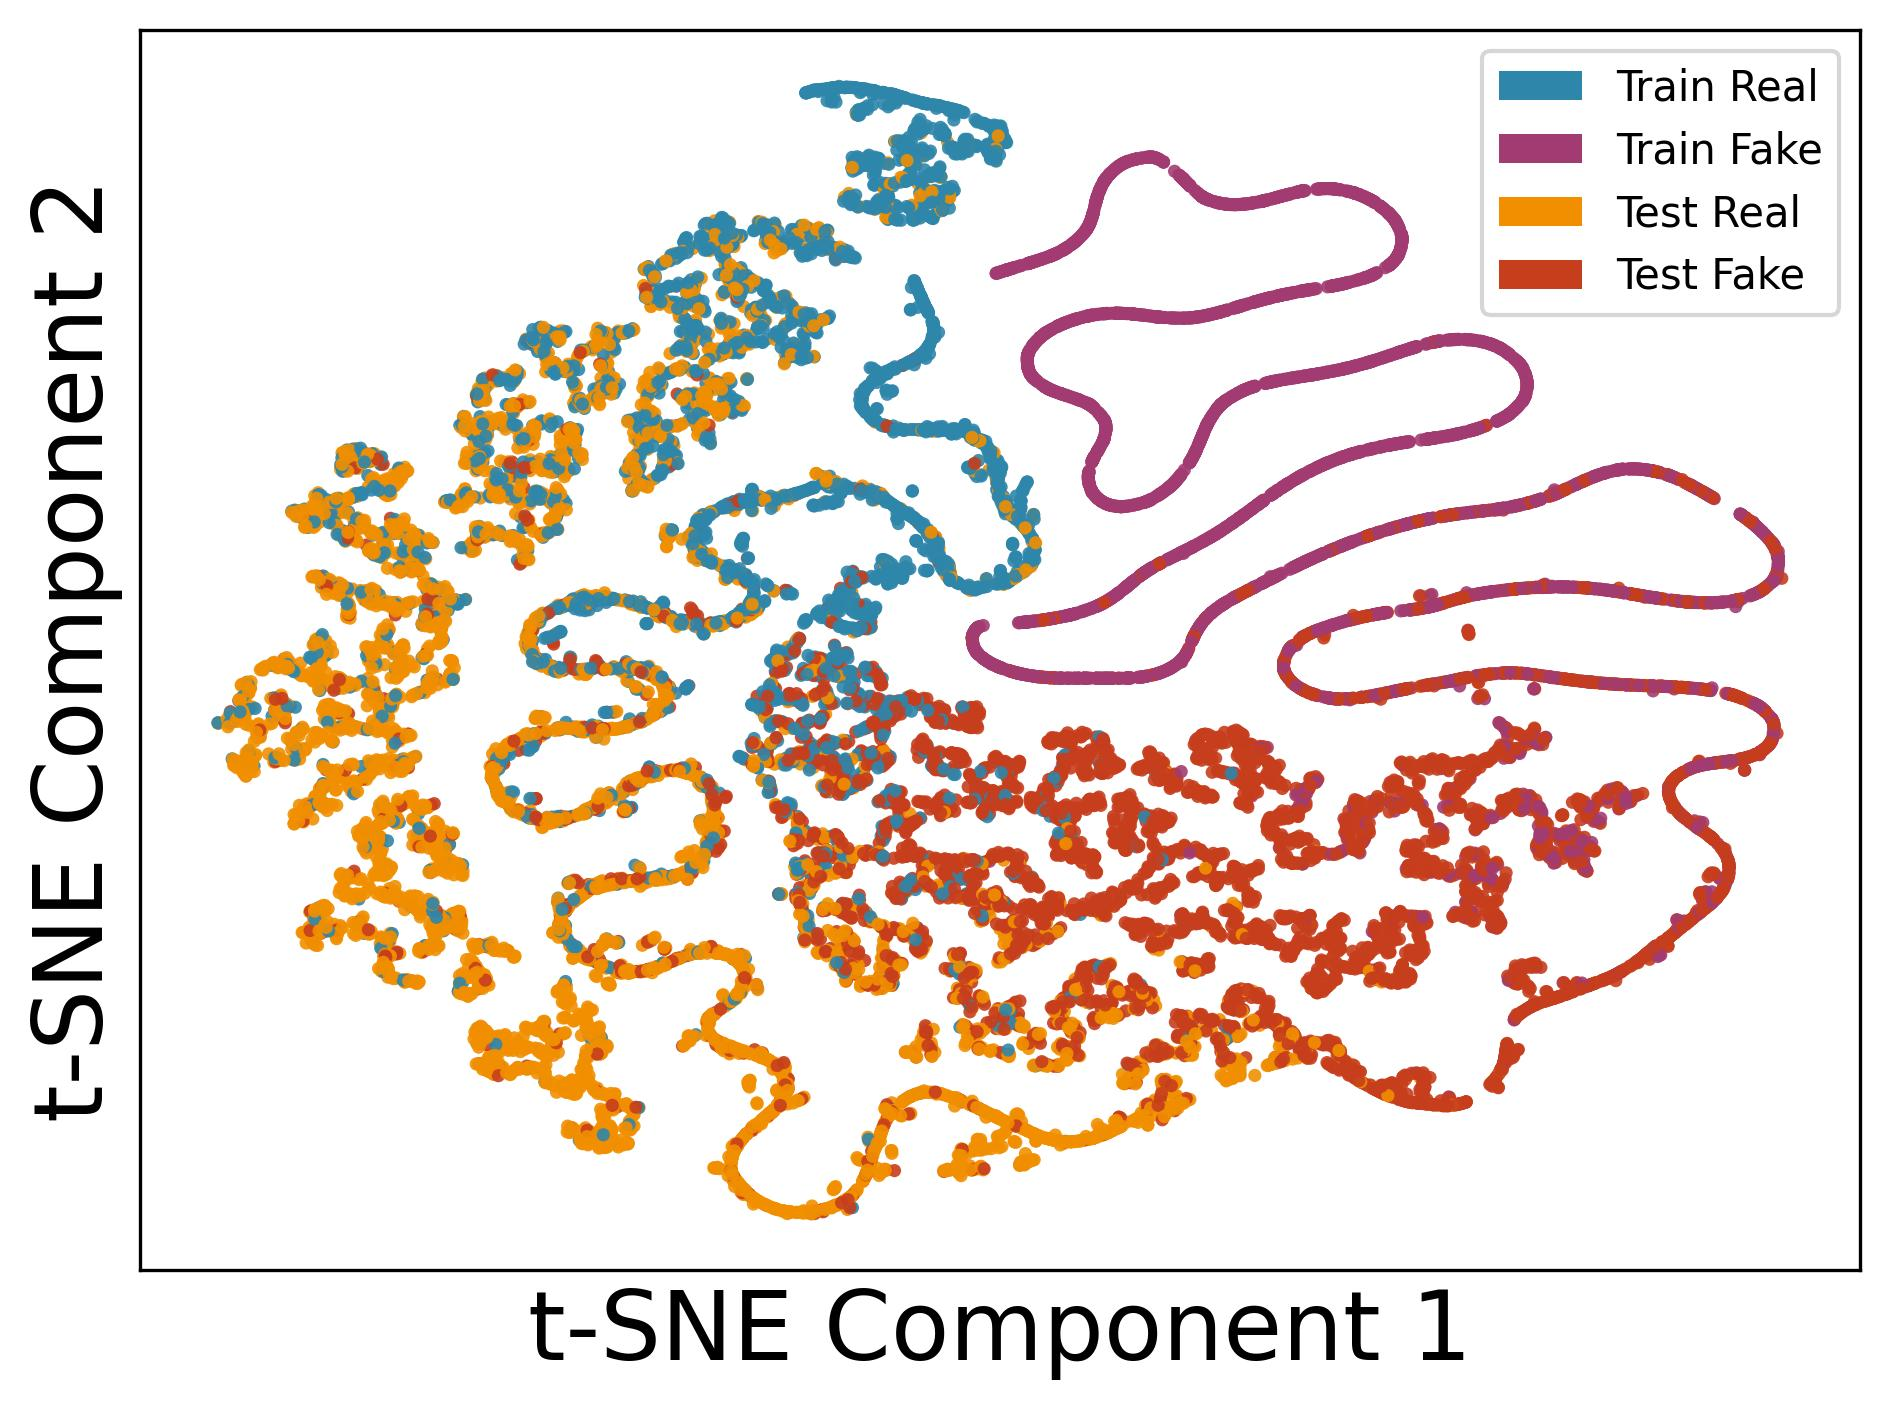
\includegraphics[width=\linewidth]{proposal/images/simlbr/tsne_wo_lbr_wukong.jpeg}\\
  {\small (a) w/o LBR}
\end{minipage}\hfill
\begin{minipage}[t]{0.48\linewidth}
  \centering
  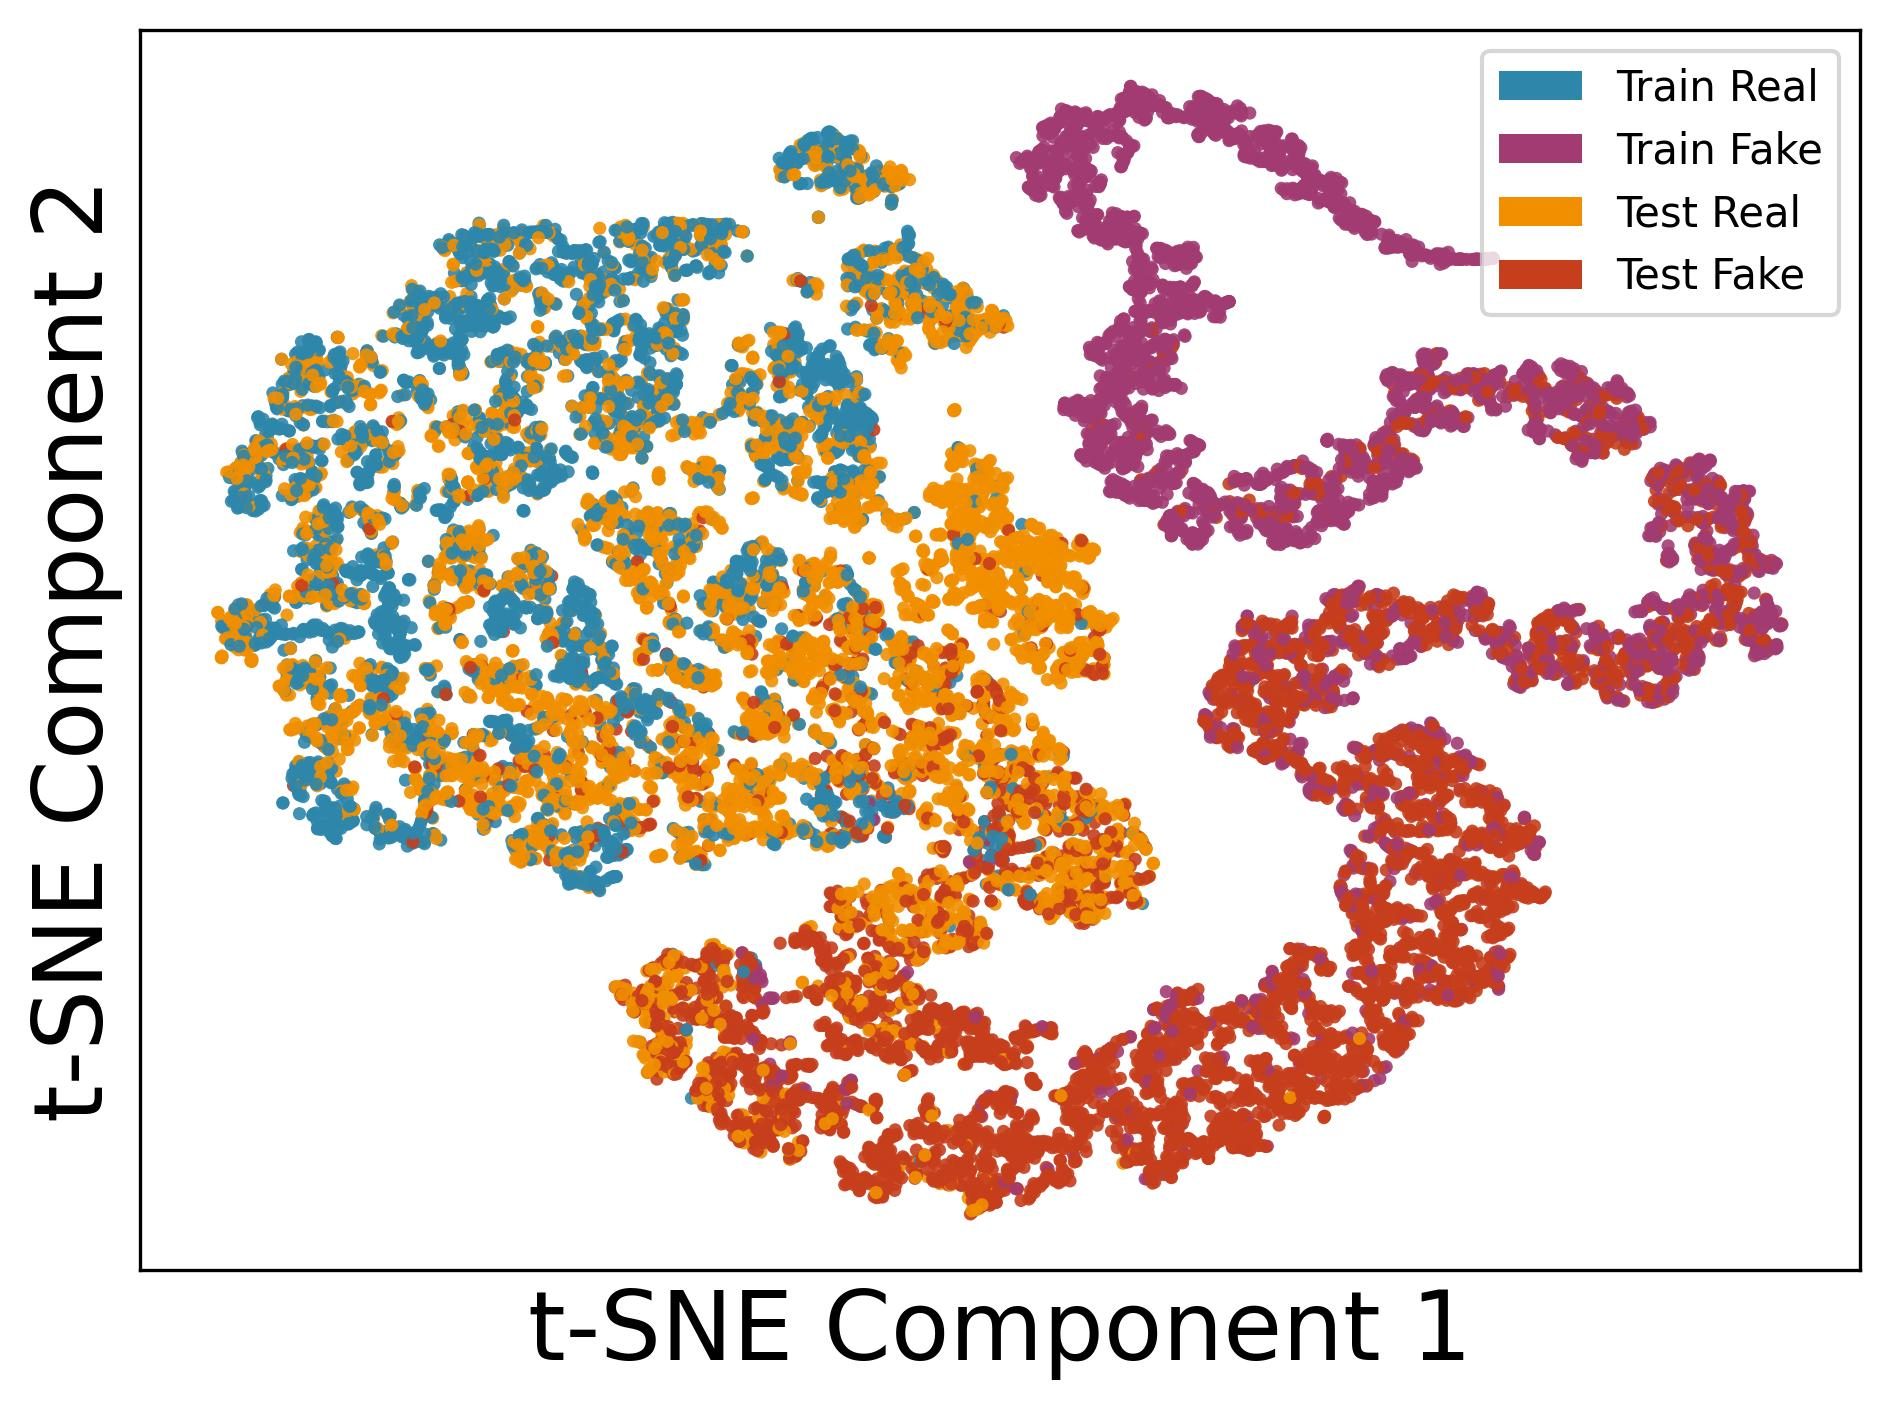
\includegraphics[width=\linewidth]{proposal/images/simlbr/tsne_w_lbr_wukong.jpeg}\\
  {\small (b) w/ LBR}
\end{minipage}
\caption{\textbf{t-SNE visualization of Latent Blending Regularization:} Detectors trained without LBR overfit to generator-specific artifacts, so fake images from an unseen generator (Wukong, red points) are misclassified as real. With LBR, the detector learns a tight boundary around the real image distribution (blue/orange cluster), and any sample outside this region, regardless of its generative source, is classified as fake. The detector is trained on ProGAN images.}
\label{fig:simlbr_tsne}
\end{figure}

\subsubsection{Fake Image Detection as Learning a Tight Boundary Around Real Images}
Ojha et al.~\cite{ojha2023towards} showed that, during training, most detectors learn to identify generator-specific fingerprints rather than the underlying distributional differences between real and fake images. When these fingerprints are absent from a new generator, the detector classifies its fakes as real, effectively treating the real category as a \textit{sink class}: a class that absorbs all out-of-distribution samples regardless of their true label. This behavior was further highlighted by AIDE~\cite{yansanity}, which argued that common benchmarks such as AIGC~\cite{wang2020cnn} and GenImage~\cite{zhu2023genimage} contain randomly generated images with no guarantee of perceptual quality, and introduced Chameleon, a test set of fake images that pass a human perception \textit{Turing Test}. State-of-the-art detectors, including UnivFD~\cite{ojha2023towards} and AIDE~\cite{yansanity}, degrade severely on Chameleon, and the degradation is caused primarily by fake images being classified as real.

Learning a tight boundary around the fake samples seen during training is highly undesirable, because the distribution of fake images is continually evolving. New generative models with completely different structures and artifacts are constantly introduced, pushing their samples outside the learned boundary. In contrast, the distribution of real images remains relatively stable. Shifts caused by improved camera sensors are minor and occur over long periods of time. We therefore propose that fake image detection should be solved by learning a tight boundary around the \textit{real} image distribution and using the fake category as the sink class. Intuitively, anything that is not real can be placed in the fake category, irrespective of the nature and origin of the fake sample.

One way to model only the real distribution is to frame the problem as anomaly detection~\cite{scholkopf2001ocsvm,ruff2018deep,hendrycks2017baseline}. However, in the extremely high-dimensional space of natural images, the assumption that photorealistic fakes will naturally fall outside the learned real-image manifold is unrealistic. We verify this in Section~\ref{sec:simlbr_ablation}, where a One-Class SVM trained on the same features substantially underperforms SimLBR. Effective discrimination therefore requires training signals derived from fake images that guide the model toward a meaningful boundary. Several face-forgery detectors~\cite{nguyen2024laa,Shiohara_2022_CVPR,tian2024real} construct pseudo-fakes by applying hand-crafted manipulations to real images. However, these methods operate in pixel space, often require task-specific preprocessing such as facial landmark detection, and introduce only a narrow family of low-level artifacts. SimLBR instead constructs pseudo-fakes in the latent space of a pretrained foundation model, using guidance from real fake images.

\subsubsection{Measuring Reliability and Worst-Case Performance}
\label{sec:reliability}
Most fake image detection works report average accuracy across generators as the key measure of performance. However, detectors often exhibit high variance across generators: a model may achieve over 99\% accuracy on one generator and drop to nearly 50\% on another. The true utility of a detector lies in its robustness to the next generation of models that are unknown at training time, so the variance across generators is a critical dimension of evaluation. To quantify the trade-off between accuracy and stability, we adapt the Sharpe ratio~\cite{sharpe1994ratio}, which measures excess return relative to risk, and define the \textit{Reliability} of a detector as:
\begin{equation}
\text{Reliability} = \frac{\mu_{\text{acc}} - A_{\text{base}}}{\sigma_{\text{acc}}}
\label{eq:reliability}
\end{equation}
where $\mu_{\text{acc}}$ is the mean accuracy across all evaluated generators, $\sigma_{\text{acc}}$ is the corresponding standard deviation, and $A_{\text{base}}$ is the accuracy of a naive ``risk-free'' baseline. We set $A_{\text{base}}=50$, the accuracy of a random predictor. A higher reliability indicates a detector that is both accurate and stable across generators.

We additionally report a \textit{Worst-Case Estimate} (WCE), defined as the lowest accuracy of a detector across all evaluated generators. This quantity approximates the performance of the detector when confronted with a future generator that deviates most from the training distribution, and serves as an upper bound on its true worst-case performance in the open world.

\begin{figure}[!t]
\begin{center}
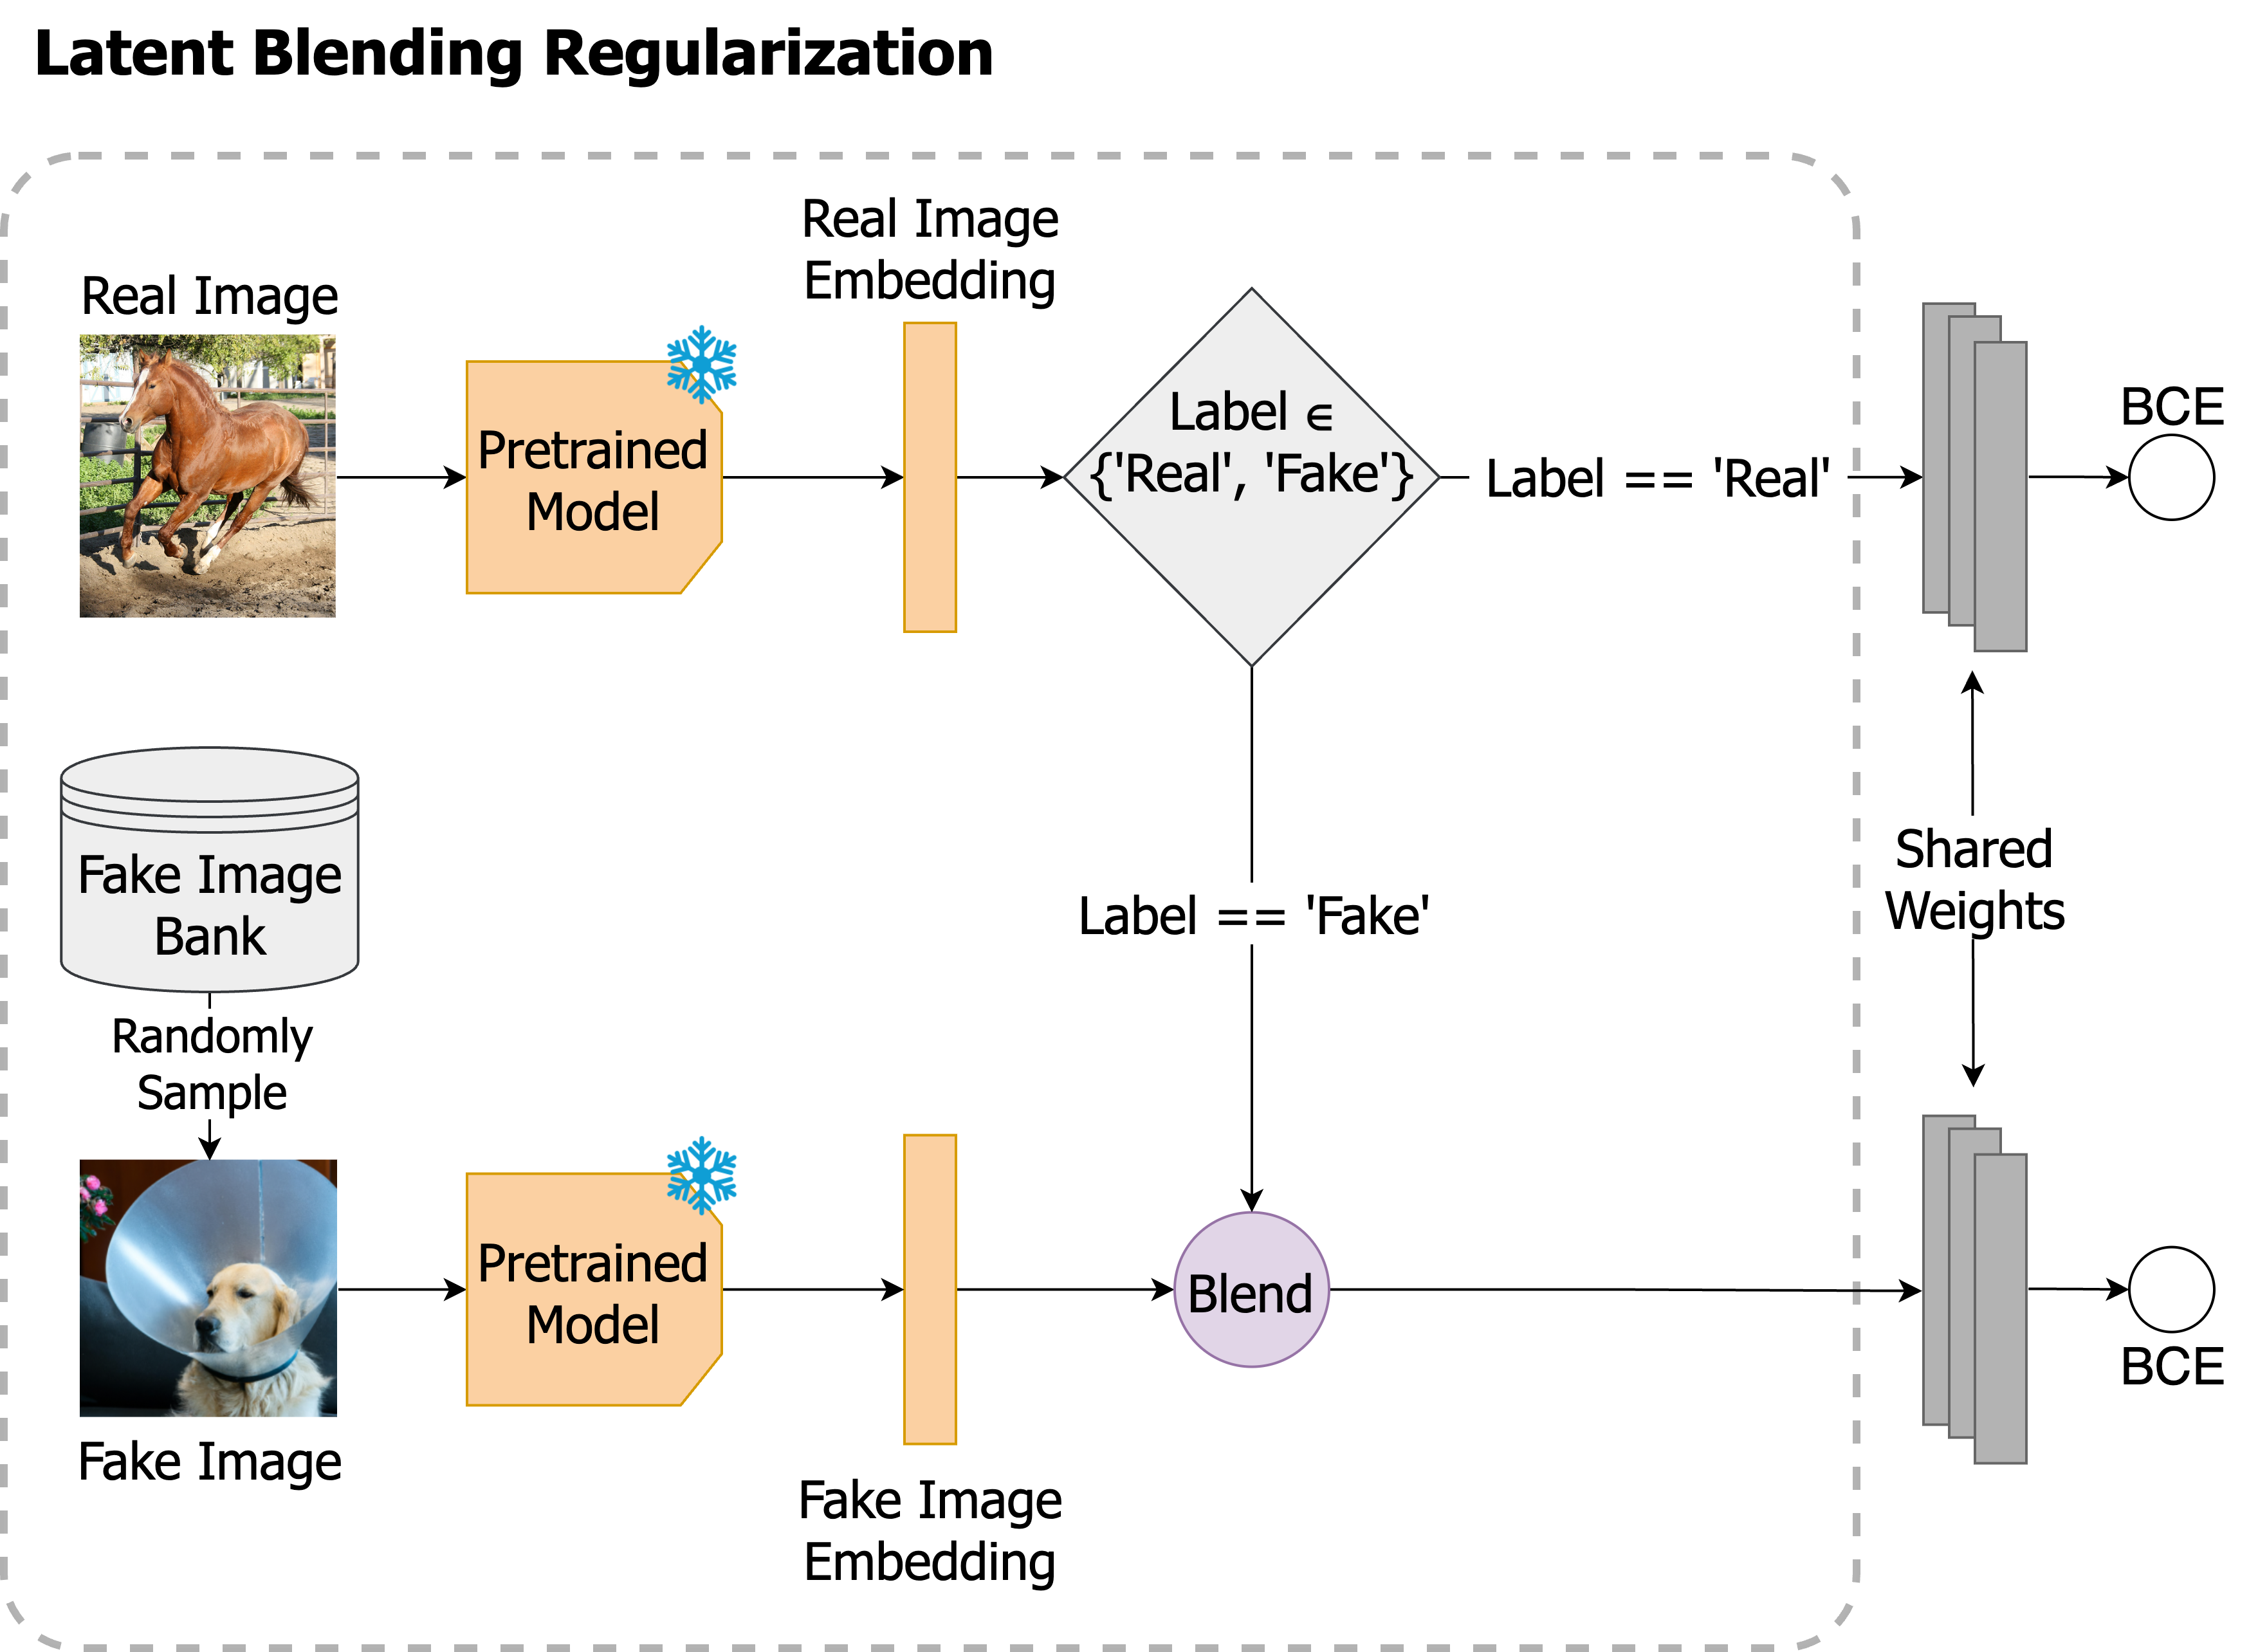
\includegraphics[width=\linewidth]{proposal/images/simlbr/simlbr_framework.png}
\end{center}
\caption{\textbf{Framework of SimLBR:} For each real image in the training set, the model samples either a real or a fake label. If a fake label is sampled, a small amount of fake image information is blended into the real image representation in a pretrained latent space. Solving this objective forces the model to learn a tight decision boundary around the unperturbed real image distribution, enabling better generalization to unseen generative models.}
\label{fig:simlbr_framework}
\end{figure}

\begin{figure}[!t]
\begin{center}
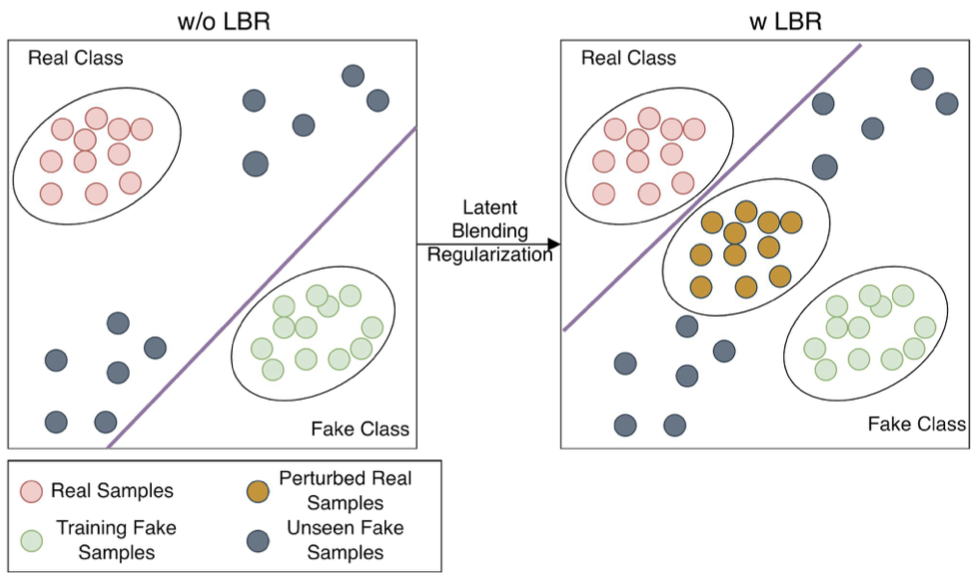
\includegraphics[width=0.85\linewidth]{proposal/images/simlbr/lbr_boundary_schematic.png}
\end{center}
\caption{\textbf{Intuition behind Latent Blending Regularization:} Without LBR (left), the detector learns a boundary that tightly encloses the training fakes, so unseen fakes fall on the real side of the boundary. LBR introduces perturbed real samples (yellow) that lie just outside the real distribution and are labeled as fake. This pushes the decision boundary toward the real distribution (right), so that unseen fakes from any generator are classified as fake.}
\label{fig:lbr_schematic}
\end{figure}

\subsubsection{Method}
Following prior work, we train on fake images from a single source generator $G_s$ and evaluate on a set of unseen generators $\mathbb{U}=\{U_1, U_2, \ldots, U_m\}$. Let $\mathbb{R}=\{R_1, R_2, \ldots, R_n\}$ be the set of real training images, $\mathbb{F}=\{F_1, F_2, \ldots, F_n\}$ the set of fake training images, and $I$ a frozen, pretrained image feature extractor. During training, a real image $R_i$ is sampled and assigned a random label $y_i \in \{0,1\}$. If $y_i=0$, its features are computed as $L_i = I(R_i)$. If $y_i=1$, we compute its features using Latent Blending Regularization.

\noindent\textbf{Latent Blending Regularization (LBR):} For a real image $R_i$ with label $y_i=1$, we randomly sample a fake image $F_i$ from the training set and compute the features of both images:
\begin{equation}
L_i^{R} = I(R_i), \qquad L_i^{F} = I(F_i)
\label{eq:lbr_features}
\end{equation}
The final representation is a linear interpolation between the two latent representations:
\begin{equation}
L_i = \alpha L_i^{R} + (1-\alpha) L_i^{F}
\label{eq:lbr}
\end{equation}
The overall training setup is summarized in Figure~\ref{fig:simlbr_framework}, and the intended effect on the decision boundary is illustrated in Figure~\ref{fig:lbr_schematic}. The key idea is that even a small injection of fake information into a real image should be classified as fake. This forces the detector to recognize only completely unaltered, truly authentic images as real, thereby compelling it to model the structure of the real distribution.

Blending in the latent space of a pretrained model, rather than in pixel space~\cite{zhang2018mixup}, is central to our approach and differs from prior blending strategies in both motivation and formulation~\cite{Shiohara_2022_CVPR,verma2019manifold}. First, perturbed samples are constructed efficiently through simple vector arithmetic. Second, $\alpha$ gives fine-grained control over the amount of fake information that is injected, enabling a virtually unlimited number of perturbed real samples. Most importantly, blending in a semantic latent space keeps the classification of real images non-trivial. When blending occurs in pixel space, low-level artifacts can be copied directly from the fake image, and the model can identify perturbed samples by detecting these artifacts. Latent-space blending operates on higher-level representations where such low-level cues are less likely to be preserved, forcing the detector to learn meaningful distinctions and enforce a tighter boundary around the real distribution. We use DINOv3~\cite{simeoni2025dinov3}, whose expressive representations preserve high-level structure and semantics, enabling meaningful interpolation between real and fake samples.

\noindent\textbf{Sampling distribution for $\alpha$:} The choice of sampling distribution for $\alpha$ directly determines how effectively the regularizer makes real-image classification non-trivial. Low values of $\alpha$ inject a large proportion of fake information, producing representations that are trivially identified as fake. Conversely, extremely high values of $\alpha$ (e.g., $\alpha=0.99$) produce blended representations that are almost indistinguishable from real samples, forcing the model to separate nearly identical embeddings into different classes, which is an unstable training scenario. We adopt the intuition that a meaningful perturbed real sample should retain the majority of the information from the real image while incorporating only a small proportion from the fake image. Accordingly, we sample:
\begin{equation}
\alpha \sim \text{Uniform}(0.5, B)
\label{eq:alpha_sampling}
\end{equation}
where $B$ is an upper bound. We verify this choice with an ablation study in Section~\ref{sec:simlbr_ablation}.

\noindent\textbf{Training objective:} The features are passed through a lightweight MLP $F_\theta$, which is trained with the Binary Cross-Entropy (BCE) objective:
\begin{equation}
\mathcal{L}_{\text{BCE}} = -\frac{1}{N} \sum_{i=1}^{N} \left[ y_i \log F_{\theta}(L_i) + (1 - y_i) \log\left(1 - F_{\theta}(L_i)\right) \right]
\label{eq:simlbr_bce}
\end{equation}
For implementation simplicity, instead of resampling labels for the same real image, we iterate over the entire training set and, whenever a fake image is encountered, sample a real image to form a pair and assign the blended representation a fake label. This pairing ensures that all real and fake training samples are used.

\subsubsection{Experimental Setup}
\noindent\textbf{Implementation details:} We use DINOv3~\cite{simeoni2025dinov3} as the feature extractor in all experiments. For efficiency, we precompute embeddings for the entire training set and train a two-layer MLP classifier with ReLU activations on these features. SimLBR is trained with a batch size of 500 for a maximum of 10 epochs, with the upper bound $B$ of the $\alpha$ distribution set to $0.8$. We use the Adam optimizer with a learning rate of \texttt{1e-4} and weight decay of \texttt{1e-2}. After embeddings are precomputed, a training run requires approximately 3 minutes on a single NVIDIA H100 GPU. Precomputing the embeddings takes around 50 minutes for the AIGC and 22 minutes for the GenImage training sets. For comparison, the previous state-of-the-art method, AIDE~\cite{yansanity}, was trained on eight NVIDIA A100 GPUs for roughly two hours.

\noindent\textbf{Datasets:} We follow the standard cross-generator protocol: the detector is trained on fake images from a single generator and evaluated on images from a set of unseen generators. We evaluate on four benchmarks:
\begin{itemize}
    \item \textbf{GenImage}~\cite{zhu2023genimage}: we train on Stable Diffusion v1.4~\cite{rombach2022high} and evaluate on 7 other generators.
    \item \textbf{AIGC}~\cite{wang2020cnn}: we train on ProGAN~\cite{karras2017progressive} and evaluate on 15 other generators.
    \item \textbf{Chameleon}~\cite{yansanity}: a curated hard test set of fake images that pass a human perception test. We evaluate models trained on ProGAN and on Stable Diffusion v1.4.
    \item \textbf{RSFake-1M}~\cite{tan2025rsfake}: 500,000 real and 500,000 synthetic satellite images from 10 satellite-specific diffusion models (DiffusionSat-512, DiffusionSat-256~\cite{khanna2024diffusionsat}, GeoRSSD, SDFRS, GeoSynth-Text, GeoSynth-SAM, GeoSynth-Canny, CRSDiff, MapSat, and RSPaint). We train on DiffusionSat-512 and DiffusionSat-256 and evaluate on held-out test sets from all ten models. For this benchmark, we use the DINOv3-Satellite backbone, which is pretrained on 493M satellite images.
\end{itemize}
Along with average accuracy, we report the standard deviation across generators, the reliability score (Equation~\ref{eq:reliability}), and the worst-case estimate.

\begin{table*}[!t]
\resizebox{\linewidth}{!}{
\begin{tabular}{l|c|ccccccc|ccc}
Method & \begin{tabular}[c]{@{}c@{}}SD v1.4\\ (Training)\end{tabular} & Midjourney & SD v1.5 & ADM & GLIDE & Wukong & VQDM & BigGAN & \textit{Mean}$\uparrow$ & \textit{Std}$\downarrow$ & \textit{Rel.}$\uparrow$ \\
\hline
ResNet-50  & \textbf{99.90} & 54.90 & 99.70 & 53.50 & 61.90 & 98.20 & 56.60 & 52.00 & 72.09 & 22.70 & 0.97 \\
DeiT-S     & \textbf{99.90} & 55.60 & 99.80 & 49.80 & 58.10 & 98.90 & 56.90 & 53.50 & 71.56 & 23.29 & 0.92 \\
Swin-T     & \textbf{99.90} & 62.10 & 99.80 & 49.80 & 67.60 & 99.10 & 62.30 & 57.60 & 74.78 & 21.17 & 1.17 \\
CNNSpot    & 96.30 & 52.80 & 95.90 & 50.10 & 39.80 & 78.60 & 53.40 & 46.80 & 64.21 & 22.63 & 0.62 \\
Spec       & 99.40 & 52.00 & 99.20 & 49.70 & 49.80 & 94.80 & 55.60 & 49.80 & 68.79 & 24.14 & 0.77 \\
F3Net      & \textbf{99.90} & 50.10 & \underline{99.90} & 49.90 & 50.00 & \textbf{99.90} & 49.90 & 49.90 & 68.69 & 25.85 & 0.72 \\
GramNet    & 99.20 & 54.20 & 99.10 & 50.30 & 54.60 & 98.80 & 50.80 & 51.70 & 68.85 & 24.22 & 0.77 \\
DIRE       & \textbf{99.90} & 60.20 & 99.80 & 50.90 & 55.00 & \underline{99.20} & 50.10 & 50.20 & 70.66 & 24.22 & 0.85 \\
UnivFD     & 84.20 & 73.20 & 84.00 & 55.20 & 76.90 & 75.60 & 56.90 & \underline{80.30} & 73.29 & 11.32 & 2.05 \\
GenDet     & 96.10 & \underline{89.60} & 96.10 & 58.00 & 78.40 & 92.80 & 66.50 & 75.00 & 81.56 & 14.39 & 2.19 \\
PatchCraft & 89.50 & 79.00 & 89.30 & 77.30 & 78.40 & 89.30 & \underline{83.70} & 72.40 & 82.30 & \underline{6.56} & \underline{4.29} \\
AIDE       & \underline{99.74} & 79.38 & 99.76 & \underline{78.54} & \underline{91.82} & 98.65 & 80.26 & 66.89 & \underline{86.88} & 12.33 & 2.99 \\
\hline
SimLBR     & 98.28 & \textbf{91.67} & 98.10 & \textbf{96.98} & \textbf{92.38} & 97.44 & \textbf{93.50} & \textbf{88.00} & \textbf{94.54} & \textbf{3.74} & \textbf{11.91}
\end{tabular}
}
\caption{\textbf{Evaluation on GenImage:} All models are trained on Stable Diffusion v1.4 and evaluated on the other generators. SimLBR outperforms the state of the art on 5 of the 7 unseen generators, with the largest gain on BigGAN, a GAN-based generator with very different artifacts from the diffusion-based training generator. SimLBR also has the lowest standard deviation and the highest reliability.}
\label{table:simlbr_genimage}
\end{table*}

\begin{table*}[!t]
\resizebox{\linewidth}{!}{
\begin{tabular}{l|ccccccccccc|c}
Method & CNNSpot & FreDect & Fusing & LNP & LGrad & UnivFD & DIRE-G & DIRE-D & PatchCraft & NPR & AIDE & SimLBR \\
\hline
ProGAN (Training) & \textbf{100.0} & 99.36 & \textbf{100.0} & 99.67 & 99.83 & 99.81 & 95.19 & 52.75 & \textbf{100.0} & 99.79 & \underline{99.99} & 99.29 \\
\hline
StyleGAN   & 90.17 & 78.02 & 85.2 & 91.75 & 91.08 & 84.93 & 83.03 & 51.31 & 92.77 & \underline{97.70} & \textbf{99.64} & 87.38 \\
BigGAN     & 71.17 & 81.97 & 77.4 & 77.75 & 85.62 & 95.08 & 70.12 & 49.7 & \underline{95.80} & 84.35 & 83.95 & \textbf{95.52} \\
CycleGAN   & 87.62 & 78.77 & 87.0 & 84.1 & 86.94 & \underline{98.33} & 74.19 & 49.58 & 70.17 & 96.1 & \textbf{98.48} & 88.11 \\
StarGAN    & 94.6 & 94.62 & 97.0 & \underline{99.92} & 99.27 & 95.75 & 95.47 & 46.72 & \textbf{99.97} & 99.35 & 99.91 & 88.54 \\
GauGAN     & 81.42 & 80.57 & 77.0 & 75.39 & 78.46 & \textbf{99.47} & 67.79 & 51.23 & 71.58 & 82.5 & 73.25 & \underline{97.14} \\
StyleGAN2  & 86.91 & 66.19 & 83.3 & 94.64 & 85.32 & 74.96 & 75.31 & 51.72 & 89.55 & \textbf{98.38} & \underline{98.00} & 84.57 \\
WFIR       & \underline{91.65} & 50.75 & 66.8 & 70.85 & 55.7 & 86.9 & 58.05 & 53.3 & 85.8 & 65.8 & \textbf{94.2} & 89.50 \\
ADM        & 60.39 & 63.42 & 49.0 & 84.73 & 67.15 & 66.87 & 75.78 & \textbf{98.25} & 82.17 & 69.69 & \underline{93.43} & 85.89 \\
Glide      & 58.07 & 54.13 & 57.2 & 80.52 & 66.11 & 62.46 & 71.75 & \underline{92.42} & 83.79 & 78.36 & \textbf{95.09} & 90.88 \\
Midjourney & 51.39 & 45.87 & 52.2 & 65.55 & 65.35 & 56.13 & 58.01 & \underline{89.45} & \textbf{90.12} & 77.85 & 77.2 & 75.54 \\
SD v1.4    & 50.57 & 38.79 & 51.0 & 85.55 & 63.02 & 63.66 & 49.74 & 91.24 & \textbf{95.38} & 78.63 & \underline{93.00} & 85.51 \\
SD v1.5    & 50.53 & 39.21 & 51.4 & 85.67 & 63.67 & 63.49 & 49.83 & 91.63 & \textbf{95.30} & 78.89 & \underline{92.85} & 84.43 \\
VQDM       & 56.46 & 77.8 & 55.1 & 74.46 & 72.99 & 85.31 & 53.68 & 91.9 & 88.91 & 78.13 & \textbf{95.16} & \underline{93.20} \\
Wukong     & 51.03 & 40.3 & 51.7 & 82.06 & 59.55 & 70.93 & 54.46 & 90.9 & \underline{91.07} & 76.11 & \textbf{93.55} & 90.08 \\
DALLE2     & 50.45 & 34.7 & 52.8 & 88.75 & 65.45 & 50.75 & 66.48 & 92.45 & \underline{96.60} & 64.90 & \textbf{96.60} & 78.80 \\
\hline
\textit{Mean}$\uparrow$        & 70.78 & 64.03 & 68.38 & 83.84 & 75.34 & 78.43 & 68.68 & 71.53 & \underline{89.31} & 82.91 & \textbf{92.77} & 88.40 \\
\textit{Std}$\downarrow$         & 18.91 & 21.08 & 18.04 & 9.78 & 14.26 & 16.73 & 14.46 & 21.55 & 8.89 & 11.92 & \underline{7.92} & \textbf{6.23} \\
\textit{Reliability}$\uparrow$ & 1.10 & 0.67 & 1.02 & 3.46 & 1.78 & 1.70 & 1.29 & 1.00 & 4.42 & 2.76 & \underline{5.40} & \textbf{6.16}
\end{tabular}
}
\caption{\textbf{Evaluation on AIGC:} All models are trained on ProGAN and evaluated on 15 other generators. SimLBR has the third-highest average accuracy, and it is the most consistent detector, with the lowest standard deviation and the highest reliability. SimLBR is also the only detector that achieves above 75\% accuracy on every generator.}
\label{table:simlbr_aigc}
\end{table*}

\begin{table*}[!t]
\resizebox{\linewidth}{!}{
\begin{tabular}{c|cccccccccc|c}
\hline
\textbf{Training Set} & \textbf{CNNSpot} & \textbf{FreDect} & \textbf{Fusing} & \textbf{GramNet} & \textbf{LNP} & \textbf{UnivFD} & \textbf{DIRE} & \textbf{PatchCraft} & \textbf{NPR} & \textbf{AIDE} & \textbf{SimLBR} \\
\hline
\multirow{2}{*}{\textbf{ProGAN}} & 56.94 & 55.62 & 56.98 & 58.94 & 57.11 & 57.22 & 58.19 & 53.76 & 57.29 & 58.37 & \textbf{84.33} \\
 & 0.08/99.67 & 13.72/87.12 & 0.01/99.79 & 4.76/99.66 & 0.09/99.97 & 3.18/97.83 & 3.25/99.48 & 1.78/92.82 & 2.20/98.70 & 5.04/98.46 & \textbf{75.80}/90.74 \\
\cline{2-12}
\multirow{2}{*}{\textbf{SD v1.4}} & 60.11 & 56.86 & 57.07 & 60.95 & 55.63 & 55.62 & 59.71 & 56.32 & 58.13 & 62.60 & \textbf{85.57} \\
 & 8.86/98.63 & 1.37/98.57 & 0.00/99.96 & 17.65/93.50 & 0.57/97.01 & 74.97/41.09 & 11.86/95.67 & 3.07/96.35 & 2.43/100.00 & 20.33/94.38 & \textbf{92.96}/80.06 \\
\hline
\end{tabular}
}
\caption{\textbf{Evaluation on the hard test set Chameleon:} For each training setting, the first row reports overall accuracy and the second row reports fake/real accuracy. Results for prior methods are taken from AIDE~\cite{yansanity}. All existing detectors deteriorate severely and classify almost all fake images as real. SimLBR maintains its performance, showing strong robustness to shifts in the generator distribution.}
\label{table:simlbr_chameleon}
\end{table*}

\begin{table}[!t]
\centering
\begin{tabular}{l|ccccc|c}
\hline
 & CNNSpot & UnivFD & DIRE & PatchCraft & AIDE & SimLBR \\
\hline
GenImage & 50.10 & 55.20 & 50.10 & \underline{72.40} & 66.89 & \textbf{88.00} \\
AIGC     & 50.45 & 50.75 & 49.74 & 70.17 & \underline{73.25} & \textbf{75.54} \\
\hline
\end{tabular}
\caption{\textbf{Worst-case estimates:} The lowest accuracy of each detector across all test generators. SimLBR has the best worst-case estimate on both AIGC and GenImage, suggesting it is more dependable when deployed in real-world settings.}
\label{table:simlbr_worst}
\end{table}

\subsubsection{Results}
\noindent\textbf{GenImage:} Table~\ref{table:simlbr_genimage} shows the results on GenImage. SimLBR achieves the highest average accuracy of $94.54\%$, outperforming the previous state of the art by $7.66\%$. One of the largest gains is on BigGAN~\cite{brock2018large}, a GAN-based model whose artifacts differ greatly from those of the diffusion-based training generator. This suggests that SimLBR models the real distribution and is much less affected by changes in the distribution of fake images. SimLBR also has the lowest standard deviation ($3.74$) and the highest reliability ($11.91$, compared to $4.29$ for the next best method).

\noindent\textbf{AIGC:} Table~\ref{table:simlbr_aigc} shows that SimLBR remains competitive with state-of-the-art approaches on AIGC, achieving the third-highest average accuracy. More importantly, it is the most consistent detector across generators, with the lowest standard deviation and the highest reliability. Notably, SimLBR is the only model that achieves above $75\%$ accuracy on every generator.

\noindent\textbf{Chameleon:} Table~\ref{table:simlbr_chameleon} presents the results on the curated hard test set Chameleon. Unlike existing methods, SimLBR does not degrade on this test set. It surpasses prior state-of-the-art models by up to $24.85\%$ in accuracy and up to $69.62\%$ in recall. These gains show that SimLBR avoids the common failure mode of detectors that overfit to specific generators and collapse on new synthesis techniques. Most existing detectors classify nearly all Chameleon fakes as real, which is exactly the behavior expected when the real category acts as a sink class.

\noindent\textbf{Worst-case performance:} Table~\ref{table:simlbr_worst} reports the worst-case estimates of state-of-the-art detectors on GenImage and AIGC. SimLBR achieves the highest worst-case estimate in both settings ($88.00\%$ and $75.54\%$), indicating that it maintains strong performance even under large distribution shifts and is well suited to deployment alongside continually evolving generative models.

\noindent\textbf{Robustness to image perturbations:} Prior works~\cite{yansanity,zhong2023patchcraft} show that detectors degrade severely when perturbations such as JPEG compression and Gaussian blur are applied to the input. Table~\ref{table:simlbr_perturb} reports the average accuracy across the 16 AIGC generators under different perturbations. SimLBR achieves the highest accuracy under every perturbation, even though, unlike most prior methods~\cite{yansanity,zhong2023patchcraft,wang2020cnn}, we did not use JPEG compression or Gaussian blur augmentation during training.

\begin{table*}[!t]
\resizebox{\linewidth}{!}{
\begin{tabular}{lc|cccc|cccc}
\hline
\multirow{2}{*}{\textbf{Method}} & \multirow{2}{*}{\textbf{Original}} & \multicolumn{4}{c|}{\textbf{JPEG Compression}} & \multicolumn{4}{c}{\textbf{Gaussian Blur}} \\
 & & \textbf{QF=95} & \textbf{QF=90} & \textbf{QF=75} & \textbf{QF=50} & $\sigma=1.0$ & $\sigma=2.0$ & $\sigma=3.0$ & $\sigma=4.0$ \\
\hline
CNNSpot    & 70.78 & 64.03 & 62.26 & 60.65 & 59.66 & 68.39 & 67.26 & 67.13 & 65.85 \\
FreDect    & 64.03 & 66.95 & 67.45 & 66.64 & 65.33 & 65.75 & 66.48 & 68.58 & 69.64 \\
Fusing     & 68.38 & 62.43 & 61.39 & 59.34 & 57.41 & 68.09 & 66.69 & 66.02 & 65.58 \\
LNP        & 83.84 & 53.58 & 54.09 & 53.02 & 52.85 & 67.91 & 66.42 & 66.2 & 62.69 \\
LGrad      & 75.34 & 51.55 & 51.39 & 50.00 & 50.00 & 71.73 & 69.12 & 68.43 & 66.22 \\
DIRE-G     & 68.68 & 66.49 & 66.12 & 65.28 & 64.34 & 64.00 & 63.09 & 62.21 & 61.91 \\
UnivFD     & 78.43 & 74.10 & 74.02 & 69.92 & 68.68 & 70.31 & 68.29 & 64.62 & 61.18 \\
PatchCraft & 89.31 & 72.48 & 71.41 & 69.43 & 67.78 & 75.99 & 74.90 & 73.53 & 72.28 \\
AIDE       & \textbf{92.77} & 75.54 & 74.21 & 70.64 & 69.60 & 81.88 & 80.35 & 80.05 & 79.86 \\
\hline
SimLBR     & 88.40 & \textbf{86.04} & \textbf{83.92} & \textbf{78.98} & \textbf{73.48} & \textbf{88.03} & \textbf{86.65} & \textbf{86.39} & \textbf{86.30} \\
\hline
\end{tabular}
}
\caption{\textbf{Robustness to JPEG compression and Gaussian blur:} Average accuracy across the AIGC generators when different amounts of JPEG compression and Gaussian blur are applied to the input images. SimLBR shows minimal degradation, even under strong perturbations that it never saw during training.}
\label{table:simlbr_perturb}
\end{table*}

\begin{table*}[!t]
\resizebox{\linewidth}{!}{
\begin{tabular}{cc|cc|cc|c|ccccc}
\hline
 & & \multicolumn{2}{c|}{\textbf{ProGAN}} & \multicolumn{2}{c|}{\textbf{SD v1.4}} & \textbf{DiffusionSat} & & & & & \\
\multirow{-2}{*}{\textbf{Backbone}} & \multirow{-2}{*}{\textbf{LBR}} & \textbf{Chameleon} & \textbf{AIGC} & \textbf{Chameleon} & \textbf{GenImage} & \textbf{RSFake} & \multirow{-2}{*}{\textbf{Mean Acc.}$\uparrow$} & \multirow{-2}{*}{\textbf{Mean Rec.}$\uparrow$} & \multirow{-2}{*}{\textbf{Std}$\downarrow$} & \multirow{-2}{*}{\textbf{Reliability}$\uparrow$} & \multirow{-2}{*}{\textbf{WCE}$\uparrow$} \\
\hline
DINOv2 & \ding{55} & \begin{tabular}[c]{@{}c@{}}56.12\\ 0.64/97.83\end{tabular} & \begin{tabular}[c]{@{}c@{}}70.77\\ 44.45/97.09\end{tabular} & \begin{tabular}[c]{@{}c@{}}62.04\\ 60.73/63.78\end{tabular} & \begin{tabular}[c]{@{}c@{}}86.74\\ 77.02/95.29\end{tabular} & - & 68.92 & 45.71 & 13.31 & 1.42 & 56.12 \\
\hline
DINOv2 & \ding{51} & \begin{tabular}[c]{@{}c@{}}55.77\\ 4.13/94.58\end{tabular} & \begin{tabular}[c]{@{}c@{}}74.75\\ 57.71/91.78\end{tabular} & \begin{tabular}[c]{@{}c@{}}62.02\\ 39.23/79.14\end{tabular} & \begin{tabular}[c]{@{}c@{}}81.49\\ 70.75/90.94\end{tabular} & - & 68.51 & 42.95 & 11.71 & 1.57 & 55.77 \\
\hline
DINOv3 & \ding{55} & \begin{tabular}[c]{@{}c@{}}59.65\\ 7.24/99.03\end{tabular} & \begin{tabular}[c]{@{}c@{}}76.70\\ 54.07/99.33\end{tabular} & \begin{tabular}[c]{@{}c@{}}87.79\\ 89.03/86.86\end{tabular} & \begin{tabular}[c]{@{}c@{}}92.19\\ 85.80/97.81\end{tabular} & \begin{tabular}[c]{@{}c@{}}73.90\\ 48.28/99.52\end{tabular} & 78.05 & 58.88 & 12.77 & 2.19 & 59.65 \\
\hline
\rowcolor{gray!20}
DINOv3 & \ding{51} & \begin{tabular}[c]{@{}c@{}}84.33\\ 75.80/90.74\end{tabular} & \begin{tabular}[c]{@{}c@{}}88.40\\ 82.07/93.97\end{tabular} & \begin{tabular}[c]{@{}c@{}}85.57\\ 92.96/80.06\end{tabular} & \begin{tabular}[c]{@{}c@{}}94.54\\ 93.89/95.05\end{tabular} & \begin{tabular}[c]{@{}c@{}}88.88\\ 78.87/99.29\end{tabular} & \begin{tabular}[c]{@{}c@{}}88.26\\ (+10.21)\end{tabular} & \begin{tabular}[c]{@{}c@{}}84.72\\ (+25.84)\end{tabular} & \begin{tabular}[c]{@{}c@{}}3.94\\ (-8.83)\end{tabular} & \begin{tabular}[c]{@{}c@{}}9.70\\ (+7.51)\end{tabular} & \begin{tabular}[c]{@{}c@{}}84.33\\ (+24.68)\end{tabular} \\
\hline
\end{tabular}
}
\caption{\textbf{Ablation of SimLBR:} We ablate the effect of latent blending regularization and of the latent space used for blending. For each setting, we report overall accuracy and fake/real accuracy. LBR significantly improves accuracy and recall in the DINOv3 latent space, and yields much better reliability and worst-case estimates. The choice of latent space is important: LBR does not give the same improvement in the DINOv2 latent space.}
\label{table:simlbr_ablate}
\end{table*}

\begin{table}[!t]
\centering
\begin{tabular}{|l|cc|cc|}
\hline
 & \multicolumn{2}{c|}{\textbf{GenImage}} & \multicolumn{2}{c|}{\textbf{AIGC}} \\
\cline{2-5}
 & ID & OD & ID & OD \\
\hline
w/o LBR & 94.37 & 77.70 & 85.58 & 73.26 \\
w/ LBR  & 95.47 & 88.00 & 91.50 & 85.98 \\
\hline
Gain & 1.10 & \textbf{10.30} & 5.92 & \textbf{12.72} \\
\hline
\end{tabular}
\caption{\textbf{Average accuracy on in-distribution (ID) and out-of-distribution (OD) generators:} ID generators share their architectural family with the training generator, while OD generators have substantially different architectures. LBR gives the largest gains on OD generators, indicating that it encourages a generator-agnostic decision boundary.}
\label{table:simlbr_idod}
\end{table}

\begin{figure}[!t]
\centering
\begin{minipage}[t]{0.48\linewidth}
  \centering
  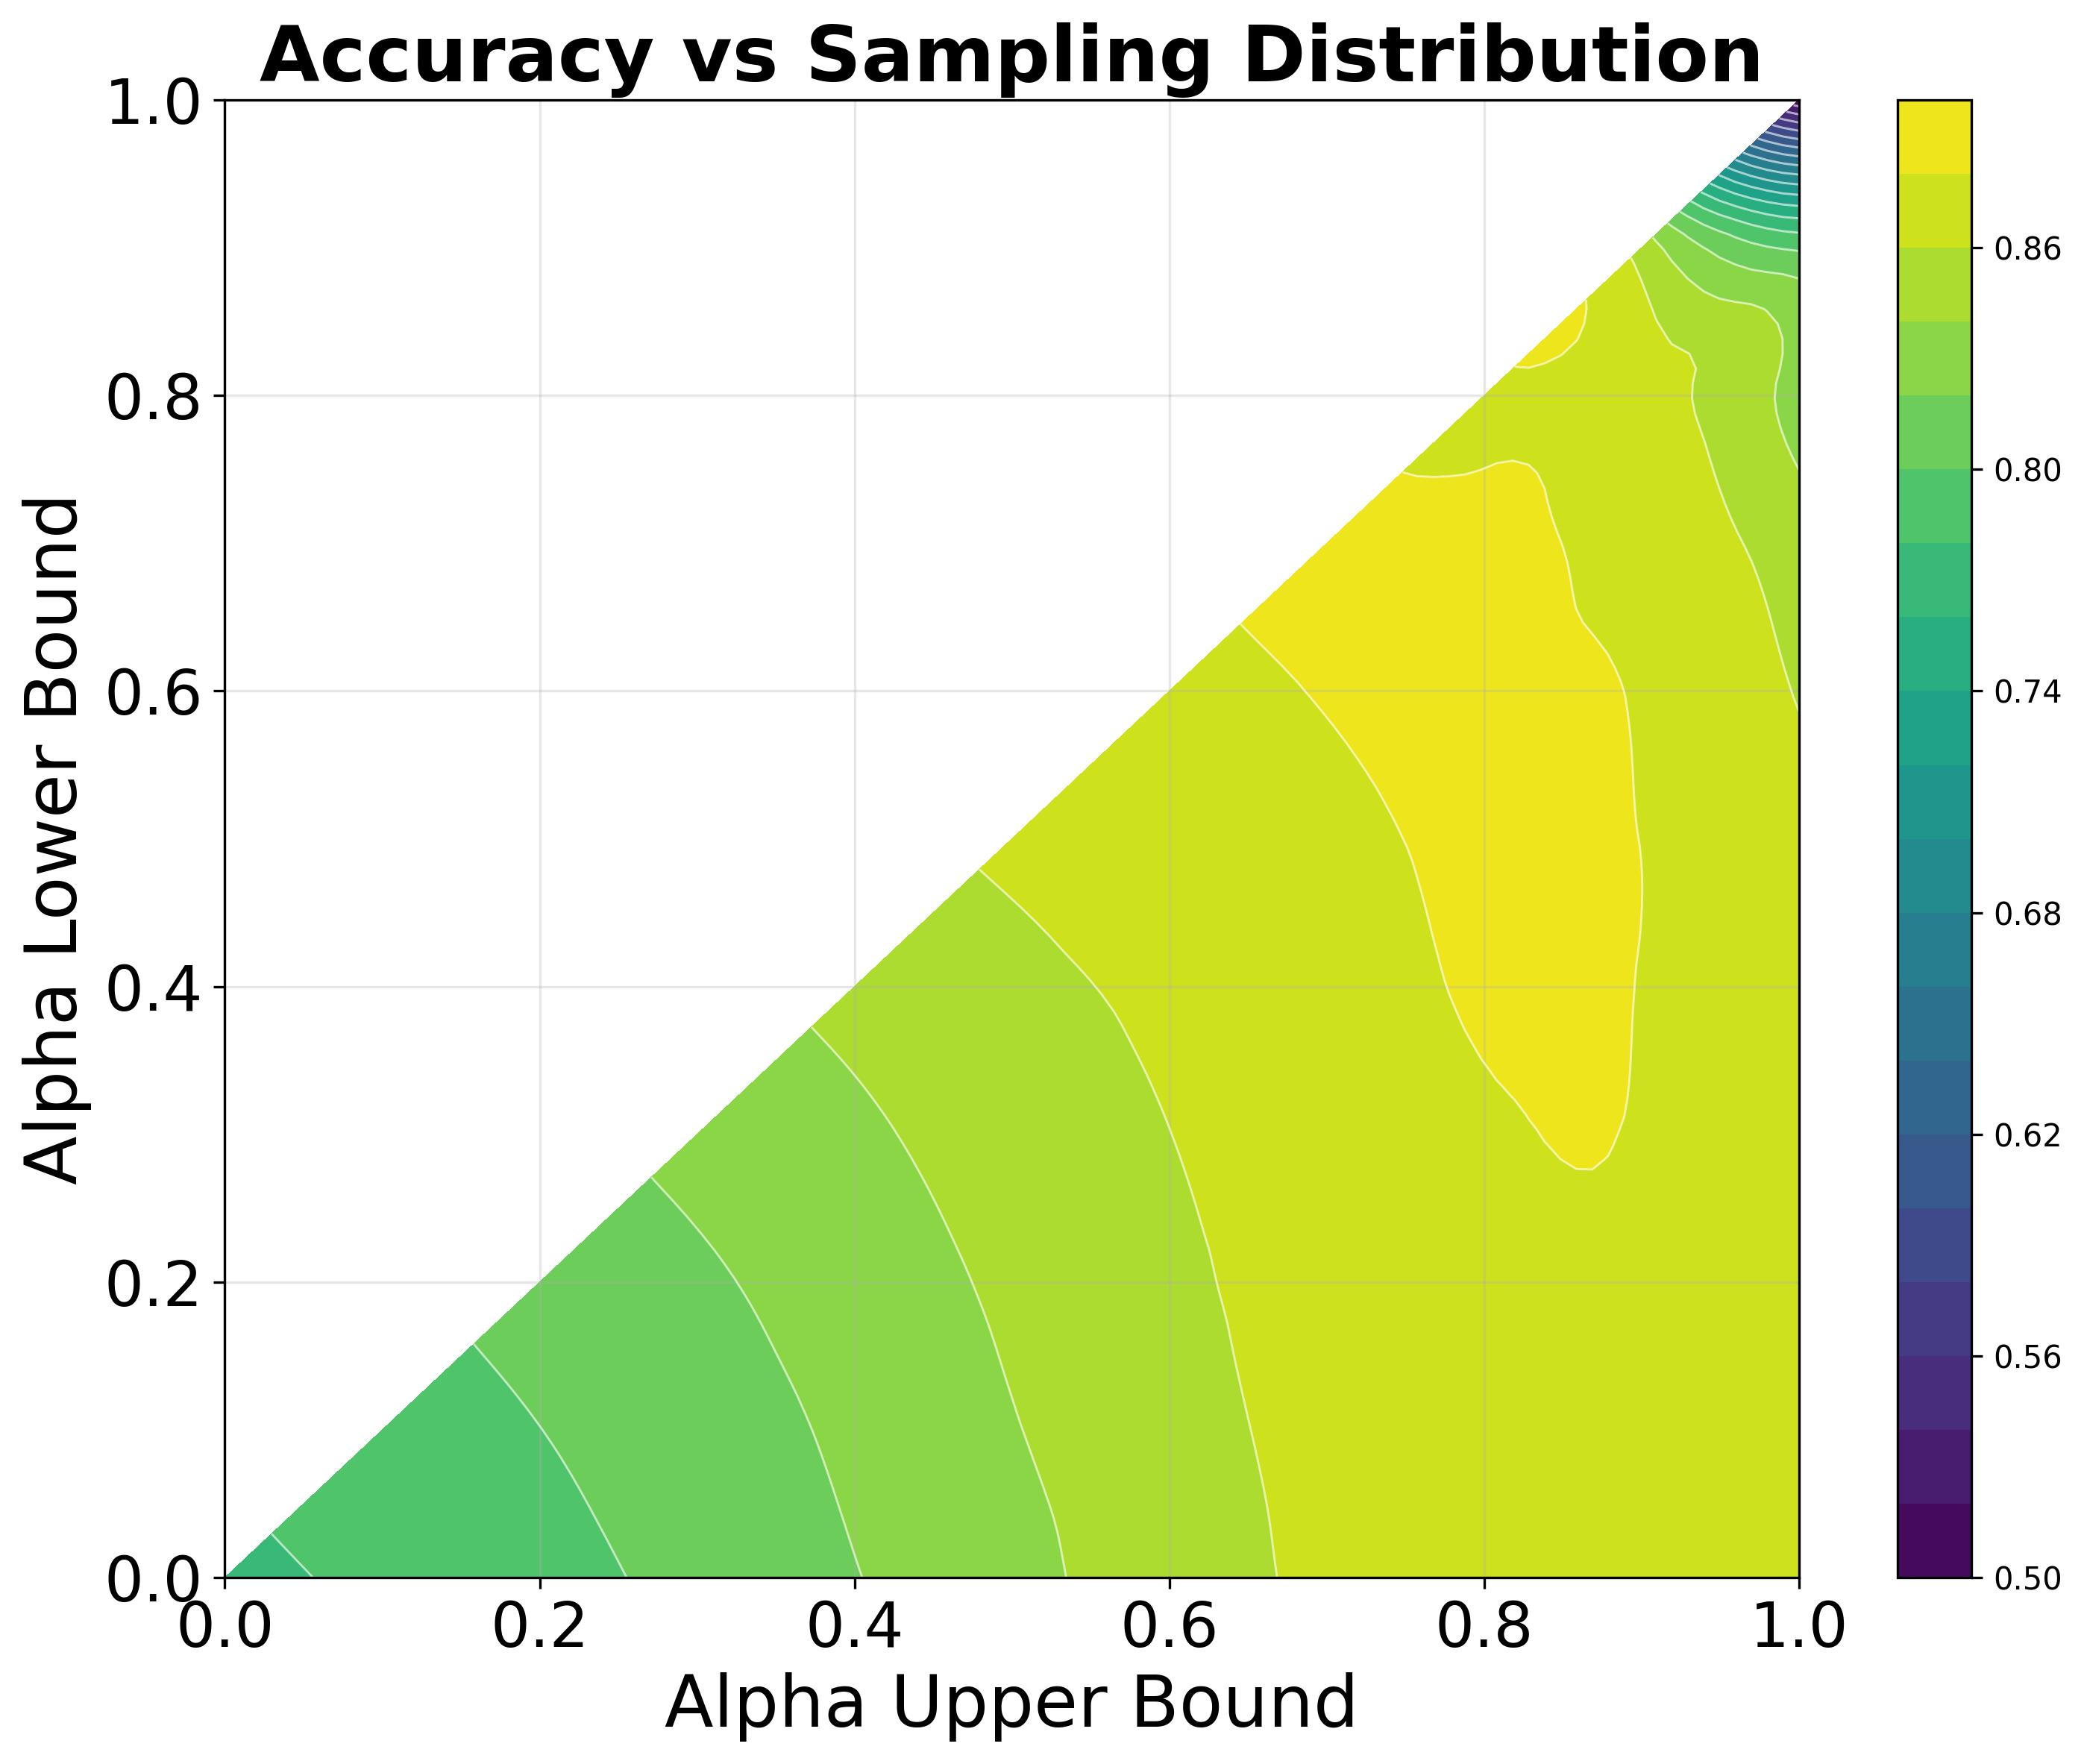
\includegraphics[width=\linewidth]{proposal/images/simlbr/alpha_ablation.jpeg}\\
  {\small (a)}
\end{minipage}\hfill
\begin{minipage}[t]{0.48\linewidth}
  \centering
  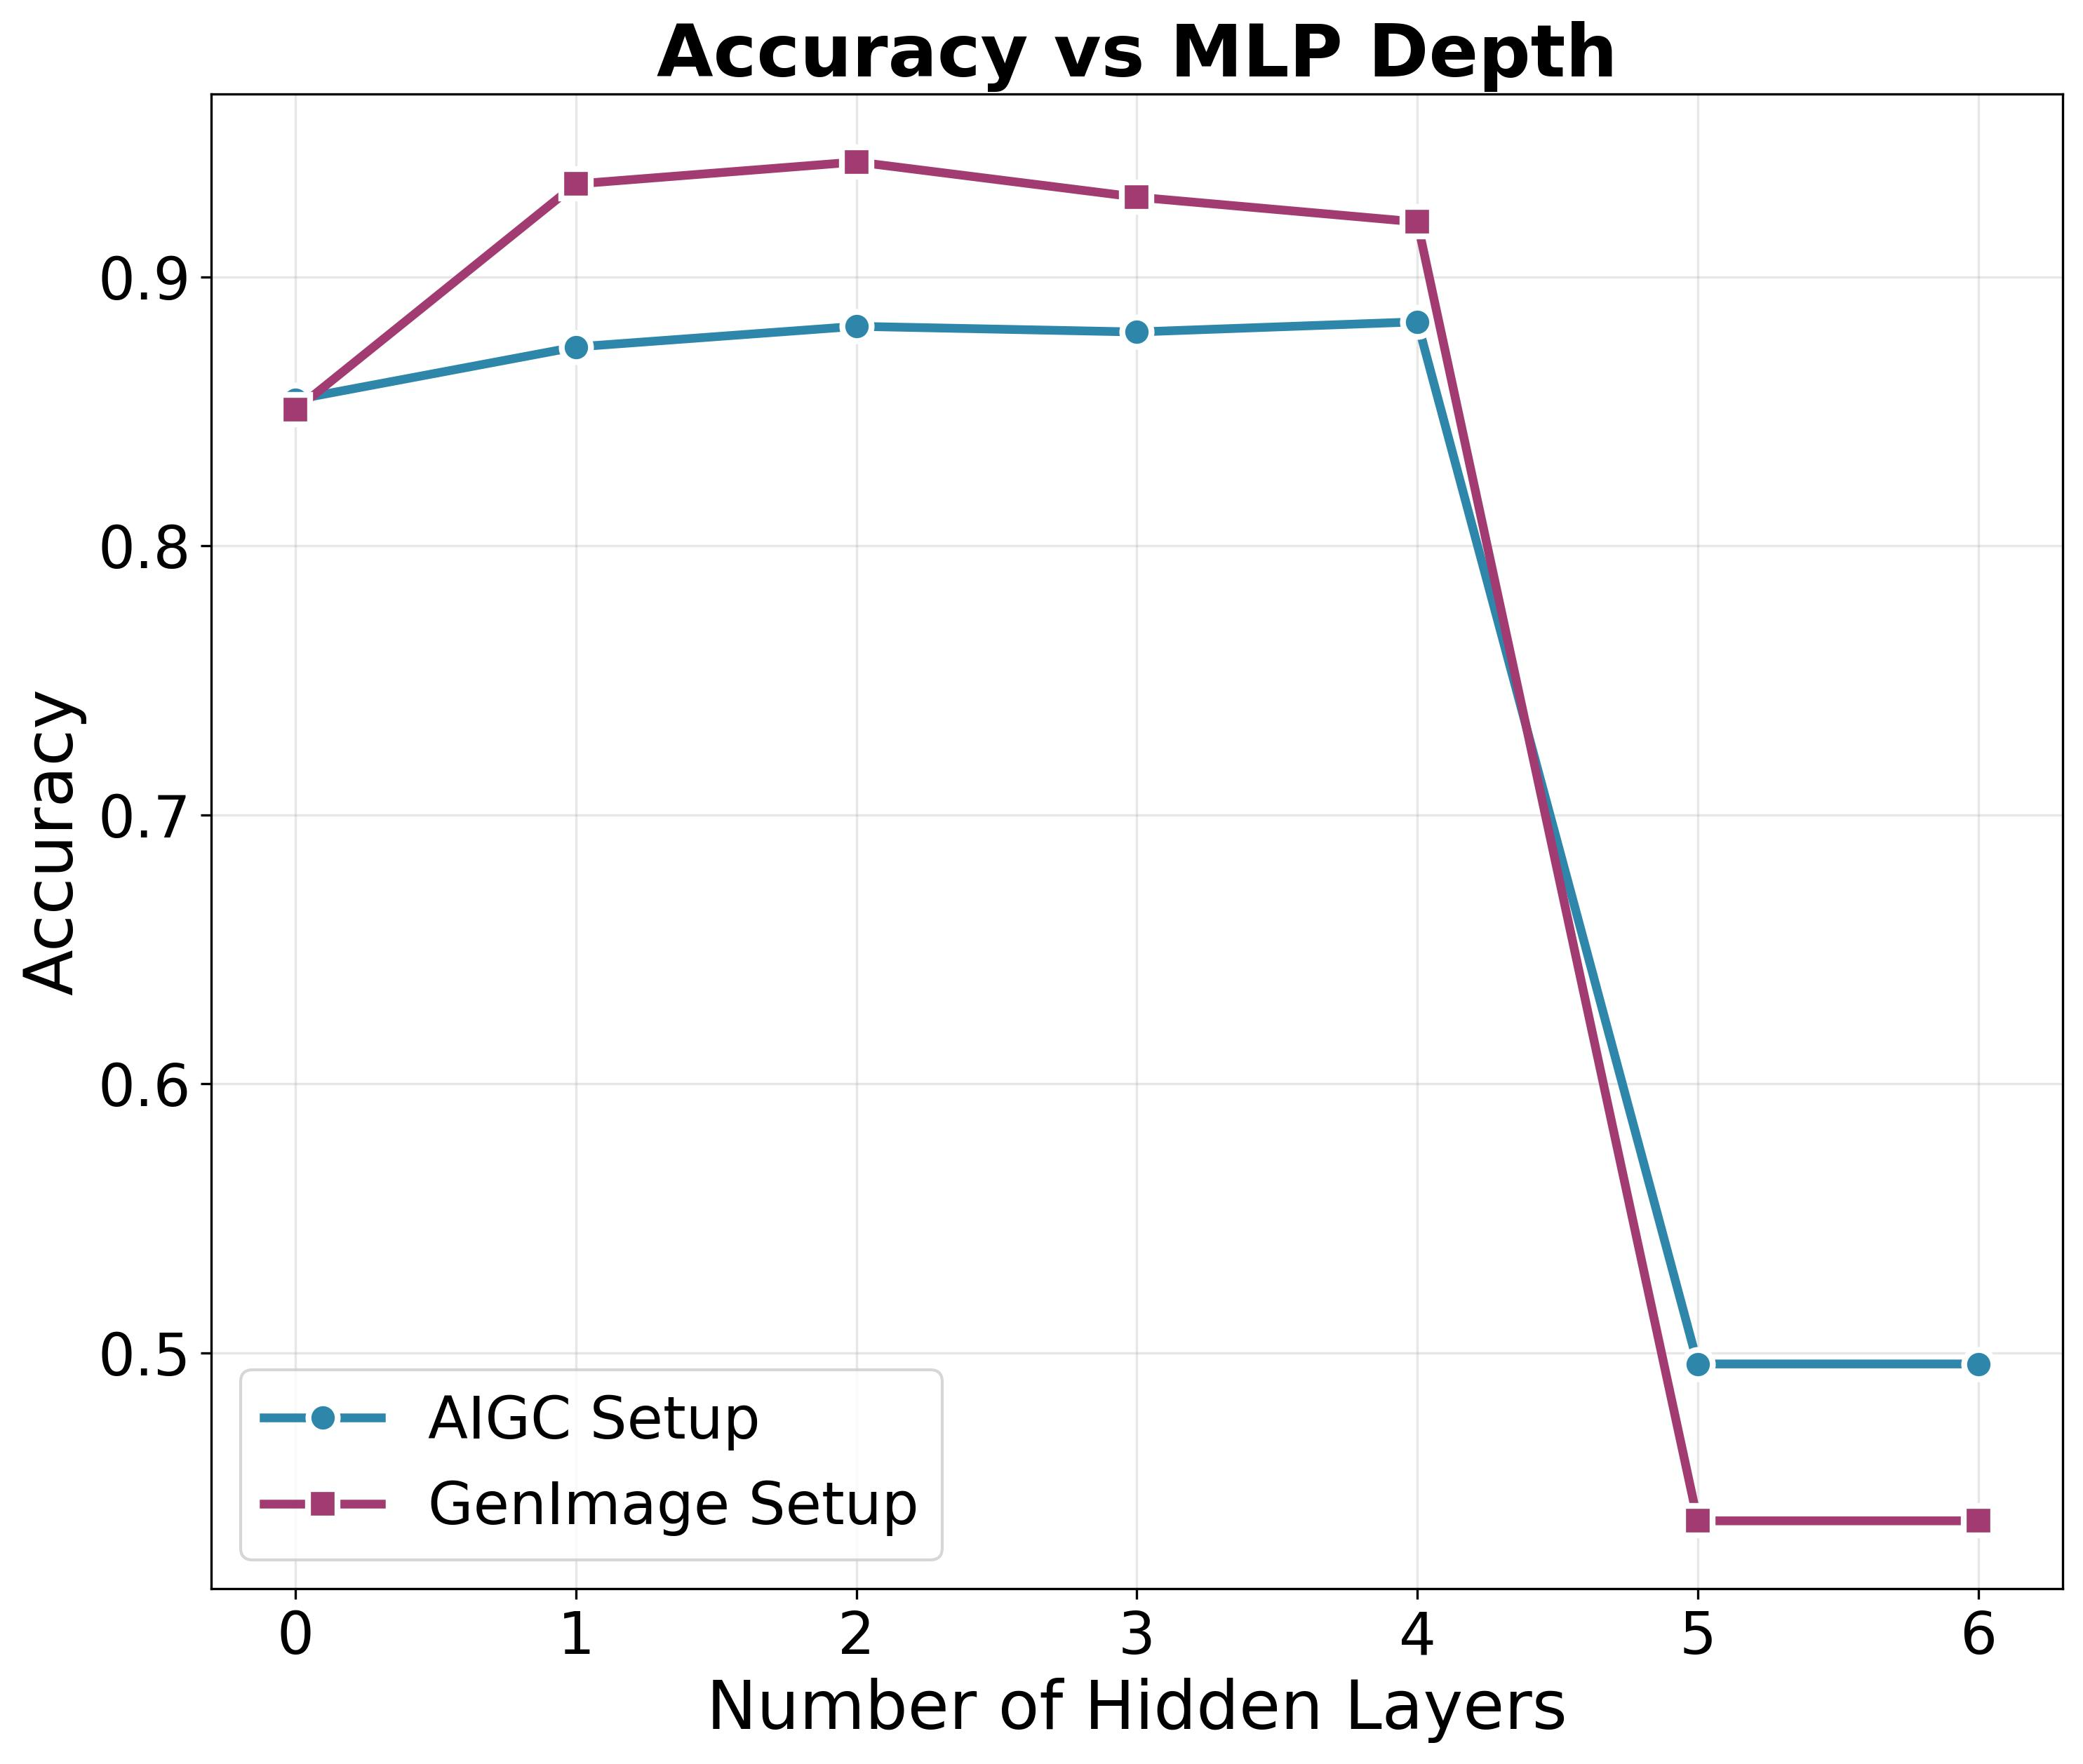
\includegraphics[width=\linewidth]{proposal/images/simlbr/depth_ablation.jpeg}\\
  {\small (b)}
\end{minipage}
\caption{\textbf{(a) Ablation of the sampling distribution for $\alpha$:} SimLBR is trained on ProGAN with different sampling distributions for $\alpha$. Always retaining at least half of the information from the real image is an optimal and robust choice. \textbf{(b) Ablation of MLP depth:} SimLBR performs better with smaller MLPs and overfits when the MLP has many hidden layers.}
\label{fig:simlbr_alpha_depth}
\end{figure}

\subsubsection{Ablation Studies}
\label{sec:simlbr_ablation}
\noindent\textbf{Impact of LBR and the latent space:} To isolate the contribution of latent blending regularization, we train a baseline MLP under an identical setup without LBR. To understand the role of the latent space, we also train models on features from the older DINOv2~\cite{oquab2024dinov2}. In addition to Chameleon, AIGC, and GenImage, this ablation includes RSFake-1M, which lets us evaluate the effect of LBR under a large shift in the image distribution. Since a satellite-specific DINOv2 is not available, RSFake-1M is evaluated only with the DINOv3 backbone. Table~\ref{table:simlbr_ablate} summarizes the results. Adding LBR in the DINOv3 latent space yields an average accuracy gain of $10.21\%$. The effect is even more pronounced for fake image accuracy, which improves from $7.24\%$ to $75.80\%$ on Chameleon (ProGAN), $54.07\%$ to $82.07\%$ on AIGC, $89.03\%$ to $92.96\%$ on Chameleon (SD v1.4), $85.80\%$ to $93.89\%$ on GenImage, and $48.28\%$ to $78.87\%$ on RSFake-1M, an average increase of over 25 percentage points. On RSFake-1M, the overall accuracy improves from $73.90\%$ to $88.88\%$, showing that LBR is equally effective for generated satellite imagery. LBR also substantially reduces the standard deviation across settings and improves the reliability and worst-case estimates.

Interestingly, LBR does not yield the same improvements in the DINOv2 latent space. LBR operates entirely in the latent space by injecting small amounts of fake information into real image latents. This assumes a geometrically smooth manifold, on which such interpolation yields a smooth change that stays on the valid embedding manifold. We hypothesize that the lack of improvement with DINOv2 is related to limitations in the manifold structure of weaker embedding models~\cite{kang2025clip,li2025lost,liu2024assessing}.

\noindent\textbf{In-distribution vs.\ out-of-distribution generators:} Detectors generally perform better on generators that share architectural similarities with the training generator, because these generators produce similar artifacts~\cite{zhu2023genimage,yansanity}. To further isolate the contribution of LBR, we partition the test generators into in-distribution (ID) and out-of-distribution (OD) groups. For AIGC, which is trained on ProGAN, GAN-based generators are ID and diffusion-based generators are OD; for GenImage, which is trained on Stable Diffusion, the assignment is reversed. Table~\ref{table:simlbr_idod} shows that LBR yields modest gains on ID generators, where the baseline already performs well, but large gains on OD generators ($10.30\%$ on GenImage and $12.72\%$ on AIGC). This shows that LBR helps the detector generalize beyond artifact-level correlations to previously unseen generative architectures.

\noindent\textbf{Sampling distribution for $\alpha$:} Figure~\ref{fig:simlbr_alpha_depth}(a) shows how different sampling strategies for $\alpha$ affect performance. Consistent with our hypothesis, sampling only low values of $\alpha$ leads to poor performance, since injecting excessive fake information makes the task trivial. Sampling only high values of $\alpha$ also degrades performance sharply, because the perturbed samples become nearly identical to unperturbed real images, which makes the regularization too strong. Sampling from $\text{Uniform}(0.5, B)$ balances these extremes, and the method is robust to the choice of $B$, with values in the range $0.7 < B < 0.9$ consistently yielding the best performance.

\noindent\textbf{MLP depth:} Figure~\ref{fig:simlbr_alpha_depth}(b) shows that SimLBR performs well with 0 to 4 hidden layers, but deteriorates rapidly beyond 4 layers, as larger MLPs overfit to the training data.

\noindent\textbf{Comparison to anomaly detection:} We train a One-Class SVM with an RBF kernel on DINOv3 features of the real training images, sweeping $\nu$ to find the best value. The OC-SVM performs substantially worse than SimLBR on both AIGC and GenImage. Modern generators produce photorealistic images whose latent representations lie close to those of real images, so learning the support of the real distribution alone is insufficient. SimLBR instead uses controlled amounts of fake information to shape a meaningful boundary around the real-image manifold. \todo{Decide whether to include the OC-SVM figures (proposal/images/simlbr/ocsvm\_aigc.png and ocsvm\_genimage.png) and report their numbers here.}

\noindent\textbf{Visualizing the learned embeddings:} Figure~\ref{fig:simlbr_tsne} shows t-SNE visualizations of the penultimate-layer embeddings of detectors trained on ProGAN with and without LBR. Without LBR, the detector overfits to the training fakes and does not preserve a meaningful separation between real and fake distributions; there is even a clear separation between the train and test real images. With LBR, the real images form a compact cluster, and fake images from the unseen generator fall outside it.

\subsection{Structured Latent Blending Regularization}
\label{sec:structured_lbr}
SimLBR constructs each pseudo-fake by moving a real embedding along a single direction, the line from $L^R$ to $L^F$, by a single scalar amount $\alpha$. As a result, the set of pseudo-fakes that can be created from a given real-fake pair is a line segment. In this section, we describe extensions of SimLBR that we developed after its publication. Each extension creates harder and more diverse pseudo-fakes by perturbing the real embedding along a richer set of directions. \todo{Add context: where and when this work was done (internship), collaborators, and its publication status.}

\noindent\textbf{Motivation:} LBR aims to create pseudo-fakes that lie just outside the real distribution. However, it does so by moving the global summary vector of the entire real image toward a fake. Any perturbation of the summary vector could move the latent significantly away from the real image distribution, making the pseudo-fake too easy to detect. One natural alternative, which we call Localized Latent Blending Regularization (LLBR), is to perturb only the local (patch-level) feature vectors rather than the summary vector, producing harder pseudo-fakes. \todo{State whether LLBR experiments were run and what they showed.} The geometric intuition behind LLBR is that the pseudo-fakes are created by moving along more diverse directions. This raises the question of whether the same intuition can be applied directly in the space of the global (CLS) representation, by perturbing only a subset of its dimensions.

\begin{figure}[!t]
\centering
\begin{minipage}[t]{0.52\linewidth}
  \centering
  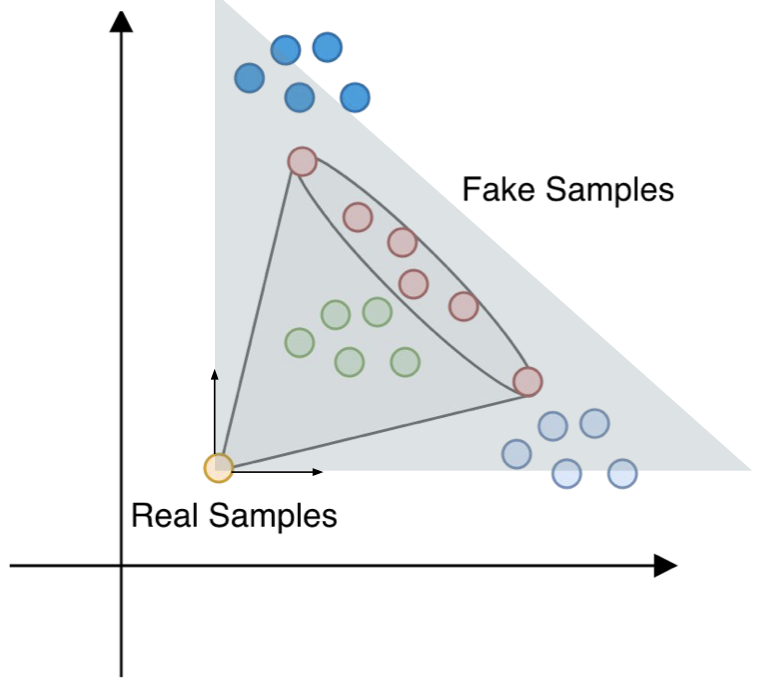
\includegraphics[width=\linewidth]{proposal/images/simlbr/plbr_geometry.png}\\
  {\small (a)}
\end{minipage}\hfill
\begin{minipage}[t]{0.42\linewidth}
  \centering
  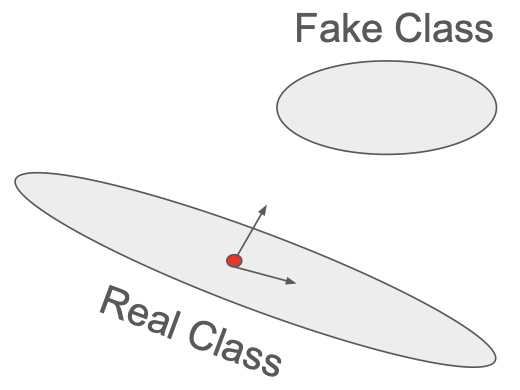
\includegraphics[width=\linewidth]{proposal/images/simlbr/pca_lbr_schematic.png}\\
  {\small (b)}
\end{minipage}
\caption{\textbf{Geometric intuition for structured LBR:} (a) SimLBR creates pseudo-fakes along the line segment between a real sample (yellow) and a fake sample (red). Perturbing different subsets of dimensions with different amounts expands the set of reachable pseudo-fakes (green) from a line segment to a larger region, covering more of the space in which unseen fakes (blue) may lie. (b) In a PCA basis of the real class, we know which directions have high and low variance, and can choose which directions to perturb. \todo{Redraw both panels for the dissertation; these are taken from presentation slides.}}
\label{fig:structured_lbr}
\end{figure}

\subsubsection{Partial Latent Blending Regularization (P-LBR)}
In Partial LBR, we blend only a subset of the dimensions of the latent representation. Let $d$ be the dimension of the representation, and let $\mathcal{S} \subset \{1, \ldots, d\}$ be a randomly sampled subset of $k$ dimensions. We define a per-dimension blending vector $\boldsymbol{\alpha} \in \mathbb{R}^d$ as:
\begin{equation}
\alpha_j =
\begin{cases}
\alpha, & j \in \mathcal{S}\\
1, & j \notin \mathcal{S}
\end{cases}
\qquad \alpha \sim \text{Uniform}(a, B)
\label{eq:plbr_alpha}
\end{equation}
The pseudo-fake representation is then computed as:
\begin{equation}
L_i = \boldsymbol{\alpha} \odot L_i^{R} + (\mathbf{1}-\boldsymbol{\alpha}) \odot L_i^{F}
\label{eq:plbr}
\end{equation}
where $\odot$ is the element-wise product. Dimensions outside $\mathcal{S}$ are copied unchanged from the real representation. SimLBR is the special case $k=d$. As illustrated in Figure~\ref{fig:structured_lbr}(a), because a different subset of dimensions is perturbed for each sample, the pseudo-fakes are no longer restricted to the line between $L^R$ and $L^F$. \todo{Confirm: the embedding dimension $d$, whether $\mathcal{S}$ is resampled for every training sample, and the final values of $k$, $a$, and $B$ (the best run used $k=712$, $\alpha \sim \text{Uniform}(0.6, 0.8)$, and weight decay \texttt{5e-3}).}

\subsubsection{Independent Latent Blending Regularization (I-LBR)}
P-LBR allows movement along only a subset of dimensions. In Independent LBR, we allow movement along all dimensions, but each dimension is blended by an independently sampled amount:
\begin{equation}
\alpha_j \sim \text{Uniform}(a, B) \quad \text{independently for } j = 1, \ldots, d
\label{eq:ilbr_alpha}
\end{equation}
with the pseudo-fake computed using Equation~\ref{eq:plbr}. This expands the feasible set of pseudo-fakes for a given real-fake pair from a line segment (SimLBR) to an axis-aligned hyperrectangle. The feasible set of pseudo-fakes from P-LBR is a subset of the feasible set of I-LBR when the same range of $\alpha$ is used. \todo{Confirm the final I-LBR configuration (the best run used $\alpha_j \sim \text{Uniform}(0.75, 0.8)$, weight decay \texttt{5e-3}, and a plateau learning-rate schedule).}

\subsubsection{PCA Latent Blending Regularization (PCA-LBR)}
Both P-LBR and I-LBR show that there is value in perturbing different dimensions by different amounts (Section~\ref{sec:structured_lbr_results}). However, they still rely on randomness to choose which dimensions to perturb. In PCA-LBR, we instead choose the perturbation directions using the structure of the data. We transform the representations to a new basis using PCA. In this basis, we know the directions of most and least variance of the data, and we use this information to decide which directions should be perturbed (Figure~\ref{fig:structured_lbr}(b)). Specifically:
\begin{enumerate}
    \item We compute supervised PCA between the real and fake classes and obtain the most discriminative direction $v_0$.
    \item We project the real data onto the orthogonal complement of $v_0$, i.e., we remove the $v_0$ component.
    \item We perform PCA on the projection of the real class onto $\text{span}\{v_0\}^\perp$, completing a basis $\mathcal{B} = \{v_0, v_1, \ldots, v_{d-1}\}$ with change-of-basis matrix $B$, where $v_1, \ldots, v_{d-1}$ are ordered by decreasing variance.
    \item We apply $B$ to all representations.
    \item For each real-fake pair $(r, f)$ in the new basis, we blend the coordinates for $v_0$ and for the $m$ lowest-variance directions $v_{d-m}, \ldots, v_{d-1}$. Let $\alpha_j^{\text{PCA}} = \alpha$ if $v_j$ is a direction to perturb and $\alpha_j^{\text{PCA}} = 1$ otherwise. The pseudo-fake is:
    \begin{equation}
    \boldsymbol{\alpha}^{\text{PCA}} \odot r + (\mathbf{1} - \boldsymbol{\alpha}^{\text{PCA}}) \odot f
    \label{eq:pcalbr}
    \end{equation}
    and it is labeled as fake. The classifier is trained in the space with basis $\mathcal{B}$.
\end{enumerate}
Perturbing the low-variance directions of the real class creates pseudo-fakes that leave the real distribution along directions in which real images rarely vary, which should make them both close to the real distribution and clearly distinct from it. \todo{Confirm: what ``supervised PCA'' refers to exactly, and the final number of perturbed directions $m$ for the PCA-PLBR results (runs are labeled ``partial712d-randomordered'').}

\begin{table}[!t]
\centering
\small
\begin{tabular}{l|ccc}
\hline
Generator & SimLBR & P-LBR & PCA-PLBR \\
\hline
ProGAN (Training) & 99.24 & \textbf{99.29} & 99.24 \\
\hline
StyleGAN   & 88.66 & 88.92 & \textbf{89.54} \\
BigGAN     & 95.75 & 95.30 & \textbf{95.80} \\
CycleGAN   & 89.36 & 88.19 & \textbf{90.84} \\
StarGAN    & 89.27 & \textbf{89.69} & 87.47 \\
GauGAN     & 96.98 & 97.06 & \textbf{97.52} \\
StyleGAN2  & 85.67 & 87.01 & \textbf{87.29} \\
WFIR       & 89.25 & \textbf{90.70} & 90.35 \\
ADM        & 85.81 & 86.08 & \textbf{86.85} \\
Glide      & 90.53 & 91.38 & \textbf{91.72} \\
Midjourney & 74.55 & \textbf{76.56} & 74.30 \\
SD v1.4    & 84.95 & \textbf{86.34} & 85.09 \\
SD v1.5    & 84.16 & \textbf{85.25} & 84.08 \\
VQDM       & 93.25 & 92.71 & \textbf{93.59} \\
Wukong     & 90.23 & \textbf{90.70} & 90.12 \\
DALLE2     & 79.80 & \textbf{82.65} & 81.20 \\
\hline
\textit{Mean}$\uparrow$        & 88.59 & \textbf{89.24} & 89.06 \\
\textit{Std}$\downarrow$         & 6.26 & \textbf{5.57} & 6.25 \\
\textit{Reliability}$\uparrow$ & 6.16 & \textbf{7.05} & 6.25 \\
\textit{WCE}$\uparrow$         & 74.55 & \textbf{76.56} & 74.30 \\
\hline
\end{tabular}
\caption{\textbf{Structured LBR on AIGC:} Accuracy of detectors trained on ProGAN. The SimLBR column is our re-run of SimLBR under the same setup as the structured variants. P-LBR improves mean accuracy, reliability, and the worst-case estimate over SimLBR. \todo{Explain why the re-run SimLBR mean (88.59) differs slightly from the published value (88.40).}}
\label{table:structured_aigc}
\end{table}

\begin{table}[!t]
\centering
\small
\begin{tabular}{l|cc}
\hline
Generator & SimLBR & PCA-PLBR \\
\hline
SD v1.4 (Training) & \textbf{97.54} & 97.23 \\
\hline
Midjourney & 92.46 & \textbf{92.52} \\
SD v1.5    & \textbf{97.66} & 97.26 \\
ADM        & \textbf{96.15} & 95.43 \\
GLIDE      & 92.95 & \textbf{93.48} \\
Wukong     & \textbf{97.24} & 96.88 \\
VQDM       & 93.74 & \textbf{94.14} \\
BigGAN     & 88.94 & \textbf{90.65} \\
\hline
\textit{Mean}$\uparrow$        & 94.59 & \textbf{94.70} \\
\textit{Std}$\downarrow$         & 3.10 & \textbf{2.43} \\
\textit{Reliability}$\uparrow$ & 14.36 & \textbf{18.41} \\
\textit{WCE}$\uparrow$         & 88.94 & \textbf{90.65} \\
\hline
\end{tabular}
\caption{\textbf{Structured LBR on GenImage:} Accuracy of detectors trained on Stable Diffusion v1.4. PCA-PLBR improves the accuracy on the most out-of-distribution generator, BigGAN, which reduces the variance across generators and improves the reliability and worst-case estimate.}
\label{table:structured_genimage}
\end{table}

\begin{table}[!t]
\centering
\begin{tabular}{l|ccc}
\hline
Method & Accuracy & Real Acc. & Fake Acc. \\
\hline
SimLBR       & 84.33 & 90.74 & 75.80 \\
P-LBR        & 83.84 & 89.30 & \textbf{76.58} \\
PCA-PLBR     & \textbf{84.92} & \textbf{92.98} & 74.19 \\
\hline
\end{tabular}
\caption{\textbf{Structured LBR on Chameleon:} Detectors are trained on ProGAN.}
\label{table:structured_chameleon}
\end{table}

\subsubsection{Experiments and Results}
\label{sec:structured_lbr_results}
We follow the experimental setup of SimLBR and train all variants on DINOv3 features. During development, we compared variants by their validation accuracy when trained on AIGC (ProGAN). \todo{Specify which validation split was used for model selection.}

\noindent\textbf{Development experiments:} Perturbing a random subset of $512$ dimensions with P-LBR did not improve over SimLBR (peak validation accuracy of approximately $88.0\%$ for both). Increasing the subset to $704$ or $712$ dimensions improved the peak validation accuracy to approximately $88.4\%$. Narrowing the sampling range of $\alpha$ to $\text{Uniform}(0.6, 0.8)$ and reducing the weight decay to \texttt{5e-3} further improved it to approximately $88.7\%$, our best P-LBR configuration. I-LBR reached a similar peak validation accuracy of approximately $88.7\%$, without a clear advantage over P-LBR. \todo{Replace the approximate values read from the training curves with the exact logged numbers.}

\noindent\textbf{Low-variance vs.\ high-variance directions:} To test the intuition behind PCA-LBR, we reversed the selection and perturbed the \textit{highest}-variance directions instead of the lowest. Perturbing low-variance directions was consistently better: with 256 perturbed directions, the peak validation accuracy was approximately $87.4\%$ for low-variance directions vs.\ $86.9\%$ for high-variance directions; with 512 directions, approximately $87.5\%$ vs.\ $87.2\%$; and with 712 directions, approximately $88.4\%$ vs.\ $88.3\%$. This supports the hypothesis that pseudo-fakes are more useful when they leave the real distribution along directions in which real images rarely vary.

\noindent\textbf{AIGC:} Table~\ref{table:structured_aigc} reports the full evaluation on AIGC. P-LBR improves the mean accuracy from $88.59\%$ to $89.24\%$ and gives the largest improvements on generators where SimLBR is weakest, such as DALLE2 ($+2.85\%$), Midjourney ($+2.01\%$), and Stable Diffusion v1.4 ($+1.39\%$). As a result, P-LBR reduces the standard deviation from $6.26$ to $5.57$, improves the reliability from $6.16$ to $7.05$, and raises the worst-case estimate from $74.55\%$ to $76.56\%$. PCA-PLBR improves the mean accuracy to $89.06\%$, with gains on most GAN-based generators, but does not improve the worst-case estimate.

\noindent\textbf{GenImage:} Table~\ref{table:structured_genimage} compares SimLBR and PCA-PLBR on GenImage. The mean accuracy is nearly unchanged ($94.59\%$ vs.\ $94.70\%$), but PCA-PLBR improves the accuracy on BigGAN, the generator most different from the training generator, from $88.94\%$ to $90.65\%$. This reduces the standard deviation from $3.10$ to $2.43$ and improves the reliability from $14.36$ to $18.41$.

\noindent\textbf{Chameleon:} Table~\ref{table:structured_chameleon} shows the results on Chameleon. PCA-PLBR achieves the highest overall accuracy ($84.92\%$), driven by better real-image accuracy ($92.98\%$), while P-LBR achieves the highest fake-image accuracy ($76.58\%$).

\noindent\textbf{Discussion:} The structured variants of LBR give consistent but modest improvements over SimLBR. The improvements in mean accuracy are under one percentage point, but they are concentrated on the hardest, most out-of-distribution generators, which translates into larger improvements in reliability and in the worst-case estimate. This supports the geometric intuition that moving real embeddings along more diverse, and more carefully chosen, directions produces pseudo-fakes that better define the boundary of the real distribution. A natural next step is to select the perturbed directions and their blending amounts using the eigenvalues of the real class, rather than a fixed number of lowest-variance directions.


\subsection{Proposed Direction}
In this section, we outline the next steps planned for this chapter. In Section~\ref{sec:few-shot}, we conducted few-shot learning experiments on geospatial deepfakes and proposed two hypotheses from the results. We plan to validate these hypotheses with experimental results. For H1, we will design visualization pipelines to inspect the artifacts in the deepfake qualitatively. For H2, we will utilize the representations extracted from deepfakes to train downstream models and investigate how this impacts performance when compared to using uncorrupted training data. 

In Section~\ref{sec:seperability}, we proposed a new metric, $Seperability@K$, to measure the presence of artifacts in deepfakes. We will compute this metric for the state-of-the-art geospatial generative models. We will rank the models based on our metric and analyze the correlation with other generative metrics such as LPIPS and FID scores. 

In Section~\ref{sec:simlbr}, we presented SimLBR, a simple and efficient framework for generalizable fake image detection that learns a tight decision boundary around the real image distribution using latent blending regularization, and in Section~\ref{sec:structured_lbr}, we extended it with structured perturbations that move real embeddings along more diverse and more carefully chosen directions. A remaining direction is to use SimLBR as a feedback mechanism for generative models to improve the $Separability$ score of these models. A better generative model can feed into pretraining pipelines to scale and learn richer and more generalizable representations. \todo{Update this section once the status of the few-shot hypotheses, the Separability metric, soft-label learning, and the generative-model feedback work is decided.}

\subsection{Chapter Conclusion}
In summary, these are the major tasks required to complete this chapter:
\begin{itemize}
    \item Design a framework to validate the hypotheses offered in Section~\ref{sec:few-shot}.
    \item Run experiments to compute $ Separability$ scores for state-of-the-art models. Validate the utility of our proposed metrics.
    \item Develop SimLBR, a generalizable fake image detector based on latent blending regularization, and extend it with structured latent blending (Sections~\ref{sec:simlbr} and~\ref{sec:structured_lbr}). \textit{(Completed.)}
    \item Work towards using the results from this chapter to improve geospatial generative models and feed good quality data to improve representation learning pipelines.
\end{itemize}
\newpage
\section{Timeline}
\begin{table}[!h]
\resizebox{\linewidth}{!}{
\begin{tabular}{llllllllllllllll}
\hline
 \multicolumn{1}{|l|}{} & \multicolumn{8}{c|}{2025}                                                                                                                                                                                                                   & \multicolumn{7}{c|}{2026}                                                           \\
\hline
\multicolumn{1}{|l|}{}                                                                                    & \multicolumn{1}{l|}{May} & \multicolumn{1}{l|}{Jun} & \multicolumn{1}{l|}{Jul} & \multicolumn{1}{l|}{Aug} & \multicolumn{1}{l|}{Sep} & \multicolumn{1}{l|}{Oct} & \multicolumn{1}{l|}{Nov}                      & \multicolumn{1}{l|}{Dec} & \multicolumn{1}{l|}{Jan} & \multicolumn{1}{l|}{Feb} & \multicolumn{1}{l|}{Mar} & \multicolumn{1}{l|}{Apr} & \multicolumn{1}{l|}{May} & \multicolumn{1}{l|}{Jun} & \multicolumn{1}{l|}{Jul} \\ \hline
\multicolumn{1}{|l|}{Internship}                                                                          & \multicolumn{4}{l|}{\cellcolor[HTML]{FFCE93}}                                                             & \multicolumn{1}{l|}{}    & \multicolumn{1}{l|}{}    & \multicolumn{1}{l|}{}                         & \multicolumn{1}{l|}{}    & \multicolumn{1}{l|}{}    & \multicolumn{1}{l|}{}    & \multicolumn{1}{l|}{}    & \multicolumn{1}{l|}{}    & \multicolumn{1}{l|}{}    & \multicolumn{1}{l|}{}    & \multicolumn{1}{l|}{}    \\ \hline
\multicolumn{1}{|l|}{Few-shot experiments}                                                                & \multicolumn{1}{l|}{}    & \multicolumn{1}{l|}{}    & \multicolumn{3}{l|}{\cellcolor[HTML]{CBCEFB}}                                  & \multicolumn{1}{l|}{}    & \multicolumn{1}{l|}{}                         & \multicolumn{1}{l|}{}    & \multicolumn{1}{l|}{}    & \multicolumn{1}{l|}{}    & \multicolumn{1}{l|}{}    & \multicolumn{1}{l|}{}    & \multicolumn{1}{l|}{}    & \multicolumn{1}{l|}{}    & \multicolumn{1}{l|}{}    \\ \hline
\multicolumn{1}{|l|}{Initial SimDLR framework}                                                            & \multicolumn{1}{l|}{}    & \multicolumn{1}{l|}{}    & \multicolumn{1}{l|}{}    & \multicolumn{2}{l|}{\cellcolor[HTML]{CBCEFB}}       & \multicolumn{1}{l|}{}    & \multicolumn{1}{l|}{}                         & \multicolumn{1}{l|}{}    & \multicolumn{1}{l|}{}    & \multicolumn{1}{l|}{}    & \multicolumn{1}{l|}{}    & \multicolumn{1}{l|}{}    & \multicolumn{1}{l|}{}    & \multicolumn{1}{l|}{}    & \multicolumn{1}{l|}{}    \\ \hline
\multicolumn{1}{|l|}{Work on dissertation proposal}                                                       & \multicolumn{1}{l|}{}    & \multicolumn{1}{l|}{}    & \multicolumn{1}{l|}{}    & \multicolumn{3}{l|}{\cellcolor[HTML]{FFFFC7}}                                  & \multicolumn{1}{l|}{}                         & \multicolumn{1}{l|}{}    & \multicolumn{1}{l|}{}    & \multicolumn{1}{l|}{}    & \multicolumn{1}{l|}{}    & \multicolumn{1}{l|}{}    & \multicolumn{1}{l|}{}    & \multicolumn{1}{l|}{}    & \multicolumn{1}{l|}{}    \\ \hline
\multicolumn{1}{|l|}{Seperability metric}                                                                 & \multicolumn{1}{l|}{}    & \multicolumn{1}{l|}{}    & \multicolumn{1}{l|}{}    & \multicolumn{1}{l|}{}    & \multicolumn{3}{l|}{\cellcolor[HTML]{CBCEFB}}                                                       & \multicolumn{1}{l|}{}    & \multicolumn{1}{l|}{}    & \multicolumn{1}{l|}{}    & \multicolumn{1}{l|}{}    & \multicolumn{1}{l|}{}    & \multicolumn{1}{l|}{}    & \multicolumn{1}{l|}{}    & \multicolumn{1}{l|}{}    \\ \hline
\multicolumn{1}{|l|}{\begin{tabular}[c]{@{}l@{}}Experimental validation of\\ hypotheses\end{tabular}}     & \multicolumn{1}{l|}{}    & \multicolumn{1}{l|}{}    & \multicolumn{1}{l|}{}    & \multicolumn{1}{l|}{}    & \multicolumn{1}{l|}{}    & \multicolumn{2}{l|}{\cellcolor[HTML]{CBCEFB}}                            & \multicolumn{1}{l|}{}    & \multicolumn{1}{l|}{}    & \multicolumn{1}{l|}{}    & \multicolumn{1}{l|}{}    & \multicolumn{1}{l|}{}    & \multicolumn{1}{l|}{}    & \multicolumn{1}{l|}{}    & \multicolumn{1}{l|}{}    \\ \hline
\multicolumn{1}{|l|}{New adjustments to SimDLR}                                                           & \multicolumn{1}{l|}{}    & \multicolumn{1}{l|}{}    & \multicolumn{1}{l|}{}    & \multicolumn{1}{l|}{}    & \multicolumn{1}{l|}{}    & \multicolumn{4}{l|}{\cellcolor[HTML]{CBCEFB}}                                                                                  & \multicolumn{1}{l|}{}    & \multicolumn{1}{l|}{}    & \multicolumn{1}{l|}{}    & \multicolumn{1}{l|}{}    & \multicolumn{1}{l|}{}    & \multicolumn{1}{l|}{}    \\ \hline
\multicolumn{1}{|l|}{\begin{tabular}[c]{@{}l@{}}Submit SimDLR and Sat360 \\ to CVPR 2026\end{tabular}}                                                           & \multicolumn{1}{l|}{}    & \multicolumn{1}{l|}{}    & \multicolumn{1}{l|}{}    & \multicolumn{1}{l|}{}    & \multicolumn{1}{l|}{}    & \multicolumn{1}{l|}{}    & \multicolumn{1}{l|}{\cellcolor[HTML]{34ff34}} & \multicolumn{1}{l|}{}    & \multicolumn{1}{l|}{}    & \multicolumn{1}{l|}{}    & \multicolumn{1}{l|}{}    & \multicolumn{1}{l|}{}    & \multicolumn{1}{l|}{}    & \multicolumn{1}{l|}{}    & \multicolumn{1}{l|}{}    \\ \hline

\multicolumn{1}{|l|}{\begin{tabular}[c]{@{}l@{}}Using SimDLR to improve \\ generative models\end{tabular}} & \multicolumn{1}{l|}{}    & \multicolumn{1}{l|}{}    & \multicolumn{1}{l|}{}    & \multicolumn{1}{l|}{}    & \multicolumn{1}{l|}{}    & \multicolumn{1}{l|}{}    & \multicolumn{1}{l|}{}                         & \multicolumn{1}{l|}{}    & \multicolumn{4}{l|}{\cellcolor[HTML]{CBCEFB}}                                     & \multicolumn{1}{l|}{}    & \multicolumn{1}{l|}{}    & \multicolumn{1}{l|}{}    \\ \hline
\multicolumn{1}{|l|}{Deadline for ECCV 2026}                                                           & \multicolumn{1}{l|}{}    & \multicolumn{1}{l|}{}    & \multicolumn{1}{l|}{}    & \multicolumn{1}{l|}{}    & \multicolumn{1}{l|}{}    & \multicolumn{1}{l|}{}    & \multicolumn{1}{l|}{} & \multicolumn{1}{l|}{}    & \multicolumn{1}{l|}{}    & \multicolumn{1}{l|}{}    & \multicolumn{1}{l|}{\cellcolor[HTML]{34ff34}}    & \multicolumn{1}{l|}{}    & \multicolumn{1}{l|}{}    & \multicolumn{1}{l|}{}    & \multicolumn{1}{l|}{}    \\ \hline
\multicolumn{1}{|l|}{Write and defend dissertation}                                                       & \multicolumn{1}{l|}{}    & \multicolumn{1}{l|}{}    & \multicolumn{1}{l|}{}    & \multicolumn{1}{l|}{}    & \multicolumn{1}{l|}{}    & \multicolumn{1}{l|}{}    & \multicolumn{1}{l|}{}                         & \multicolumn{1}{l|}{}    & \multicolumn{1}{l|}{}    & \multicolumn{1}{l|}{}       & \multicolumn{5}{l|}{\cellcolor[HTML]{FFFFC7}}                                                             \\ \hline
\end{tabular}
}
\caption{Proposed timeline to complete dissertation.}
\end{table}
    
    




% % Other Ideas:
%
% Functional PCA basis that gives a PCA basis for the entire day that
% is a function of time of day.
%

\section{Proposed Work}
\label{sec:research}
In this section, we outline our proposed approach and initial steps, focusing on various goals related to soundscape mapping, such as probabilistic soundscape mapping (Section \ref{sec:psm}) and satellite image-to-audio synthesis (Section \ref{sec:synthesis}). Additionally, we discuss our plans to demonstrate the capabilities of our approaches through the development of open-source soundscape map products (Section \ref{sec:webdemos}).

\subsection{Probabilistic Soundscape Mapping}
\label{sec:psm}
In our recent work GeoCLAP \cite{khanal2023soundscape}, we learned a shared representation space for overhead imagery, audio, and textual descriptions of audio. While we achieved promising initial results in zero-shot soundscape mapping, GeoCLAP exhibits several limitations. In this section, we address these limitations individually and propose techniques to alleviate them in our new framework: Probabilistic Soundscape Mapping (PSM).

\textbf{Dataset scale:}
 Training deep learning models on a limited dataset (approximately 35,000 samples), as done in our prior framework GeoCLAP \cite{khanal2023soundscape}, is insufficient to learn the rich representation space required to create a global-scale soundscape map. Therefore, we propose to train our models on our new dataset, \textit{GeoSound} (Section \ref{sec:dataset}), which contains over $300$k samples.

\textbf{Uncertainty in Soundscape Mapping:}
Secondly, we acknowledge that the problem of soundscape mapping is inherently ambiguous. In many cases, multiple types of sounds can originate from a given geographic location, and conversely, a specific type of sound can be heard in multiple geographic locations. Consequently, paired location and audio data are prone to containing false negatives. GeoCLAP, which learns deterministic representations of sound and overhead imagery of the location of the sound, overlooks the uncertainty inherent in soundscape mapping. To address this challenge, we advocate for learning a probabilistic cross-modal embedding space, which is more suitable for our task. Accordingly, we propose to learn a probabilistic multi-modal embedding space \cite{chun2023improved} between audio, overhead imagery, and textual descriptions of audio. Moreover, to account for false negative matches during mapping, we identify and utilize pseudo-positive matches during training \cite{chun2023improved}.

\textbf{Multi-scale Soundscape Mapping:}
The overhead image representing the capture location of the audio can be obtained at different zoom levels, where the ground area coverage of the overhead image increases as the zoom level increases. In our work to create large-scale global soundscape maps, we are interested in learning an embedding space that models differences in the zoom level of the overhead imagery. Therefore, we modify the prior zero-shot soundscape mapping formulation \cite{khanal2023soundscape} to a multi-scale zero-shot soundscape mapping so that ground-level sounds may be mapped with overhead imagery at different zoom levels. We can achieve this by learning a shared overhead image encoder across different zoom levels with a recently proposed Ground-Sample Distance Positional Embedding (GSDPE) \cite{reed2023scale}.

\textbf{Metadata-aware Soundscape Mapping:}
The soundscape of a given area depends on factors such as the time of day or the season of the year. GeoCLAP does not encode this temporal dependence into its framework. In PSM, we propose to incorporate temporal information extracted from audio metadata into our learning framework. This allows us to create temporally dynamic soundscape maps. Moreover, the GeoSound dataset contains audio collected from four different sources (Section \ref{sec:dataset}). Each audio source might have its own bias both in terms of the location of recording and the types of audios hosted by them. Therefore, we propose to also include audio-source type in PSM. Finally, as discussed in Section \ref{sec:dataset}, audio captions in GeoSound come from three different sources. Therefore, to encode the bias associated with them, we propose to include text-source type into PSM. We believe that the choice of making our framework metadata-aware makes it more flexible to include different types of metadata while improving it's performance.

\label{sec:extendingPSM}
\begin{figure}[!ht]
    \centering
    \includegraphics[scale=0.80]{proposal/figs/improved_psm.png}
    \caption{Proposed framework for Probabilistic Soundscape Mapping (PSM) integrates image, audio, and text encoders, each accepting relevant inputs. Metadata including geolocation (l), month (m), hour (h), audio-source (a), and caption-source (t) are encoded separately and fused with image embeddings using a transformer-based Metadata Fusion module. For each encoder, $\mu$ and $\sigma$ heads yield probabilistic embeddings, enabling computation of tri-modal probabilistic contrastive loss.}
    \label{fig:improved_psm}
\end{figure}

% \subsubsection{Motivation}
\subsubsection{Proposed Method}
This section describes our framework (PSM) for learning a metadata-aware, probabilistic, and tri-modal embedding space for multi-scale zero-shot soundscape mapping.

Figure~\ref{fig:improved_psm} presents an overview of the PSM framework, which comprises an image encoder, metadata fusion module, text encoder, and audio encoder. The scale-aware image encoder converts multi-scale satellite imagery into a $d$-dimensional representation. The transformer-based metadata fusion module integrates metadata (including location, month, time, audio source, and text source) with the image representation, generating a metadata-aware probabilistic image representation. Other modality-specific encoders produce probabilistic embeddings for text and audio. PSM aims to map tuples of satellite imagery, audio, and text into a shared probabilistic representation space.

Given a geotagged audio~$X_{k}^{a}$, textual description of the audio~$X_{k}^{t}$, and a satellite image at a given location viewed at a zoom level~$l$ (an integer between 1 and some maximum zoom level $L$)~$X_{k,l}^{i}$,  ($X_{k}^{a}$,$X_{k}^{t}$,$X_{k,l}^{i}$) is the $k$-th audio-text-image triplet. PSM is trained over the aggregation of all available triplets. 
 %to demonstrate state-of-the-art retrieval and mapping capabilities.

We use modality-specific transformer-based encoders followed by their respective linear projection layers to obtain representations ($h_{k}^{a}$,$h_{k}^{t}$,$h_{k,l}^{i}$) with same dimension $d$. 
%
\begin{equation}\label{eq:6}
h_{k}^{a} = g_{audio}(f_{audio}(X_{k}^{a}))
\end{equation}
\begin{equation}\label{eq:7}
h_{k}^{t} = g_{text}(f_{text}(X_{k}^{t}))
\end{equation}
\begin{equation}\label{eq:8}
h_{k}^{i} = g_{image}(f_{image}(X_{k}^{i}, l_{k}))
\end{equation}
%
where $(f_{audio}, g_{audio})$, $(f_{text}, g_{text})$, $(f_{image}, g_{image})$  are (encoder, projection-module) pairs producing $d$ dimensional embeddings: $h_{k}^{a}$, $h_{k}^{t}$, and $h_{k}^{i}$, for audio, text, and satellite image with zoom-level $l_{k}$ respectively. 

We use GSDPE~\cite{reed2023scale} to encode the position and scale of each patch of satellite imagery at zoom-level ($l$) to learn scale-aware representations of multiscale satellite imagery,
\begin{equation}\label{eq:9}
v_{l,x}(pos,2i) = sin(\frac{g*l}{G})\frac{pos}{10000^{\frac{2i}{d}}}
\end{equation}
\begin{equation}\label{eq:10}
v_{l,y}(pos,2i+1) = cos(\frac{g*l}{G})\frac{pos}{10000^{\frac{2i}{d}}}
\end{equation} where $pos$ is the position of the image patch along the given axis ($x$ or $y$), $i$ is the feature dimension index, $l$ is the zoom-level of the image, $g$ is the GSD of the image, and $G$ is the reference GSD. % of the image.%, usually set to $1$m. This allows the encoding of scale-aware positional encodings in our embedding space.


As discussed before, we are interested in learning metadata-aware representation space. Therefore, we fuse four different components of metadata (geolocation, month, hour, audio-source, caption-source) with the satellite image embedding ($h_{k}^{i}$) and obtain a metadata-conditioned image embedding ($h_{k}^{i'}$).
\begin{equation}\label{eq:11}
h_{k}^{i'} = g_{meta}(h_{k}^{i}, metadata)
\end{equation}
%
where $g_{meta}$ is the metadata fusion module of our framework, $h_{k}^{i'}$ is the embedding corresponding to the learnable special token (*) fed into $g_{meta}$.

To learn a probabilistic embedding space, we define the embedding of a given modality ($r$) as a normally distributed random variable, $Z_{r}\sim N(\mu_{r}, \sigma_{r})$. We employ a closed-form probabilistic contrastive loss ~\cite {chun2023improved} between all three pairs of embeddings.  For any two modalities $p$ and $q$, the closed-form sampled distance (CSD) as defined in PCME++ ~\cite{chun2023improved} is:
%
\begin{equation}\label{eq:12}
d(Z_{p},Z_{q})  %=\mathbb{E}_{Z_{p},Z_{q}}\lVert Z_{p} -Z_{q}\rVert ^{2}_{2}%
= \lVert \mu_{p} -\mu_{q}\rVert ^{2}_{2} + \lVert \sigma_{p}^{2} +\sigma_{q}^{2}\rVert _{1}
\end{equation}
%
In our implementation, we pass our modality-specific representations, $h_{k}^{a}$, $h_{k}^{t}$, and $h_{k}^{i'}$, through heads for $\mu$ and $\log(\sigma^{2})$ of the Gaussian distribution representing our samples.

Based on the distance function defined in Equation \ref{eq:7}, we can then define the probabilistic matching objective function as follows:
%
\begin{equation}\label{eq:13}
\begin{split}
\mathcal{L}_{m} = -w_{pq}\log(\text{sigmoid}(-a.d(Z_p,Z_q)+b))- \\
(1-w_{pq})\log(\text{sigmoid}(a.d(Z_p,Z_q)-b))
\end{split}
\end{equation}
%
where $w_{pq} \in \{0,1\}$ is the matching indicator between $p$ and $q$. $a$ and $b$ are learnable scalar parameters. $\mathcal{L}_{m}$ ($\mathcal{L}_{match}$) is computed for all sample pairs in the mini-batch. 

Soundscape mapping is inherently a one-to-many matching problem. Given a satellite image at a location, there may be multiple sounds that are likely to be heard there. Therefore, if we were to simply assign $w_{pq}$ as $0$ or $1$ for our dataset's negative and positive matches, we would lose the opportunity to learn from the potentially numerous false negatives. Therefore, we adopt a similar strategy of learning from pseudo-positives, as formulated by Chun~\cite{chun2023improved}. In this approach, for a positive match ($p$,$q$), we consider $q'$ as a pseudo-positive match with $q$ if $d(Z_{p}, Z_{q'}) \leq d(Z_{p}, Z_{q})$. Finally, the objective function for a pair of modalities ($p,q$) becomes as follows:
%
\begin{equation}\label{eq:14}
\mathcal{L}_{p,q} = \mathcal{L}_{m} + \alpha\mathcal{L}_{pseudo-m} + \beta\mathcal{L}_{VIB}
\end{equation}
%
where $\alpha$ and $\beta$ control for the contribution of pseudo-match loss and Variational Information Bottleneck (VIB) loss~\cite{alemi2019deep}, respectively. We use $\mathcal{L}_{VIB}$ as a regularizer to reduce overfitting, preventing the collapse of $\sigma$~to 0.% and maintain the probabilistic nature of embeddings.

To learn a tri-modal embedding space for zero-shot soundscape mapping, using Equation~\ref{eq:9}, we separately compute loss for all three pairs of modalities: audio-text ($a,t$), audio-image ($a,i$), and image-text($i,t$). Finally, the overall objective function to train PSM is as follows:
%
\begin{equation}\label{eq:15}
\mathcal{L} = \mathcal{L}_{a,t} + \mathcal{L}_{a,i} + \mathcal{L}_{i,t}
\end{equation}


\subsubsection{Initial Steps}
The PyTorch implementation of our proposed framework PSM has been completed. Further experimentation is required to determine suitable hyperparameters for modality-specific encoders, as well as appropriate weights for the various components of our training losses. Similar to the approach taken in GeoCLAP, we will conduct quantitative evaluations of our models on the task of cross-modal retrieval. Additionally, we plan to showcase qualitative results by visualizing soundscape maps generated in response to different audio or textual queries. These visualizations will also consider various types of metadata on which PSM is trained. Lastly, given the probabilistic nature of our embedding space, we are interested in exploring uncertainty quantification in our multi-scale soundscape maps.

% \subsection{Cross-view Soundscape Grounding}
% The soundscape mapping achieved by the previously discussed methods (GeoCLAP and PSM) shares a common limitation: the mapping between audio and overhead imagery operates at the level of entire images and audio recordings. Both methods employ a contrastive loss function between global representations of images and audio, resulting in the entire area covered by overhead imagery being mapped to the entirety of the audio recording. However, we acknowledge the presence of multiple potential sources of sound within an area captured by overhead imagery, as well as the occurrence of different audio concepts at various timestamps throughout the duration of the audio. Therefore, in this proposed work, we aim to achieve cross-view soundscape grounding. Cross-view soundscape grounding attempts to establish audio-visual grounding between different patches of overhead images and various segments of audio recordings. However, as we only possess image-audio pairs and lack fine-grained correspondence ground-truth data, we propose to adapt our existing contrastive learning frameworks to yield audio-visual grounding as a natural outcome of their learning paradigm.

% \label{sec:finegrainedSM}
% \begin{figure}[!ht]
%     \centering
%     \includegraphics[scale=0.80]{proposal/figs/grounded_sm.png}
%     \caption{Proposed framework for cross-view soundscape grounding}
%     \label{fig:grounded_sm}
% \end{figure}
% %Grounded PSM with or without probabilistic embeddings.
% % \subsubsection{Motivation}
% \subsubsection{Proposed Method}
% We draw inspiration from a few recent works \cite{yao2021filip,dou2022coarse,ma2022x,yao2023detclipv2,chen2023revisiting} that adapt the contrastive learning objective to token/patch level representations. Such learning paradigms enable fine-grained correspondence between modalities. One such method that we plan to incorporate into our framework is a recently proposed approach for learning shared Finite Discrete Tokens (FDT) \cite{chen2023revisiting}.

% As illustrated in Figure \ref{fig:grounded_sm}, modality specific encoders yield token-level representation \(h \in \mathbb{R}^{N \times d}\), where $N$ is the number of tokens and $d$ is the dimension of latent space. 
% \begin{equation}\label{eq:16}
% h^{a} = f_{audio}(X^{a})
% \end{equation}
% \begin{equation}\label{eq:17}
% h^{t} = f_{text}(X^{t})
% \end{equation}
% \begin{equation}\label{eq:18}
% h^{i} = f_{image}(X^{i})
% \end{equation}
% \begin{equation}\label{eq:19}
% h^{i'} = f_{meta}(h^{i},metadata)
% \end{equation} %
% where $f_{audio}$, $f_{text}$, $f_{image}$  are encoders producing  a sequence of $d$-dimensional embeddings and $f_{meta}$ is a metadata fusion module yielding a sequence of $d$-dimensional embeddings ($h^{i'}$).


% A shared finite discrete token (FDT) is a set of learnable queries \(Q \in \mathbb{R}^{C \times d}\). FDT can be used as an intermediate module to yield modality-specific features grounded to this fixed set of query vectors. For each modalities, FDT-based grounding computes attention weights (\(w \in \mathbb{R}^{N \times C}\)) and uses these weights to produce an FDT-based global representation (\(h \in \mathbb{R}^{1 \times d}\)). Finally, global representation for each modality are utilized to train our overall framework using either deterministic or probabilistic contrastive losses.

% \subsubsection{Initial steps}
% Beyond the FDT-based framework discussed above, we have also been exploring other effective methods for unsupervised cross-modal grounding. Many of these methods have shown success with image-text pairs. However, when adapting these existing techniques for the image-audio domain, we encounter a unique challenge: unlike a word corresponding to a set of patches in an image, a segment of audio can feature multiple sound sources co-occurring simultaneously. This adds an additional dimension to the task of cross-modal grounding. We plan to delve deeper into this challenge and refine our proposed framework accordingly.


\subsection{Sat2Sound Synthesis}
\label{sec:synthesis}
All of the existing frameworks for soundscape mapping discussed thus far have focused on achieving this mapping through cross-modal retrieval, where the objective is to retrieve the most likely sound from a gallery given a specific geolocation (represented by an overhead image). In this task, we propose an alternative approach that involves learning to directly generate sound conditioned on an overhead image and other relevant metadata. To achieve this, as illustrated in Figure \ref{fig:sat2sound}, we will develop a satellite-image-to-audio synthesis model based on a Latent Diffusion Model (LDM)~\cite{rombach2022high}. LDMs have demonstrated effectiveness as generative models and can produce realistic content under diverse conditions, leveraging advanced techniques such as the ControlNet adapter~\cite{zhang2023adding}. Specifically, our approach will leverage SOTA text-to-audio synthesis models like TANGO~\cite{ghosal2023text} and utilize a ControlNet-based conditioning adapter to construct our satellite image-to-audio synthesis model (\textit{sat2sound}). This novel framework aims to directly generate semantically meaningful audio from satellite imagery, offering a promising avenue for multimodal synthesis in environmental sound mapping.
\begin{figure}[!ht]
    \centering
    \includegraphics[scale=0.05]{proposal/figs/tango.png}
    \caption{Text-to-Audio Synthesis Model, TANGO~\cite{ghosal2023text}}
    \label{fig:tango}
\end{figure}

\subsubsection{Pre-trained Text-to-Audio Model}
Our approach utilizes a SOTA text-to-audio synthesis model, TANGO~\cite{ghosal2023text}. Illustrated in Figure \ref{fig:tango}, TANGO is composed of four components: i) a latent diffusion model (LDM), ii) a mel-spectrogram/audio variational autoencoder (VAE), iii) a pretrained text encoder (FLAN-T5), and iv) a vocoder (HiFi GAN). Within the TANGO framework, the text encoder, vocoder, and VAE are pretrained models specifically tailored for their respective tasks and remain frozen during training, with the sole focus on training the LDM. The text encoder encodes the textual description of audio, which then serves as conditioning for the LDM operating in the latent space of audio mel-spectrograms. Subsequently, the diffusion model predicts a latent representation, which is then decoded back into a mel-spectrogram by the VAE decoder. Finally, the decoded mel-spectrogram is transformed back into an audio waveform using the vocoder. This comprehensive framework enables the synthesis of high-quality audio from textual prompts, showcasing the effectiveness of leveraging the strength of existing pretrained models for text-to-audio synthesis.

\subsubsection{ControlNet} 
To leverage the strength of an existing text-to-audio synthesis model for conditioning on satellite imagery and additional metadata, we propose to utilise a recently proposed method called ControlNet~\cite{zhang2023adding}. ControlNet integrates additional conditions into a powerful pre-trained conditional LDM. The key benefit of using ControlNet is that it allows the incorporation of new conditions without fine-tuning the weights of the original diffusion model, thus retaining its capabilities. ControlNet incorporates \textit{zero convolutions}, which are convolution layers initialized with zeros and gradually expand their parameters during training. This design strategy aims to safeguard the fine-tuning process against noise interference, ensuring stable and effective adaptation to new conditions.
 
\begin{figure}[!ht]
    \centering
    \includegraphics[scale=0.6]{proposal/figs/sat2sound.png}
    \caption{Proposed framework for satellite image to audio synthesis. The image encoder processes the satellite image, while metadata such as geolocation (l), month (m), hour (h), audio source (a), and caption source (t) are encoded separately. These encoded metadata are then fused with image embeddings using a transformer-based Metadata Fusion module. This fused condition is utilized to train our \textit{sat2sound} framework.}
    \label{fig:sat2sound}
\end{figure}
\subsubsection{Proposed Framework} 
As depicted in Figure \ref{fig:sat2sound}, our framework comprises five main components: i) a latent diffusion model (LDM), ii) a mel-spectrogram/audio variational autoencoder (VAE), iii) a vocoder (HiFi GAN), iv) a condition extractor, and v) a controlNet module. The LDM, VAE, and vocoder are obtained from the pre-trained TANGO model and thus are maintained in a frozen state during the training of our framework. The image encoder within the condition extractor first encodes the satellite image, followed by a metadata fusion module that integrates other relevant metadata with the image embeddings. Subsequently, the metadata-aware condition is utilized by the controlNet to be injected into the latent space of the pre-trained LDM. Finally, the latent representation predicted by the LDM is decoded into a mel-spectrogram, which is further decoded back into the audio waveform by the pre-trained vocoder used in the TANGO model.

\subsubsection{Initial Steps:} 
To train our sat2sound synthesis diffusion model, we plan to utilize the weights of an existing state-of-the-art text-to-sound generative model, TANGO \cite{ghosal2023text}. Accordingly, we have adapted the TANGO model by incorporating a ControlNet-based input adapter to input satellite images as a new condition. This adaptation necessitates additional hyper-parameter tuning. Moreover, besides using satellite images alone, we can also condition the audio generation with available metadata, as well as attention weights for the image patches obtained from the fine-grained learning framework proposed in Section \ref{sec:synthesis}.


\subsection{Capability demonstration}
\label{sec:demos}
In this section, we present our plans for developing different types of open-sourced soundscape map products. These include retrieval/synthesis-based web demo, and the release of an open-source global-scale soundscape map product.


\subsubsection{Open-source soundscape map products}
\label{sec:webdemos}
We aim to create various soundscape map-related products and release them in the form of web demos. There are two specific products we are interested in. Firstly, a web demo where users can point to any place on Earth and listen to the most likely sound at that location. This sound can be either retrieved from a gallery by one of our retrieval-based models or generated directly by our generative model (Section \ref{sec:synthesis}). 

Secondly, we plan to create a global-scale soundscape map, which will likely be hosted in Google Earth Engine. In principle, this map will resemble global map products such as land-cover maps and will provide coarse sound categories for each location on Earth.

\textbf{Initial Steps:} We have made some progress towards the development of global-scale soundscape maps. Currently, we have an initial version of a functioning web demo of the soundscape map based on our first proposed model, GeoCLAP (Section \ref{sec:geoclap}). We will refine our web demo to incorporate other features as we develop models from our other proposed frameworks.

Regarding the global-scale soundscape map product, we have downloaded approximately $2.5$ million Sentinel-2 cloudless images covering the landmass of the entire Earth. We plan to train one of our contrastive learning frameworks on our \textit{GeoSound} dataset while using images from our new global coverage Sentinel image dataset. This will allow us to have a model that can be used to produce a global-scale soundscape map conditioned on freely available \textit{Sentinel-2} imagery.

\subsection{Timeline}
\begin{tabular}{|>{\raggedright\arraybackslash}p{0.3\linewidth}|>{\raggedright\arraybackslash}p{0.2\linewidth}|>{\raggedright\arraybackslash}p{0.3\linewidth}|}
    \hline
    \textbf{Objective} & \textbf{Date} & \textbf{Deliverables} \\
    \hline
    Demonstrate zero-shot soundscape mapping using \textit{SoundingEarth} dataset (Objective 1) & January -- May 2023 & First paper introducing the task \\
    \hline
    Create large-scale dataset (Objective 2) & June -- November 2023 & GeoSound dataset \\
    \hline
    Development of metadata-aware probabilistic multimodal learning framework (PSM) for soundscape mapping (Objectives 3 \& 4) & January -- May 2024 & Paper on PSM \\
    \hline
    Prepare and defend dissertation proposal & January -- May 2024 & Dissertation proposal defense \\
    \hline
    Satellite to audio synthesis (Objective 5) & August -- December 2024 & Paper on sat-to-audio synthesis \\
    \hline
    Capability demonstration (Objective 6) & August -- December 2024 & Global-scale soundscape products, web-demo for location to sound retrieval/synthesis \\
    \hline
    Dissertation writing and preparation & January -- April 2025 & Dissertation writing \\
    \hline
    Defend dissertation & May 2025 & Successful dissertation defense \\
    \hline
\end{tabular}



\bibliographystyle{abbrv}
\bibliography{phd}

\end{document}
 
